\documentclass{report}
\usepackage{tocloft}
\usepackage{geometry}
\usepackage{graphicx}
\usepackage{caption}
\usepackage[T1]{fontenc}
\usepackage[utf8]{inputenc}
\usepackage[polish]{babel}
\usepackage{float}
\usepackage{listings}
\usepackage{xcolor}

\geometry{
    a4paper,
    left=2.5cm,
    right=2.5cm,
    top=2.5cm,
    bottom=2.5cm,
}

\lstset{
    language=Matlab,
    basicstyle=\footnotesize\ttfamily,
    keywordstyle=\color{blue},
    commentstyle=\color{green},
    stringstyle=\color{red},
    numbers=left,
    numberstyle=\tiny\color{gray},
    stepnumber=1,
    numbersep=5pt,
    backgroundcolor=\color{lightgray},
    frame=single,
    tabsize=2,
    captionpos=b,
    breaklines=true
}


\setcounter{tocdepth}{3}
\setlength{\cftbeforechapskip}{15pt} 
\setlength{\cftbeforesecskip}{8pt} 
\setlength{\cftbeforesubsecskip}{5pt} 
\setlength{\cftbeforesubsubsecskip}{5pt}

\renewcommand\thesection{\arabic{section}.}
\renewcommand\thesubsection{\thesection\arabic{subsection}.}
\renewcommand\thesubsubsection{\thesubsection\arabic{subsubsection}.}
\setcounter{secnumdepth}{3}


\begin{document}


\begin{titlepage}
    \centering
    \vspace*{1cm}
    \begin{figure}
        \centering 
        \includegraphics[width=0.5\textwidth]{"logo.png"}
    \end{figure}
    \Huge
    Zajęcia Projektowe
    \par
    \textbf{Oprogramowanie Systemów Pomiarowych}
    
    \vspace*{1cm}

    \vspace{0.5cm}
    \LARGE \textit{Aplikacja autoryzacji dostępu oparta 
    na biometrycznej weryfikacji tożsamości}
    
    \vspace{1.5cm}
    
    \textbf{Autorzy:} 
    \par
    Jakub Pająk 
    \par
    Łukasz Grabarski
    \par 
    Krzysztof Grądek
    \par 
    Piotr Legień
    \vspace*{1.5cm}
    \par AiR Grupa 5TI
    
    \vfill
    
    \Large 16.05.2024
    
\end{titlepage}


\newpage

\tableofcontents

\newpage


\section{\LARGE Wprowadzenie}
\subsection{\Large Cel projektu}
Celem projektu była implementacja aplikacji mającej główną część logiki osadzoną w środowisku progtamistycznym 
LabView oraz napisanie skryptu w języku Python realizującego rozpoznawanie twarzy w celu autoryzacji dostępu. 


\subsection{\Large Założenia wstępne}
Wstępne odgórne założenia implikowały wykorzystanie środowiska programistycznego LabView z szczególnym warunkiem jakim było wykorzystanie 
maszyny stanów JKI - jednego z znaczących framework-ów LabView. 

Rdzeń aplikacji winien był być osadzony w wcześniej wymienionej maszynie stanów. 
Kolejnym wymaganiem było napisanie odpowiedniej funkcji w języku Python porównującej pobrane zdjęcie podczas próby logowania z zdjęciami znanych użytkowników.
Ponadto należało zaimplementować prostą bazę danych do zarządzania znanymi użytkownikami oraz ich danymi. 

\subsection{\Large Harmonogram realizacji projektu}
\subsubsection{\large Okres 1}
Zaprojektowanie podstawowego interfejsu użytkownika w środowisku LabVIEW. Dodanie stosownych pól 
oraz przycisków umożliwiających późniejsze logowanie oraz nawigację po aplikacji.

\subsubsection{\large Okres 2}
Zapoznanie się z sposobem połączenia oraz wywołania skryptu napisanego w języku Python z poziomu środowiska LabView.
Implementacja podstawowej wersji skryptu zdolnego do poprawnego porówniania dwóch obrazów zawierających twach potencjalnego użytkownika.
Próba wywołania skryptu w aplikacji LabView.

\subsubsection{\large Okres 3}
Dostosowanie skryptu do odpowiednich folderów oraz zmiana implementacji tak, aby kod sprawdzał czy użytkownik próbujący zalogować się do aplikacji widnieje wśród użytkowników 
znanych, czyt. uprzednio dodanych do folderu.
Zapoznanie się z sposobem połączenia apliakcji LabView z relacyjną bazą danych SQL Server.

\subsubsection{\large Okres 4}
Wdrożenie połączenia z bazą danych oraz weryfikacja poprawności połączenia przy wykorzystaniu podstawowych operacji takich jak SELECT lub INSERT.
Testy aplikacji.

\section{\LARGE Dokumentacja aplikacji}

\subsection{\Large Zagadnienia ogólne oraz środowiska programistyczne}
Aplikacja została zrealizowana w zaawansowanym środowisku programistycznym produkowanym przez firmę National Instruments, znanym jako LabView. Jest to blokowy język programowania, który umożliwia stosunkowo szybkie tworzenie szerokiej gamy aplikacji. Obszerna paleta dostępnych rozszerzeń oraz dodatkowych pakietów znacząco zwiększa efektywność pracy w języku LabView. Wiele złożonych zagadnień można rozwiązać za pomocą kilku elementów z odpowiednich bibliotek. Jednakże, ze względu na nietypowy sposób tworzenia programów w LabView, okres adaptacji do tego nowego środowiska może być nieco dłuższy.

Drugim środowiskiem programistycznym, które zostało wykorzystane, jest Python w wersji 3.10. Szczegółowe uzasadnienie wyboru tej konkretnej dystrybucji języka zostanie przedstawione w dalszych częściach dokumentacji. Podobnie jak LabView, język Python umożliwia dostęp do szerokiej gamy gotowych rozwiązań, które umożliwiają rozwiązywanie złożonych problemów. W związku z tym, w projekcie zastosowano bibliotekę OpenCV wraz z nowoczesnym pakietem face-recognition. Wykorzystanie tych pakietów sprawiło, że implementacja logiki rozpoznawania twarzy stała się zadaniem prostym i efektywnym.

Trzecim środowiskiem programistycznym, jakie zostało użyte, jest SQL Server w połączeniu z systemem SQL Management Studio (SSMS). Ostatni element aplikacji, polegający na dodaniu bazy danych do środowiska LabView, został zrealizowany przy użyciu tych narzędzi. Proces ten nie był tak prosty, jak mogłoby się wydawać na pierwszy rzut oka, dlatego zostanie dokładnie omówiony w odpowiedniej sekcji dokumentacji.


\subsection{\Large Omówienie szkieletu aplikacji - Framework LabView JKI}

Framework LabView JKI jest zaawansowanym zestawem narzędzi oraz wzorców projektowych stworzonych z myślą o usprawnieniu procesu tworzenia aplikacji w środowisku LabView. Jest on szczególnie ceniony za swoje podejście modularne, które umożliwia tworzenie skalowalnych i łatwych do utrzymania aplikacji.

\subsubsection*{Struktura Frameworka}

Framework LabView JKI charakteryzuje się jasno zdefiniowaną strukturą, która ułatwia organizację kodu. Składa się z modułów, które są niezależnymi jednostkami funkcjonalnymi, co pozwala na efektywną separację zadań i logiki aplikacji. Moduły te mogą być łatwo integrowane i wymieniane, co zapewnia elastyczność w zarządzaniu projektem oraz wprowadzaniu zmian.

\subsubsection*{Zarządzanie zasobami i procesami}

Jednym z kluczowych aspektów frameworka JKI jest jego podejście do zarządzania zasobami i procesami. Wykorzystuje on wzorzec aktorów, gdzie każdy aktor reprezentuje autonomiczną jednostkę wykonawczą odpowiedzialną za konkretne zadania. Komunikacja pomiędzy aktorami odbywa się za pomocą wiadomości, co minimalizuje ryzyko konfliktów i zapewnia płynność operacji.

\subsubsection*{Efektywność i optymalizacja}

Framework JKI zawiera szereg narzędzi wspomagających optymalizację aplikacji. Dzięki wbudowanym mechanizmom monitorowania i debugowania, deweloperzy mogą szybko identyfikować i rozwiązywać problemy wydajnościowe. Ponadto, framework wspiera zarządzanie pamięcią oraz zasobami systemowymi, co jest kluczowe dla utrzymania wysokiej wydajności aplikacji nawet przy intensywnym obciążeniu.

\subsubsection*{Integracja z innymi technologiami}

Framework LabView JKI został zaprojektowany z myślą o łatwej integracji z innymi technologiami i systemami. Obsługuje różnorodne protokoły komunikacyjne oraz standardy wymiany danych, co umożliwia płynne połączenie z zewnętrznymi bazami danych, urządzeniami pomiarowymi oraz innymi aplikacjami. Dzięki temu, możliwe jest tworzenie kompleksowych rozwiązań, które są w stanie sprostać najbardziej wymagającym zadaniom.

\subsubsection*{Dokumentacja i wsparcie społeczności}

Framework JKI jest dobrze udokumentowany, co znacznie ułatwia naukę i wdrażanie jego elementów w projekcie. Obszerna dokumentacja zawiera szczegółowe opisy funkcji, przykłady kodu oraz najlepsze praktyki. Dodatkowo, aktywna społeczność użytkowników i deweloperów stanowi cenne źródło wsparcia oraz inspiracji, co jest szczególnie ważne w przypadku napotkania problemów lub wątpliwości.

\subsection{\Large Framework JKI - opis podstawowych stanów}
Sekcja ta ma na celu wprowadzenie użytkownika dla którego programowanie w LabVIEW, a w szczególności z wykorzystaniem framework-a JKI jest obce. 
Framework ten ma pewne elementy specyficzne dla siebie, a których rozumienie jest kluczowe w rozumieniu zasady działania aplikacji. 

Warto nadmienić, że bardzo pomocym narzędziem podczas korzystania z LabView jest Help - można użyć skrótu klawiszowego CTRL + H. 
Informacje zawarte w pomocy są często bardzo pomocne, jeśli nie wystarczają można przejść do linka "Detailed help", tam znajdują się bardzo szczegółowe informacje oraz niekiedy przykłady użycia.

\subsubsection{\large Ogólny wygląd schematu blokowego JKI}

\begin{figure} [H]
    \centering
    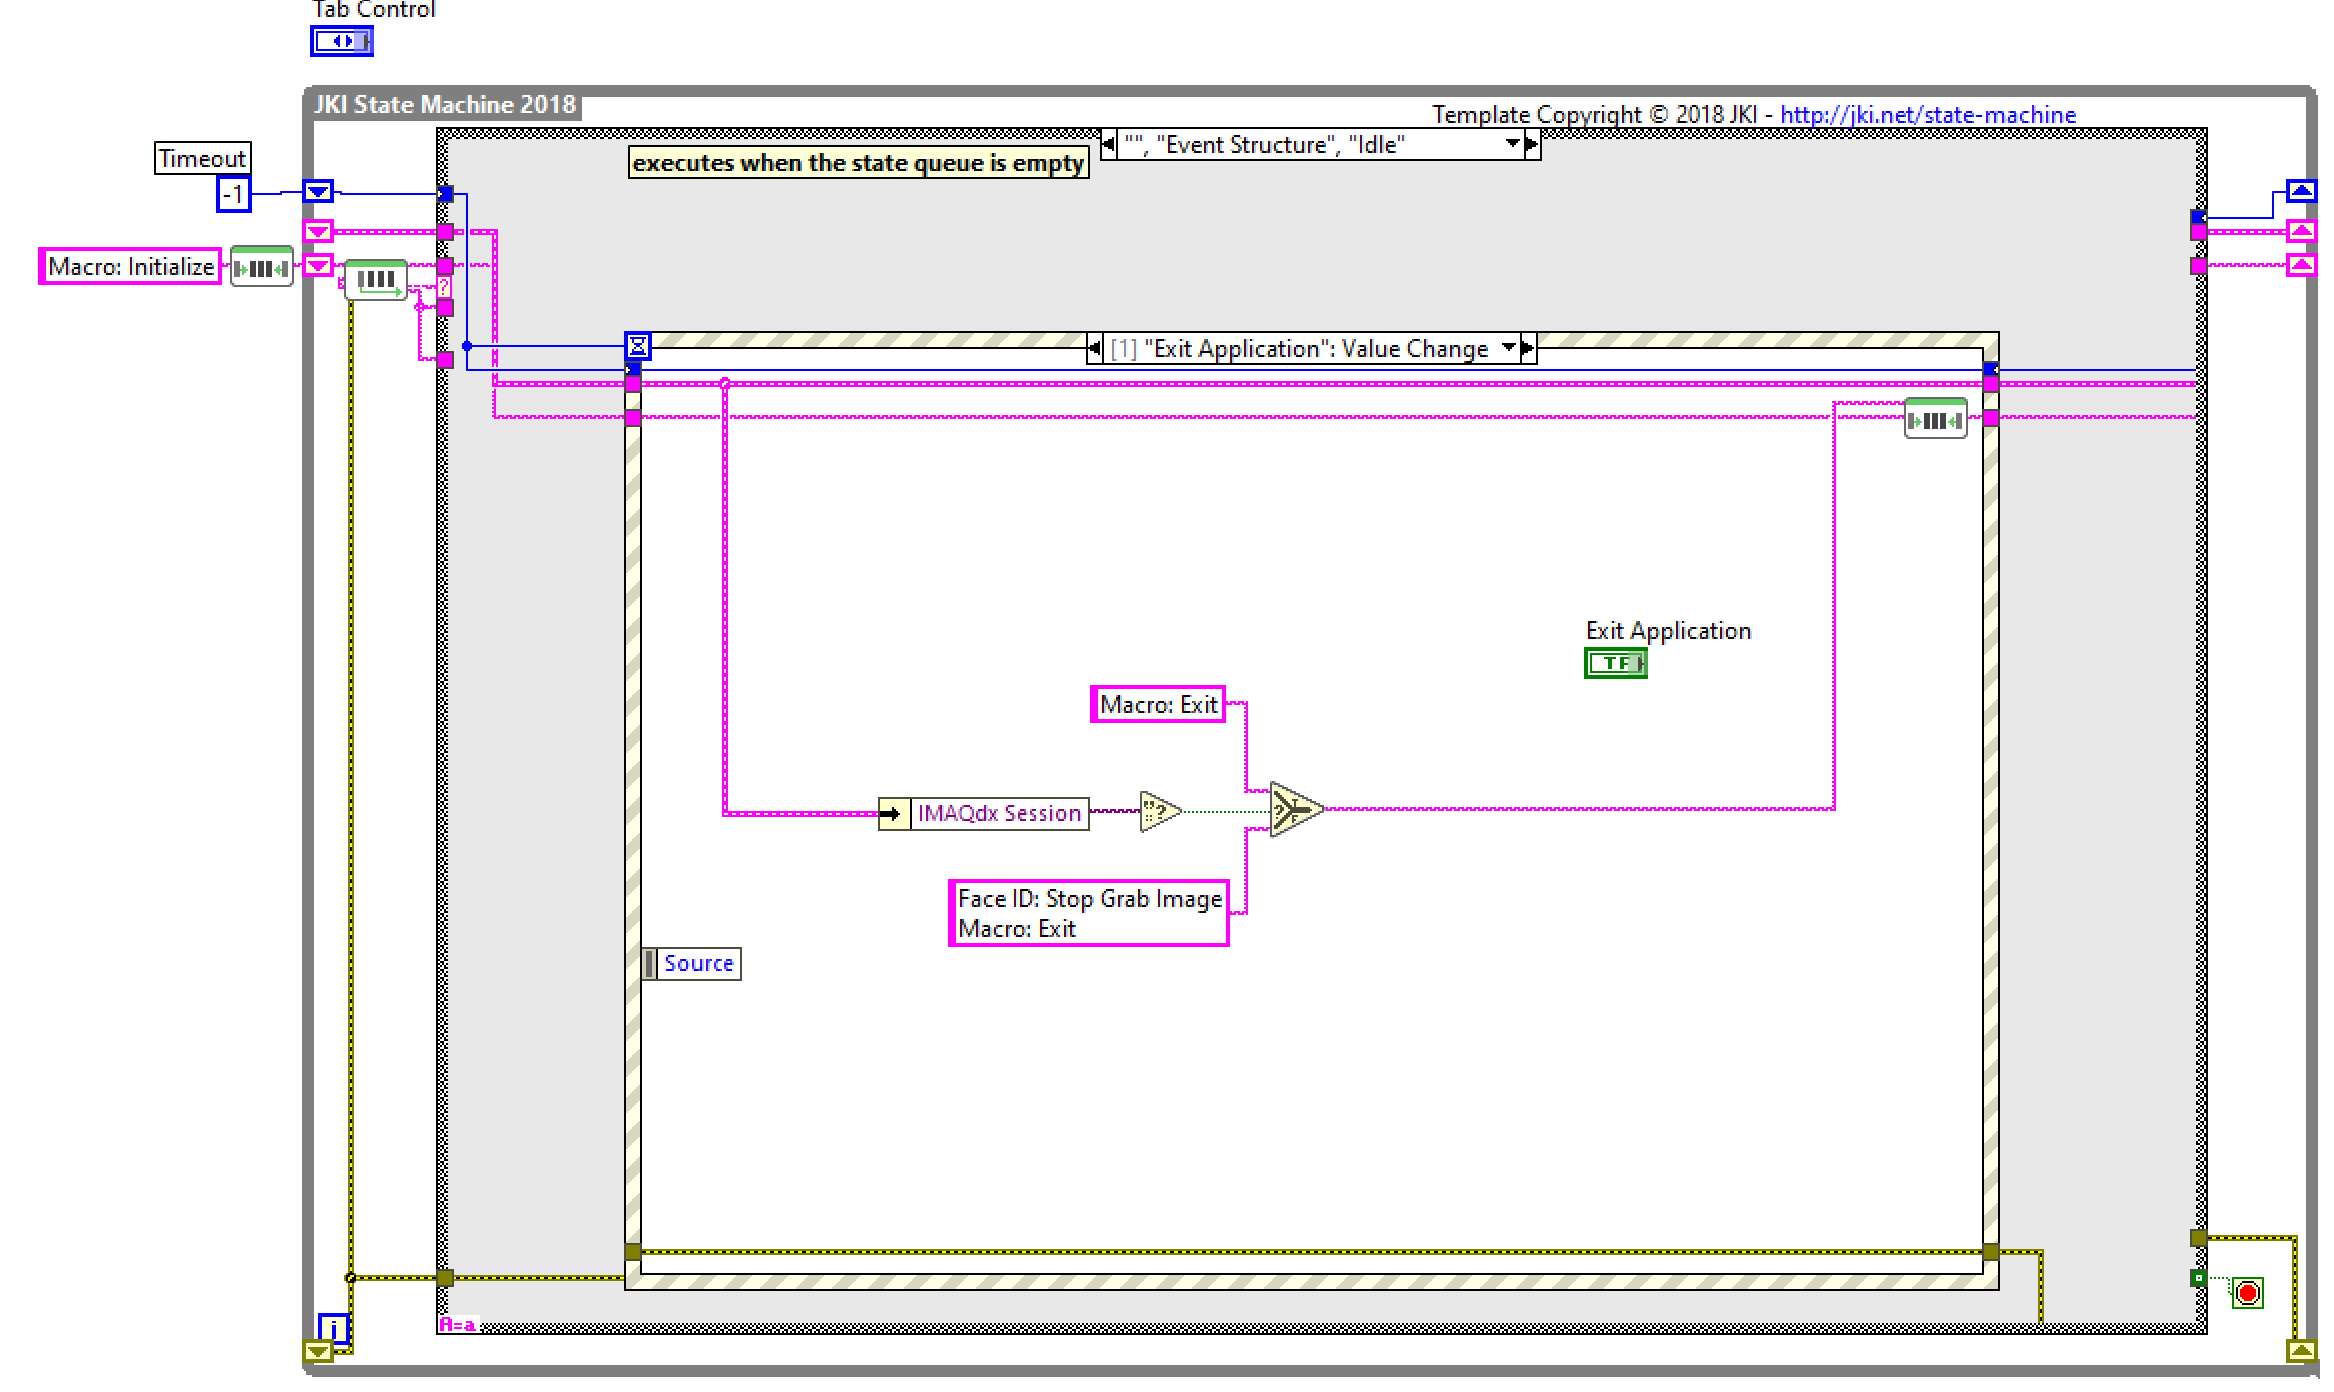
\includegraphics[width=1.0\textwidth]{"src/jki-main.png"}
    \caption{Zdjęcie przedstawiające podstawowy widok schemtu blokowego maszyny stanów JKI}
    \label{fig:foto1}
\end{figure}

Maszyna stanów JKI składa się z dwóch głównych elementów:
\begin{itemize}
    \item Pętli While,
    \item Struktury Case.
\end{itemize}

Pętla while odpowiada za nieskończone (naturalnie do momentu zdarzenia kończącego działania aplikacji) wykonywanie się aplikacji w pętli.
Podczas uruchomienia aplikacja rozpoczyna pracę w pętli oraz przechodzi przez kolejne stany (case) aplikacji.

Drugim elementem jest struktura Case, która odpowiada za naturę działania maszyny stanów - przechodzenie do odpowiednich stanów zdefiniowanych podczas uruchomienia oraz następnie zaciąganych z kolejki. 

\begin{figure} [H]
    \centering
    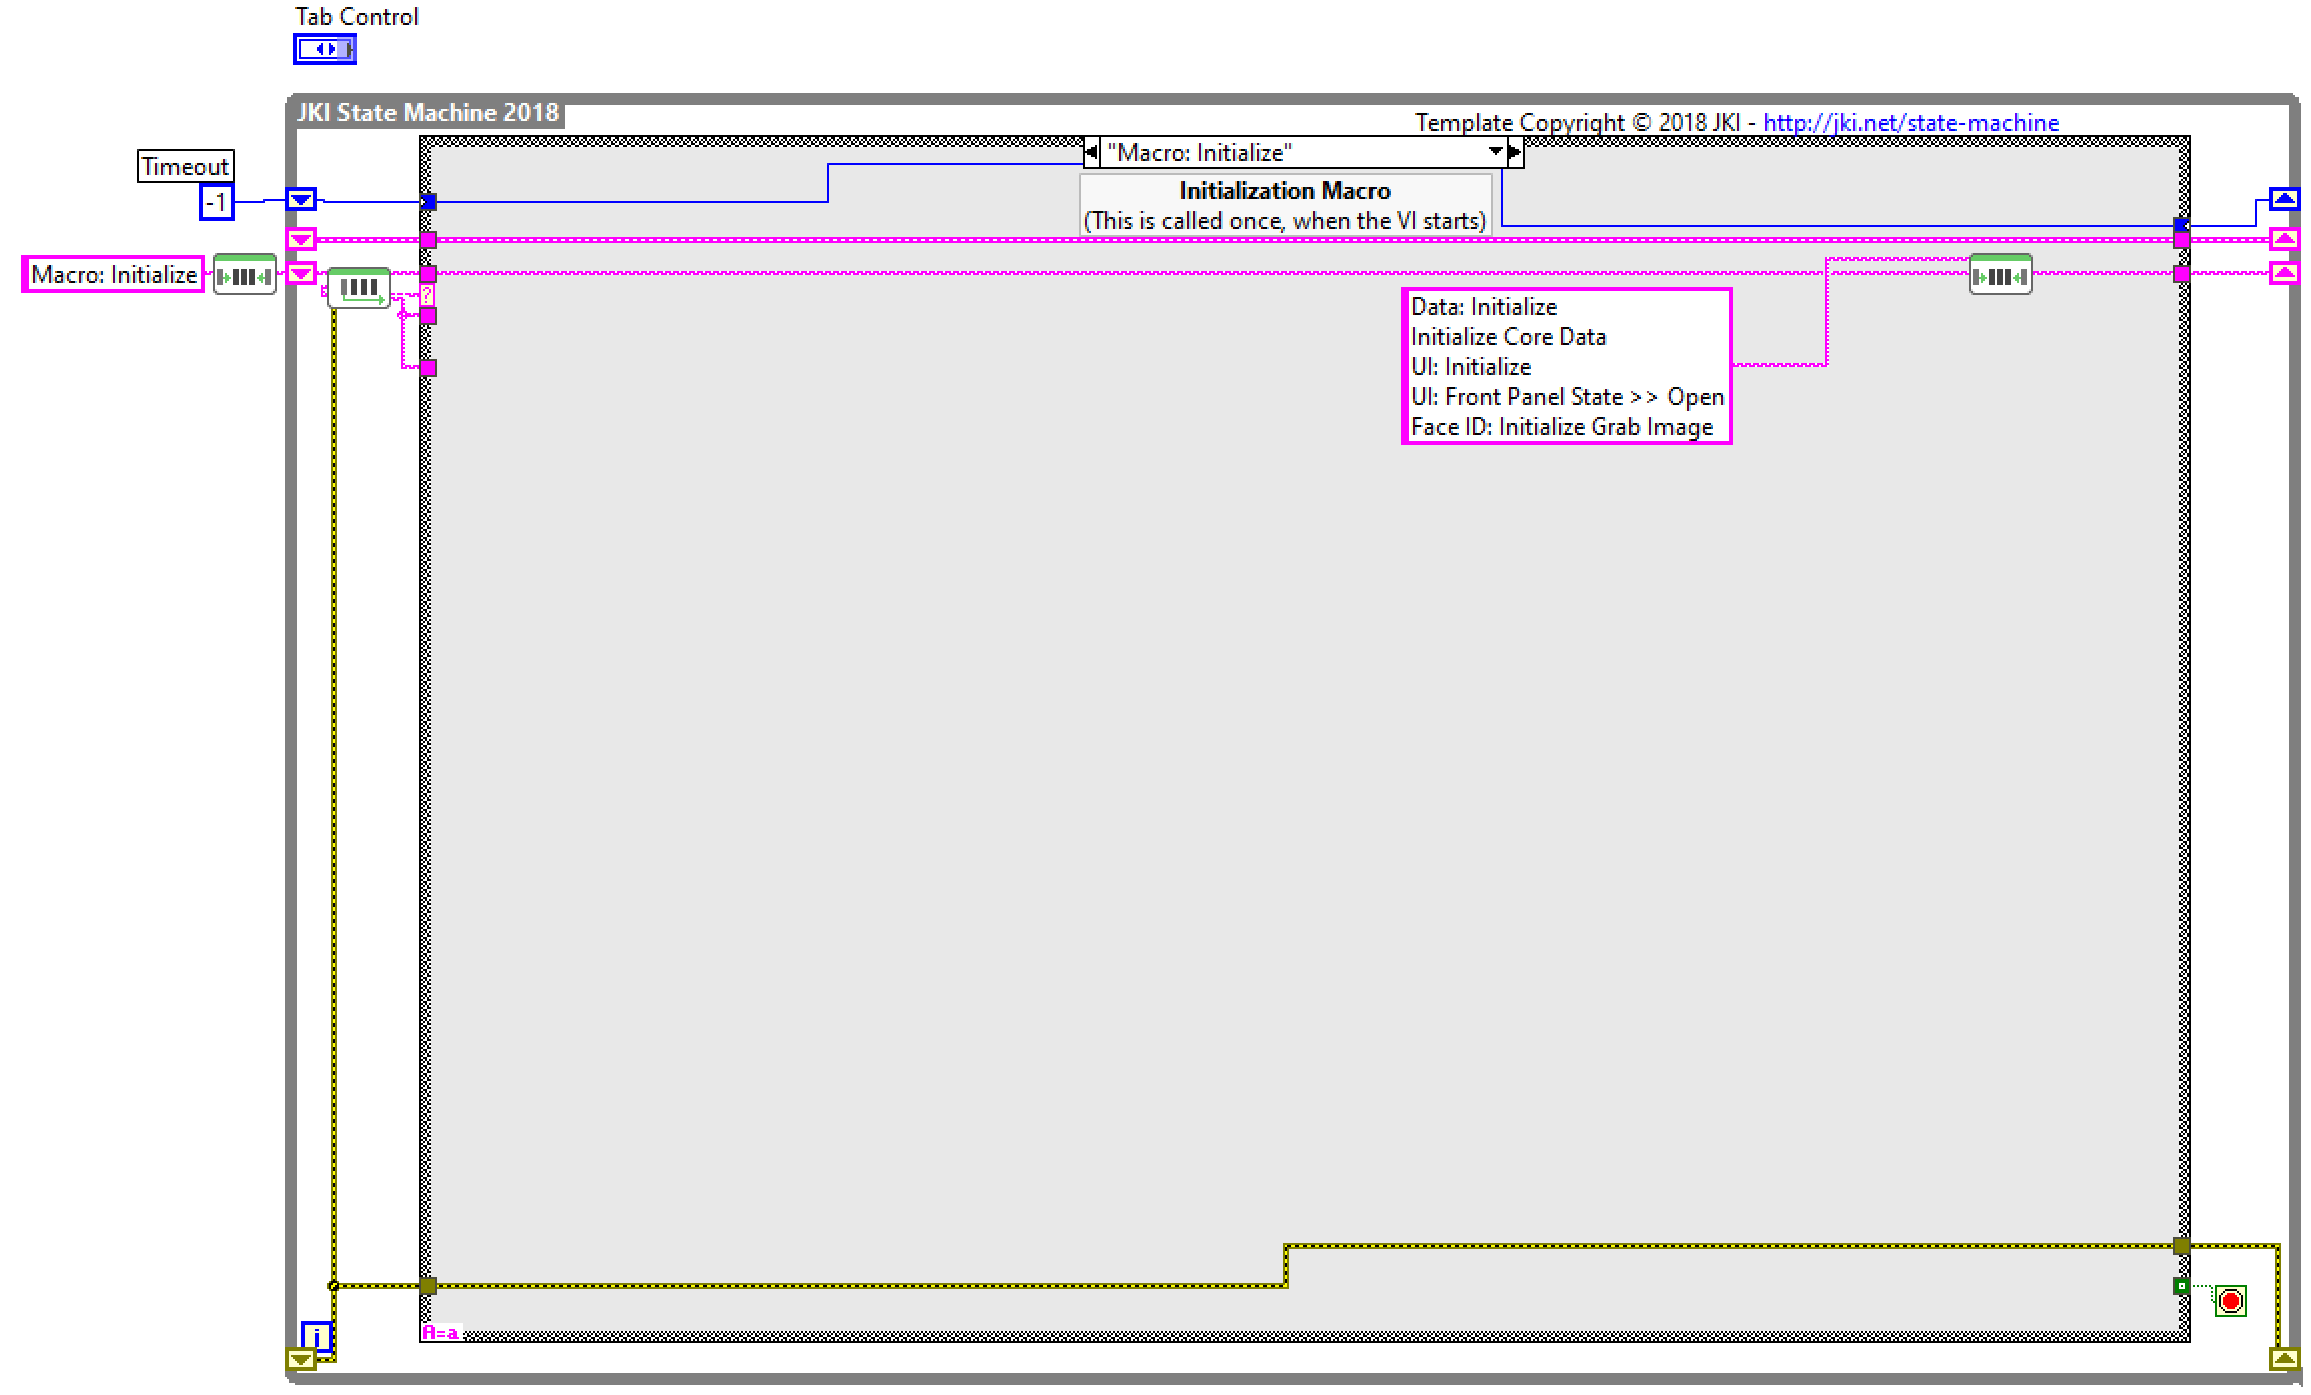
\includegraphics[width=1.0\textwidth]{"src/macro-init.png"}
    \caption{Zdjęcie przedstawiające stan "Macro: Initialize"}
    \label{fig:foto2}
\end{figure}

Stan "Macro: Initialize" jest wykonywany podczas startu aplikacji (jest to wyszczególnione pod rozwijaną listą ze stanami). Ważnym elementem jest pole statyczne typu String (oznaczone typowo kolorem różowym) 
zawierające pięć kolejnych stanów, które zostaną wysłane na kolejkę w celu odpowiedniego toku wykonywania. Najpierw wykona się stan Data: Initialize, następnie Initialize: Core Data etc. 
Na samym końcu zostanie wywołany stan Face ID: Initialize Grab Image. Jest to pierwszy stan, który nie jest zapewniony przez framework, a zatem kod napisany samodzielnie rozpoczyna się wraz z wywołaniem stanu piątego. 

\begin{figure} [H]
    \centering
    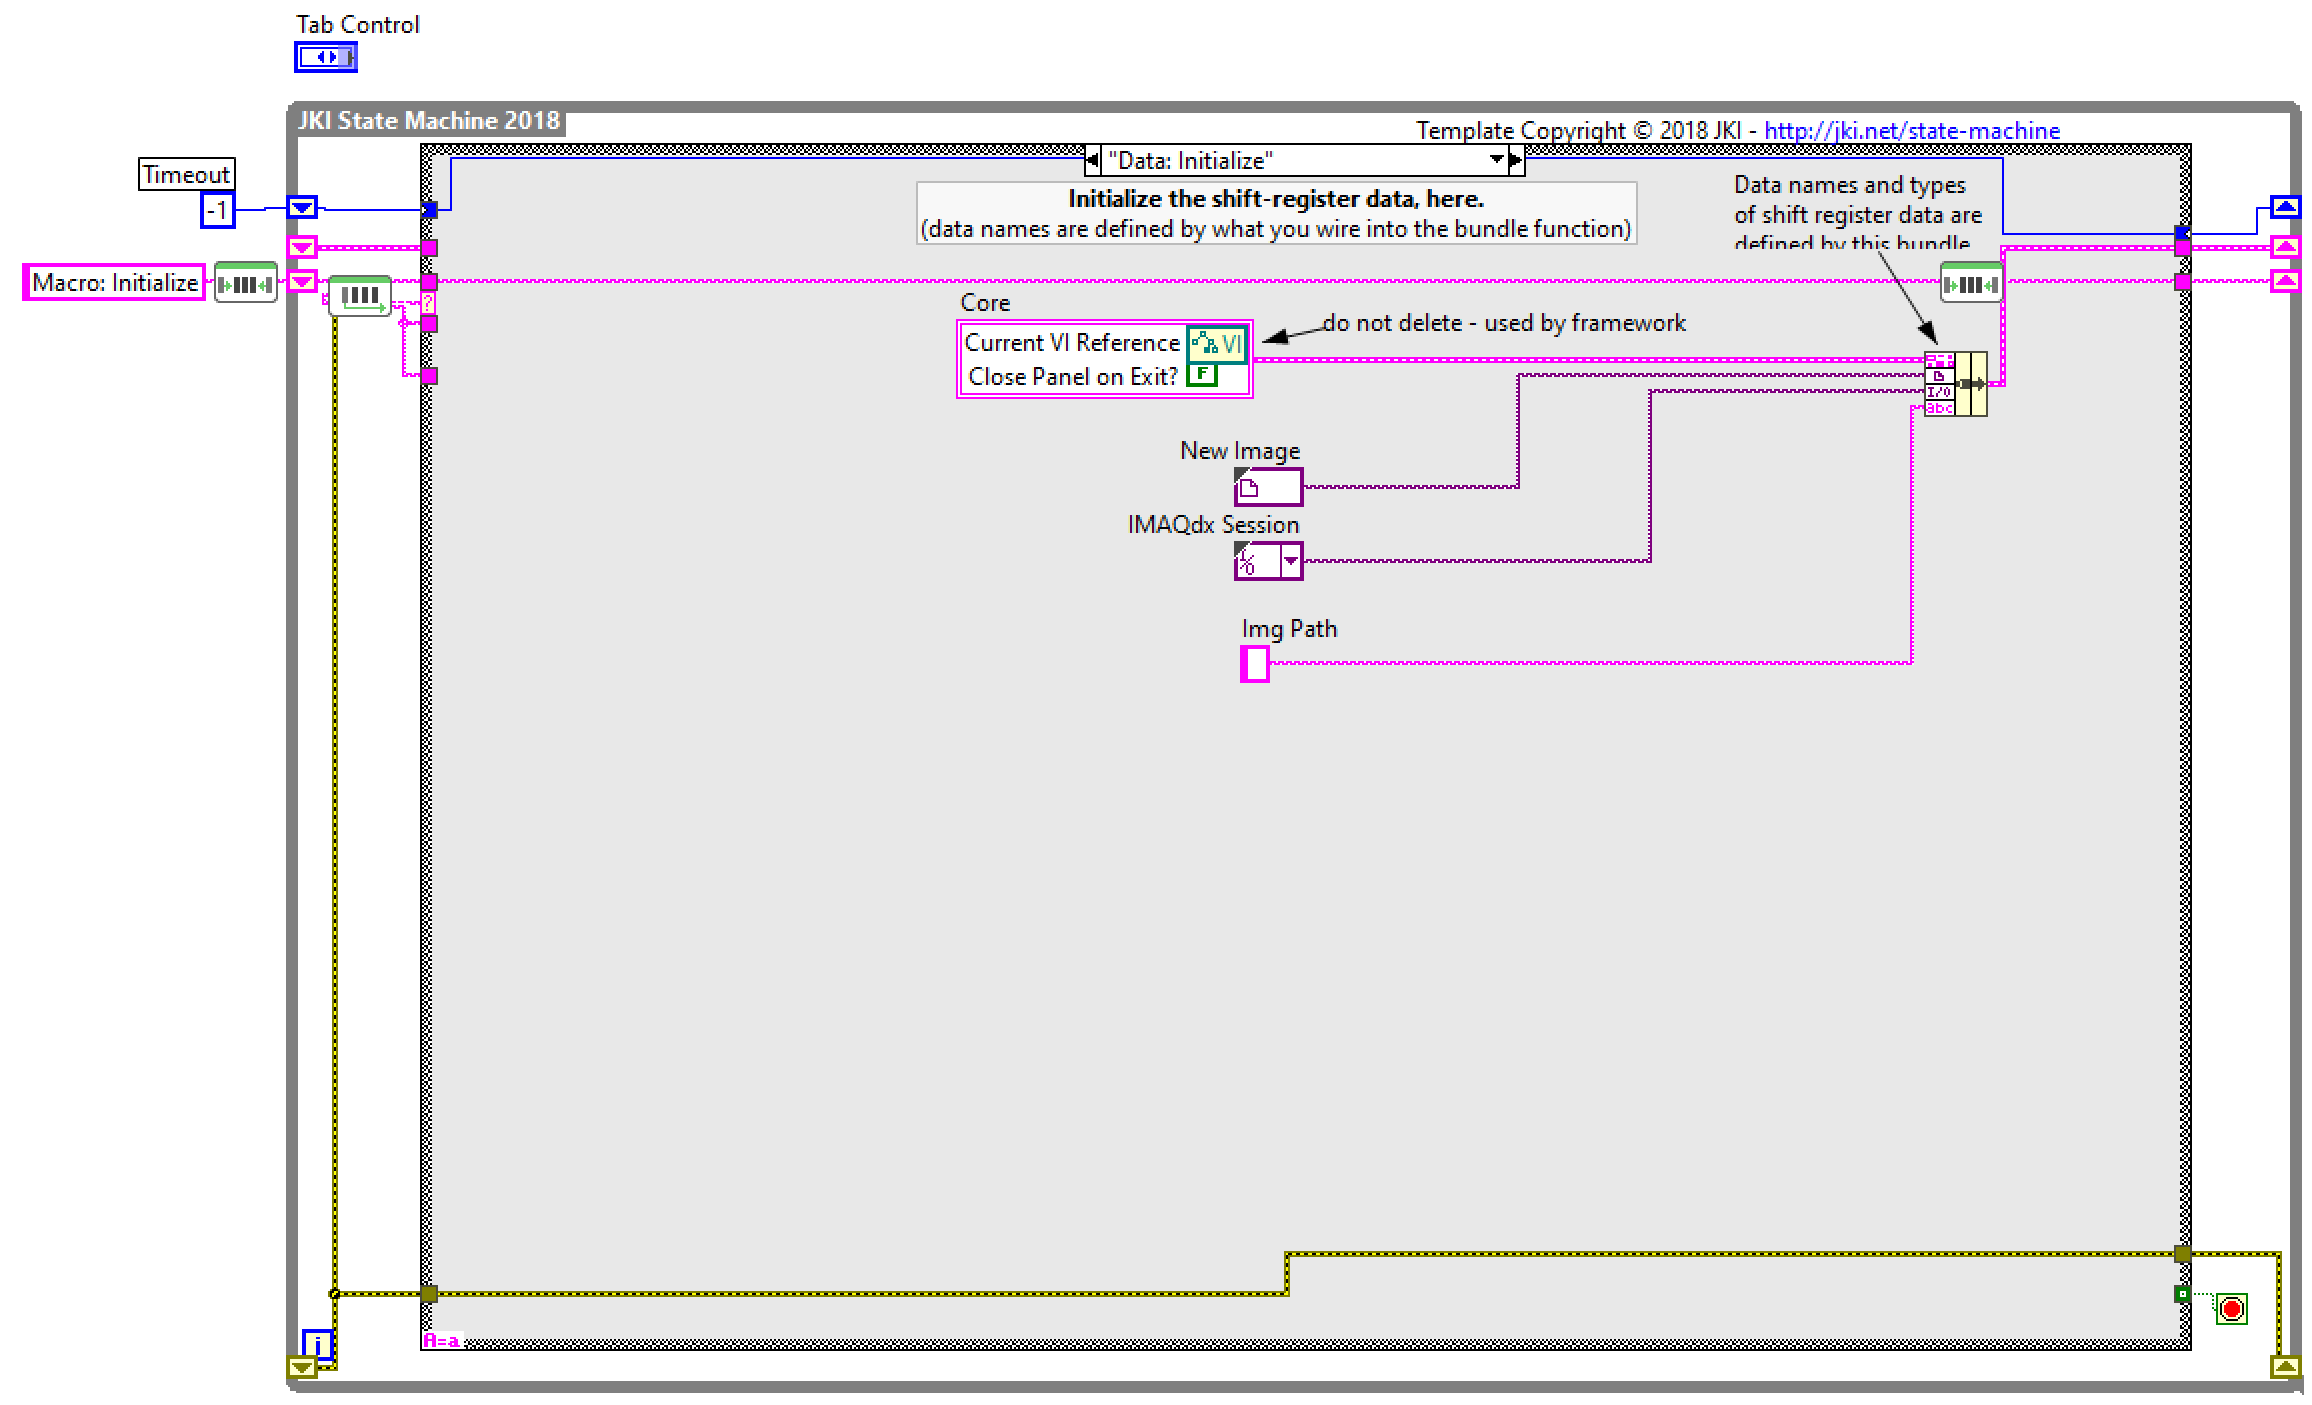
\includegraphics[width=1.0\textwidth]{"src/data-init.png"}
    \caption{Zdjęcie przedstawiające stan "Data: Initialize"}
    \label{fig:foto3}
\end{figure}

Stan "Data: Initialize" odpowiada za inicjalizację żyły zawierającej dane przepływające między stanami. Dzięki wykorzystaniu tej możliwości można przekazywać dowolne dane między kolejnymi stanami oraz modyfikować te dane. 
Dokładne wykorzystanie tej opcji zostanie zaprezentowane w dalszej części dokumentacji. 
Na potrzeby projektu linia danych jest inicjalizowana za pomocą trzech zmiennych:

\begin{itemize}
    \item New Image - przechowuje obraz, jest to zmienna typowa dla biblioteki IMAQ,
    \item IMAQdx Session - kolejna zmienna typowa dla biblioteki IMAQ, przechowuje referencję do otwartek sesji kamery,
    \item Img Path - zmienna typu String przechowująca ściezkę do nowo pobranego zdjęcia.
\end{itemize}

\begin{figure} [H]
    \centering
    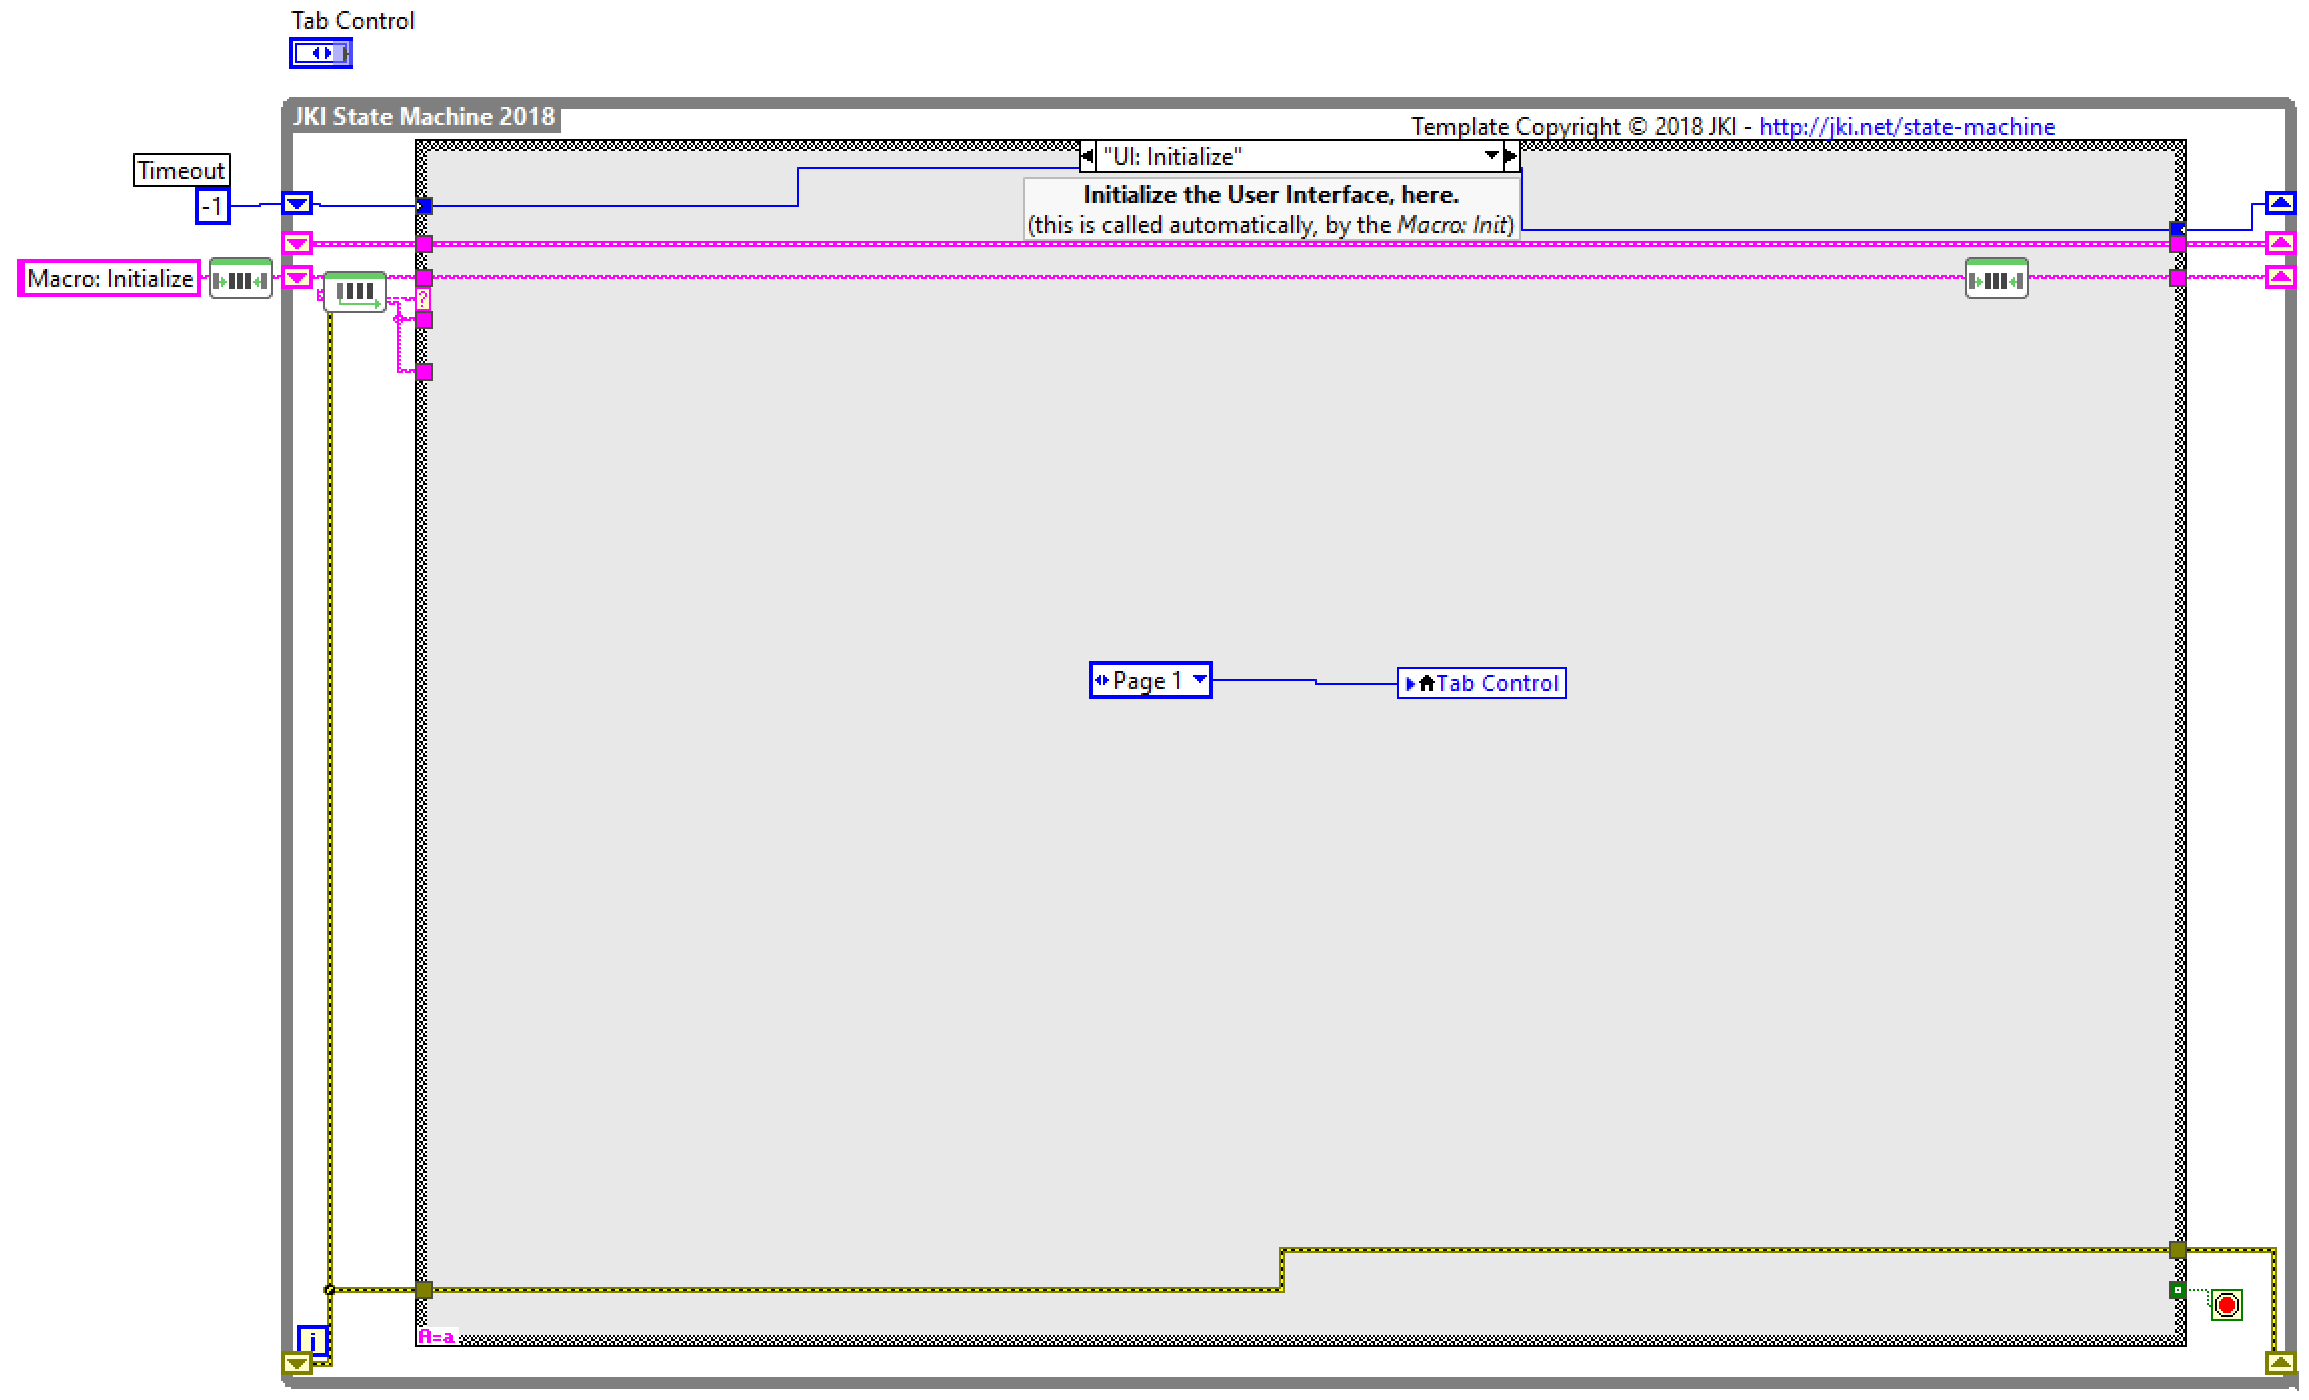
\includegraphics[width=1.0\textwidth]{"src/UI-init.png"}
    \caption{Zdjęcie przedstawiające stan "UI: Initialize"}
    \label{fig:foto4}
\end{figure}

Stan "UI: Initialize" odpowida za wyświetlenie podstawowego widoku aplikacji. W przypadku powyższego projektu odpowiada on za wyświetlenie 
pierwszej zakładki aplikacji przy pomocy struktury Tab dostarczanej przez LabVIEW. 
Element "Page 1" jest standardowym typem wyliczeniowym enum zawierającym deklaracje poszczególnych zakładek. 
Element "Tab Control" odpowiada za wyświetlenie odpowiedniej strony na podstawie wybranej opcji w typie wyliczeniowym.


\subsection{\Large Implementacja procesu logowania w LabView}
Proces logowania jest procesem złożonym z kilku stanów, każdy stan zostanie szczegółowo opisany w poniższej sekcji. 

\subsubsection{\large Stan Face ID: Initialize Grab Image}
Stan "Face ID: Initialize Grab Image" obejmuje procedurę inicjalizacji kamery, niezbędną do późniejszego akwizycji obrazu. W strukturze blokowej tego stanu, centralną rolę pełni struktura "Case", która odpowiada za odpowiednią reakcję aplikacji na wybór kamery. Blok "List Cams" jest opcjonalny, lecz zaleca się jego użycie w przypadku dostępności wielu kamer, umożliwiając użytkownikowi wybór preferowanej. Po dokonaniu wyboru kamery, program przechodzi do kolejnego bloku, który sprawdza dostępność oraz poprawność działania kamery. Z tego bloku wynika binarna flaga, wyznaczająca stan struktury "Case" zgodnie z wynikiem wyboru kamery. Warto zaznaczyć, że blok "Select Camera" zwraca wartość True, jeśli kamera nie została znaleziona lub nie udało się jej poprawnie zainicjalizować; w przypadku powodzenia zwraca False.

W przypadku uzyskania wartości False, odpowiedni stan struktury case zostaje wykonany. Na wejście struktury przekazywane są aktualne stany w kolejce oraz linia Timeout. W centralnej części znajdują się bloki finalizujące konfigurację kamery oraz jej przygotowanie do użycia. Dodatkowo, do linii danych przekazywana jest sesja kamery utworzona przez blok "Configure Grab", oraz pusta referencja do nowego obrazu, który zostanie nadpisany w kolejnym kroku. Ponadto, stan "Face ID: Grab Image" jest dodawany do kolejki jako następny do wykonania.

\begin{figure}[H]
    \centering
    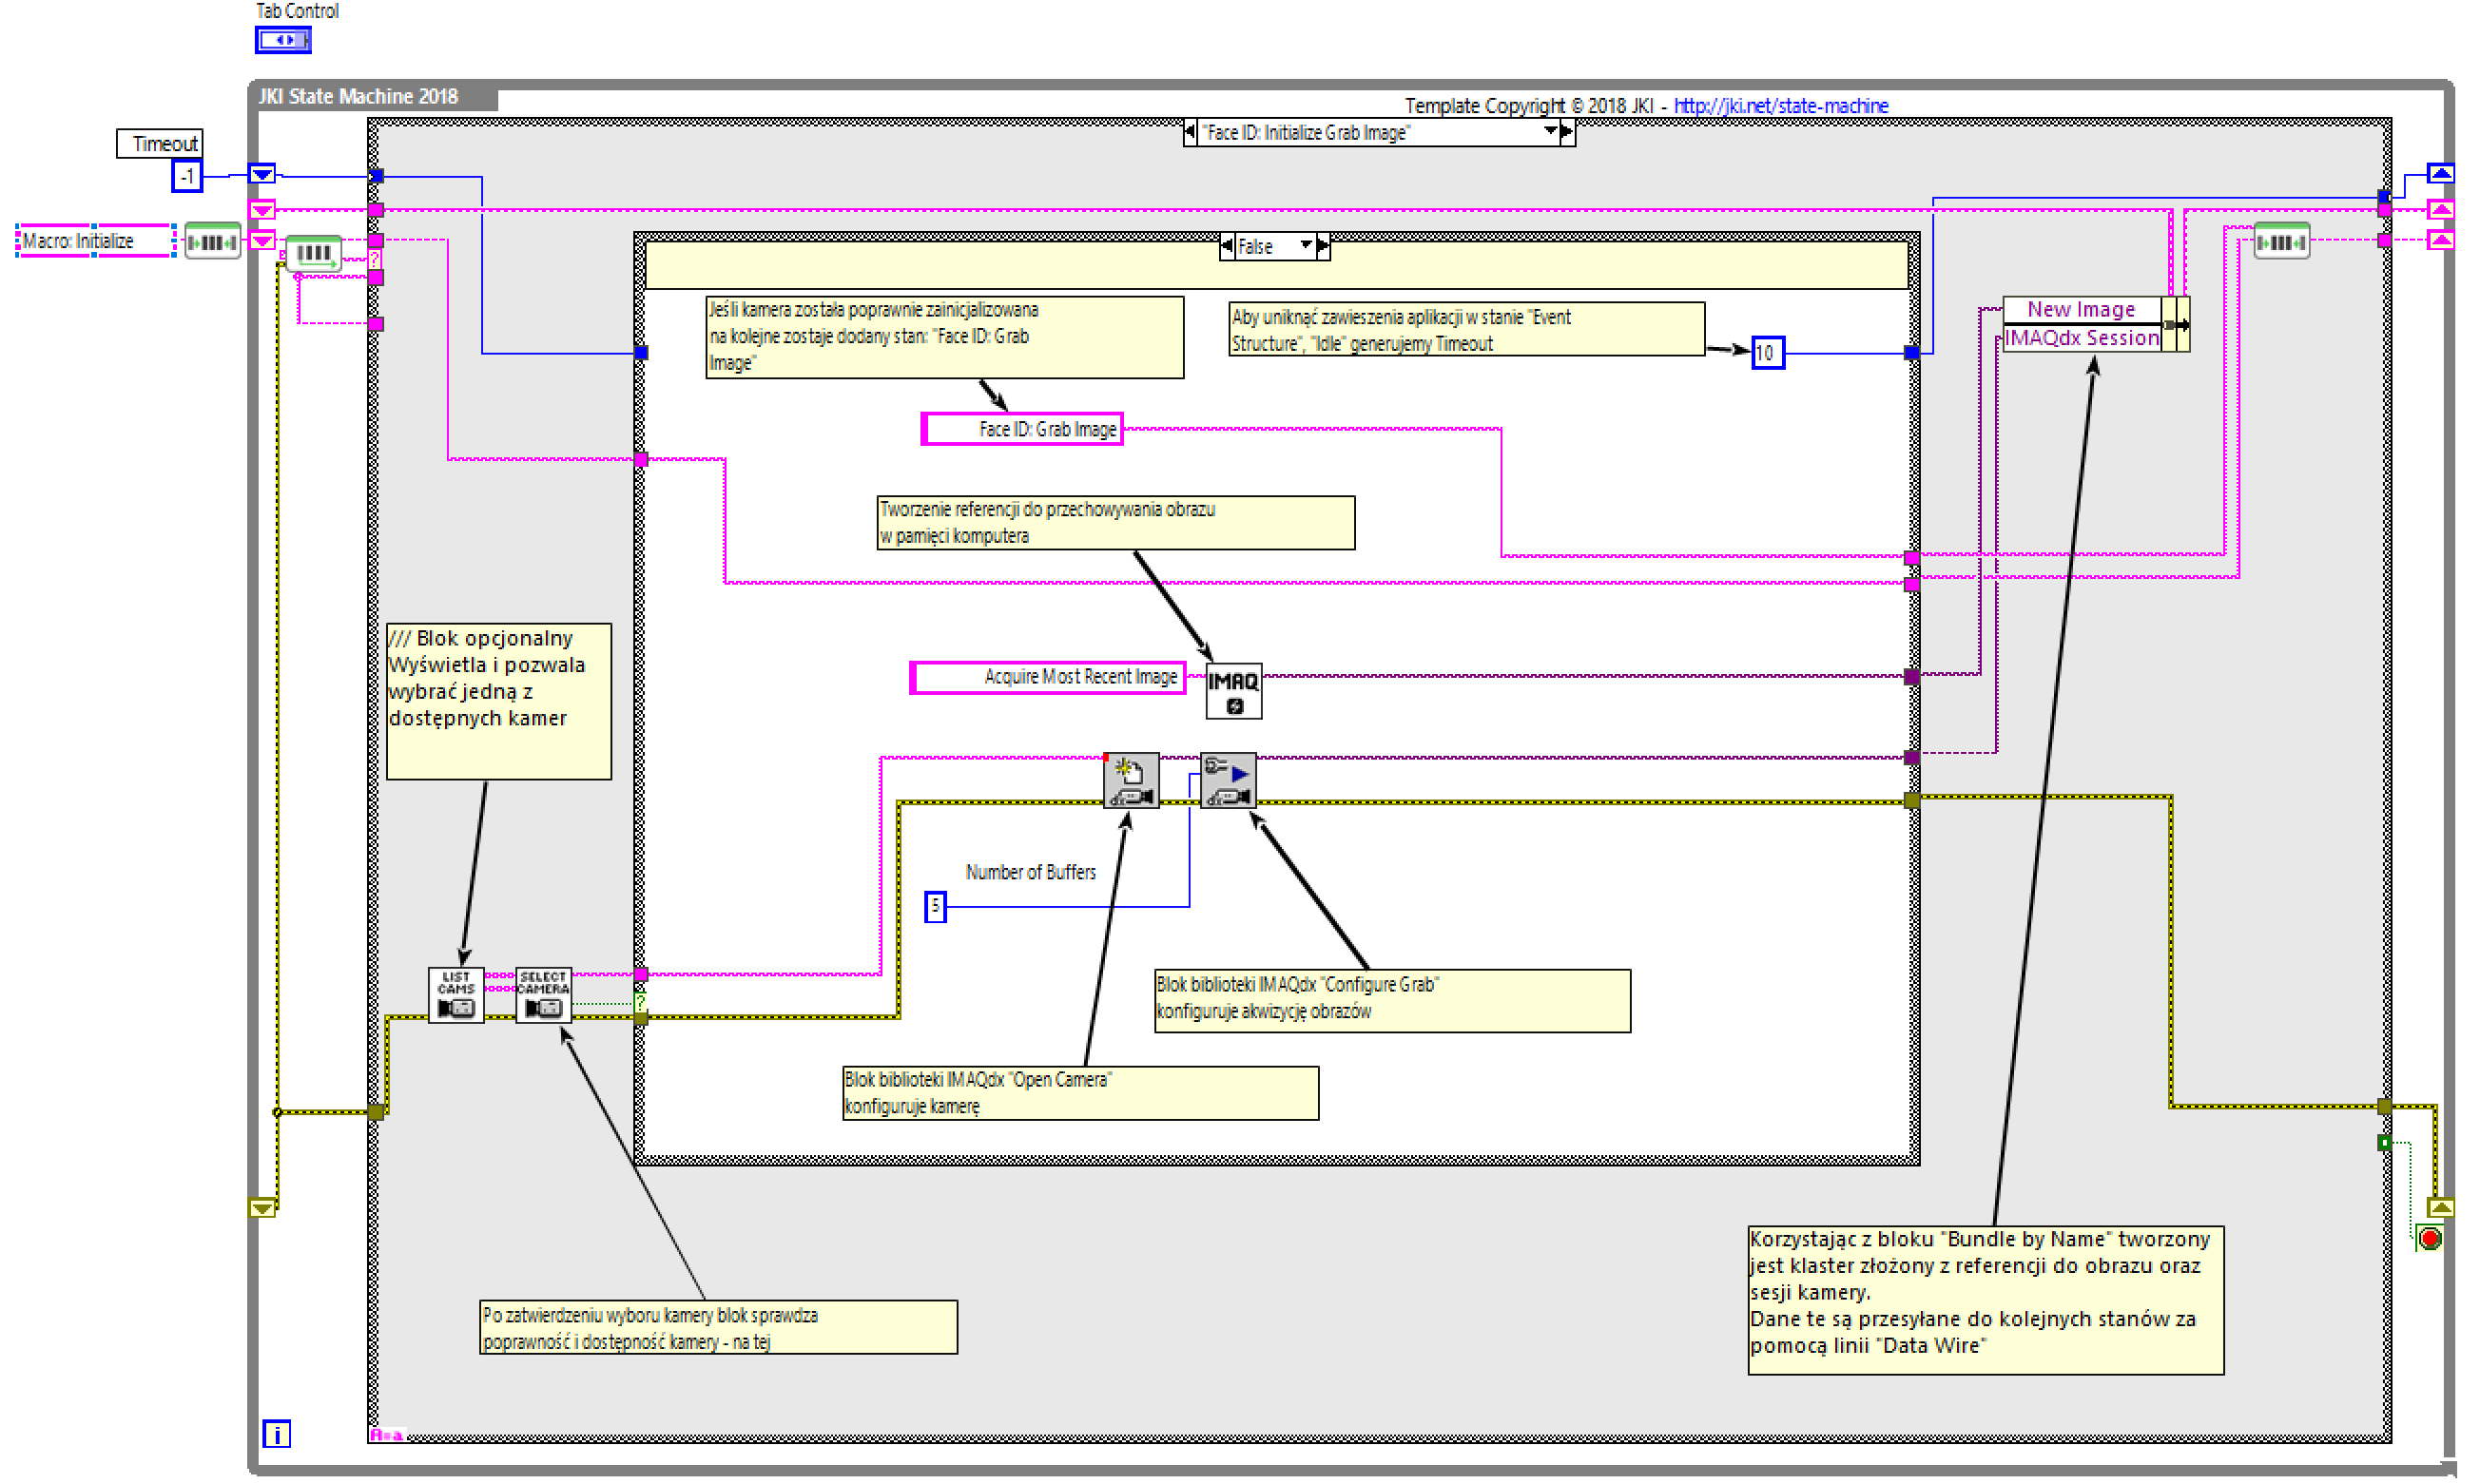
\includegraphics[width=1.0\textwidth]{src/face-id/face-id-init.png}
    \caption{Zdjęcie przedstawiające stan "Face ID: Initialize Grab Image" jeśli kamera została znaleziona poprawnie}
    \label{fig:face_id-init_false}
\end{figure}

Należy zwrócić uwagę na nadpisanie domyślnego Timeout, mające na celu zabezpieczenie aplikacji przed zatrzymaniem w stanie "Idle", czyli bezczynnością.

Jeśli zostanie uzyskana wartość True, a zatem kamera nie została znaleziona, na kolejkę zostaje wysłany stan "Error Handler" oraz wszystkie inne stany zostają usunięte. 
Dodatkowo do linii danych zostaje przesłana pusta referencja do sesji kamery oraz pusta referencja do obrazu. 

Warto zauważyć, że w tym przypadku timeout pozostaje niezmieniony względem jego dymyślnej wartości. 

\begin{figure}[H]
    \centering
    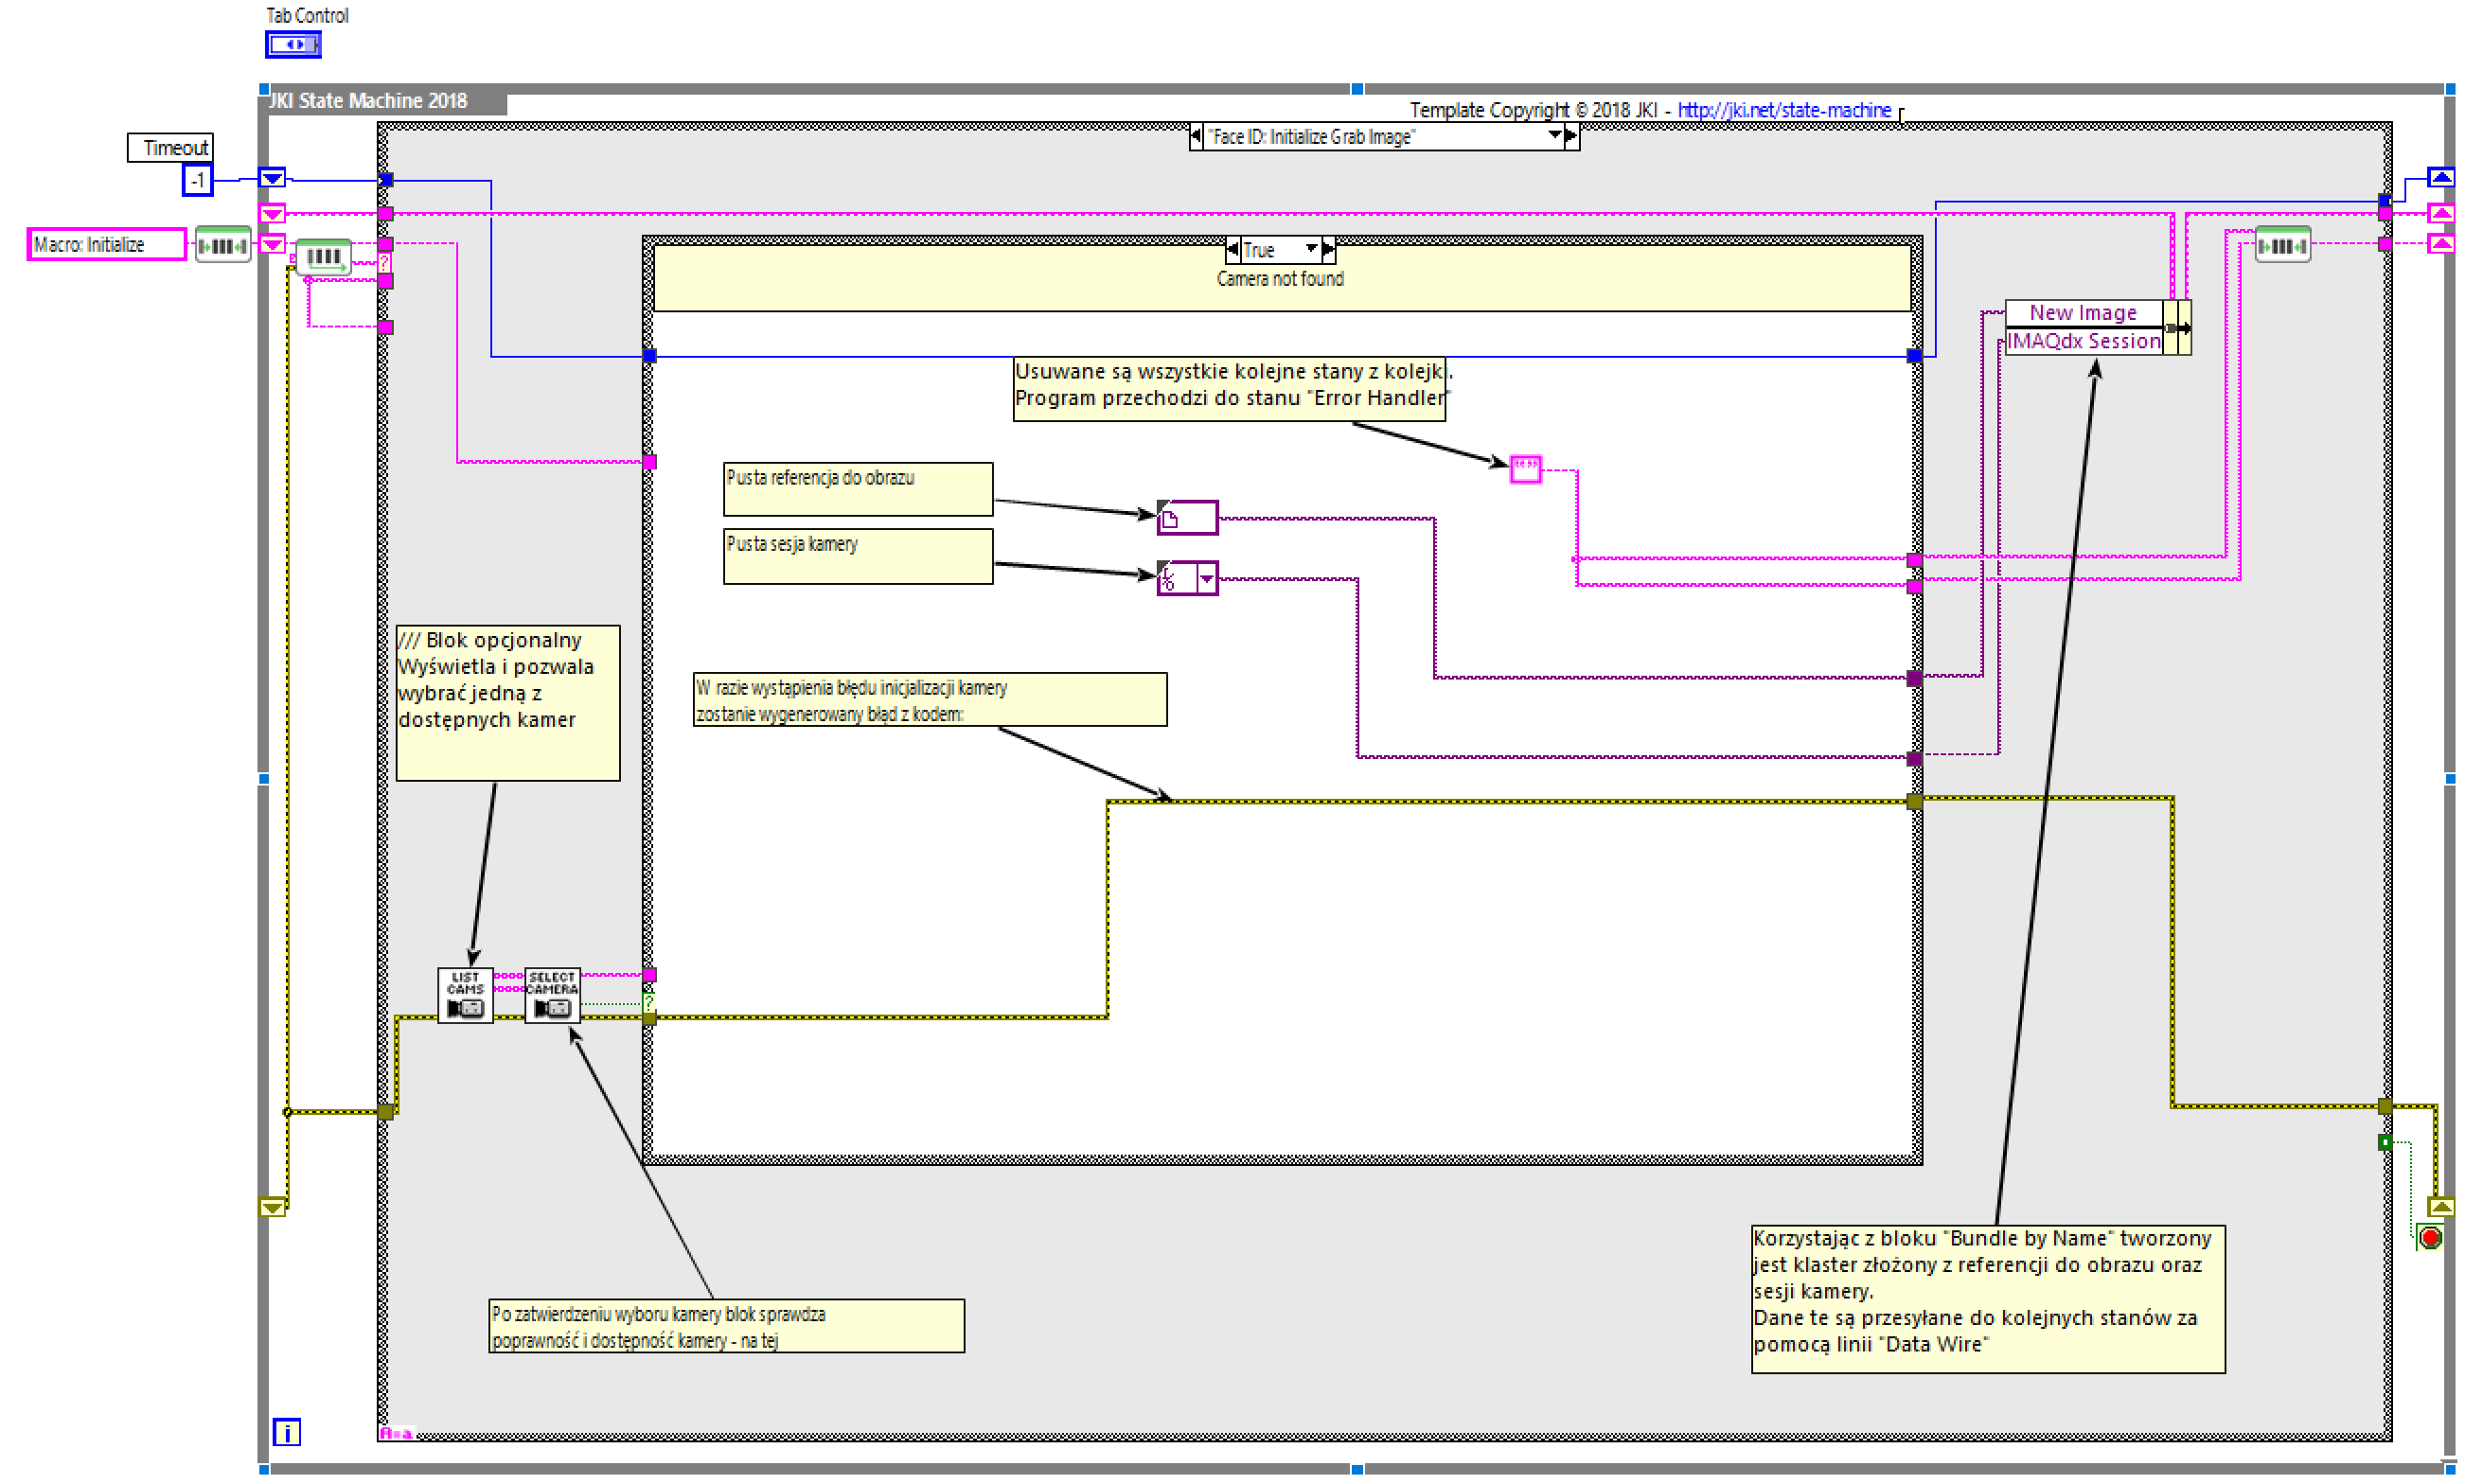
\includegraphics[width=1.0\textwidth]{src/face-id/face-id-init-T.png}
    \caption{Zdjęcie przedstawiające stan "Face ID: Initialize Grab Image" jeśli kamera nie została znaleziona poprawnie}
    \label{fig:face_id-init_true}
\end{figure}

\subsubsection{\large Stan Face ID: Grab Image}

Stan "Face ID: Grab Image" odpowiada za właściwą akwizycję obrazu oraz jego wyświetlenie na interfejsie użytkownika. 

Pierwszym elementem widoczym na schemacie blokowym jest blok "Unbundle by Name", który odpowiada za wyodrędnienie danych przesyłanych poprzez linię danych jako klaster. Drugim elementem jest przycisk, mający na celu rozpoczęcie akwizycji obrazu. W centralnym punkcie schematu znajduje się blok "Take Image Case Struct". Jest to plik SubVi, który przechowuje logikę pobierania obrazu. Na wejścia tego bloku należy poprowadzić:
\begin{itemize}
    \item IMAQdx Session - aktualną sesję kamery,
    \item New Image - Referencję do obrazu,
    \item Przycisk odpowiedzialny za rozpoczęcie procesu logowania,
    \item Error In - Błąd.
\end{itemize}

Na wyjściach bloku znajdują się:
\begin{itemize}
    \item IMAQdx Session - Aktualną sesję kamery,
    \item New Image - Referencję do pobranego obrazu,
    \item Kolejne stany do kolejki,
    \item Error Out - Błąd wyjściowy.
\end{itemize}

Kolejnym istotnym elementem jest blok Image Display, odpowiada on za wyświetlenie pobranego obrazu na interfejsie użytkownika.

Ostatnim elementem znajdującym się na schemacie jest blok "Bundle By Name", którego działanie jest odwrotne do działania bloku "Unbundle By Name", zatem tworzy on klaster danych poprzez połączenie kilku danych wejściowych.

\begin{figure}[H]
    \centering
    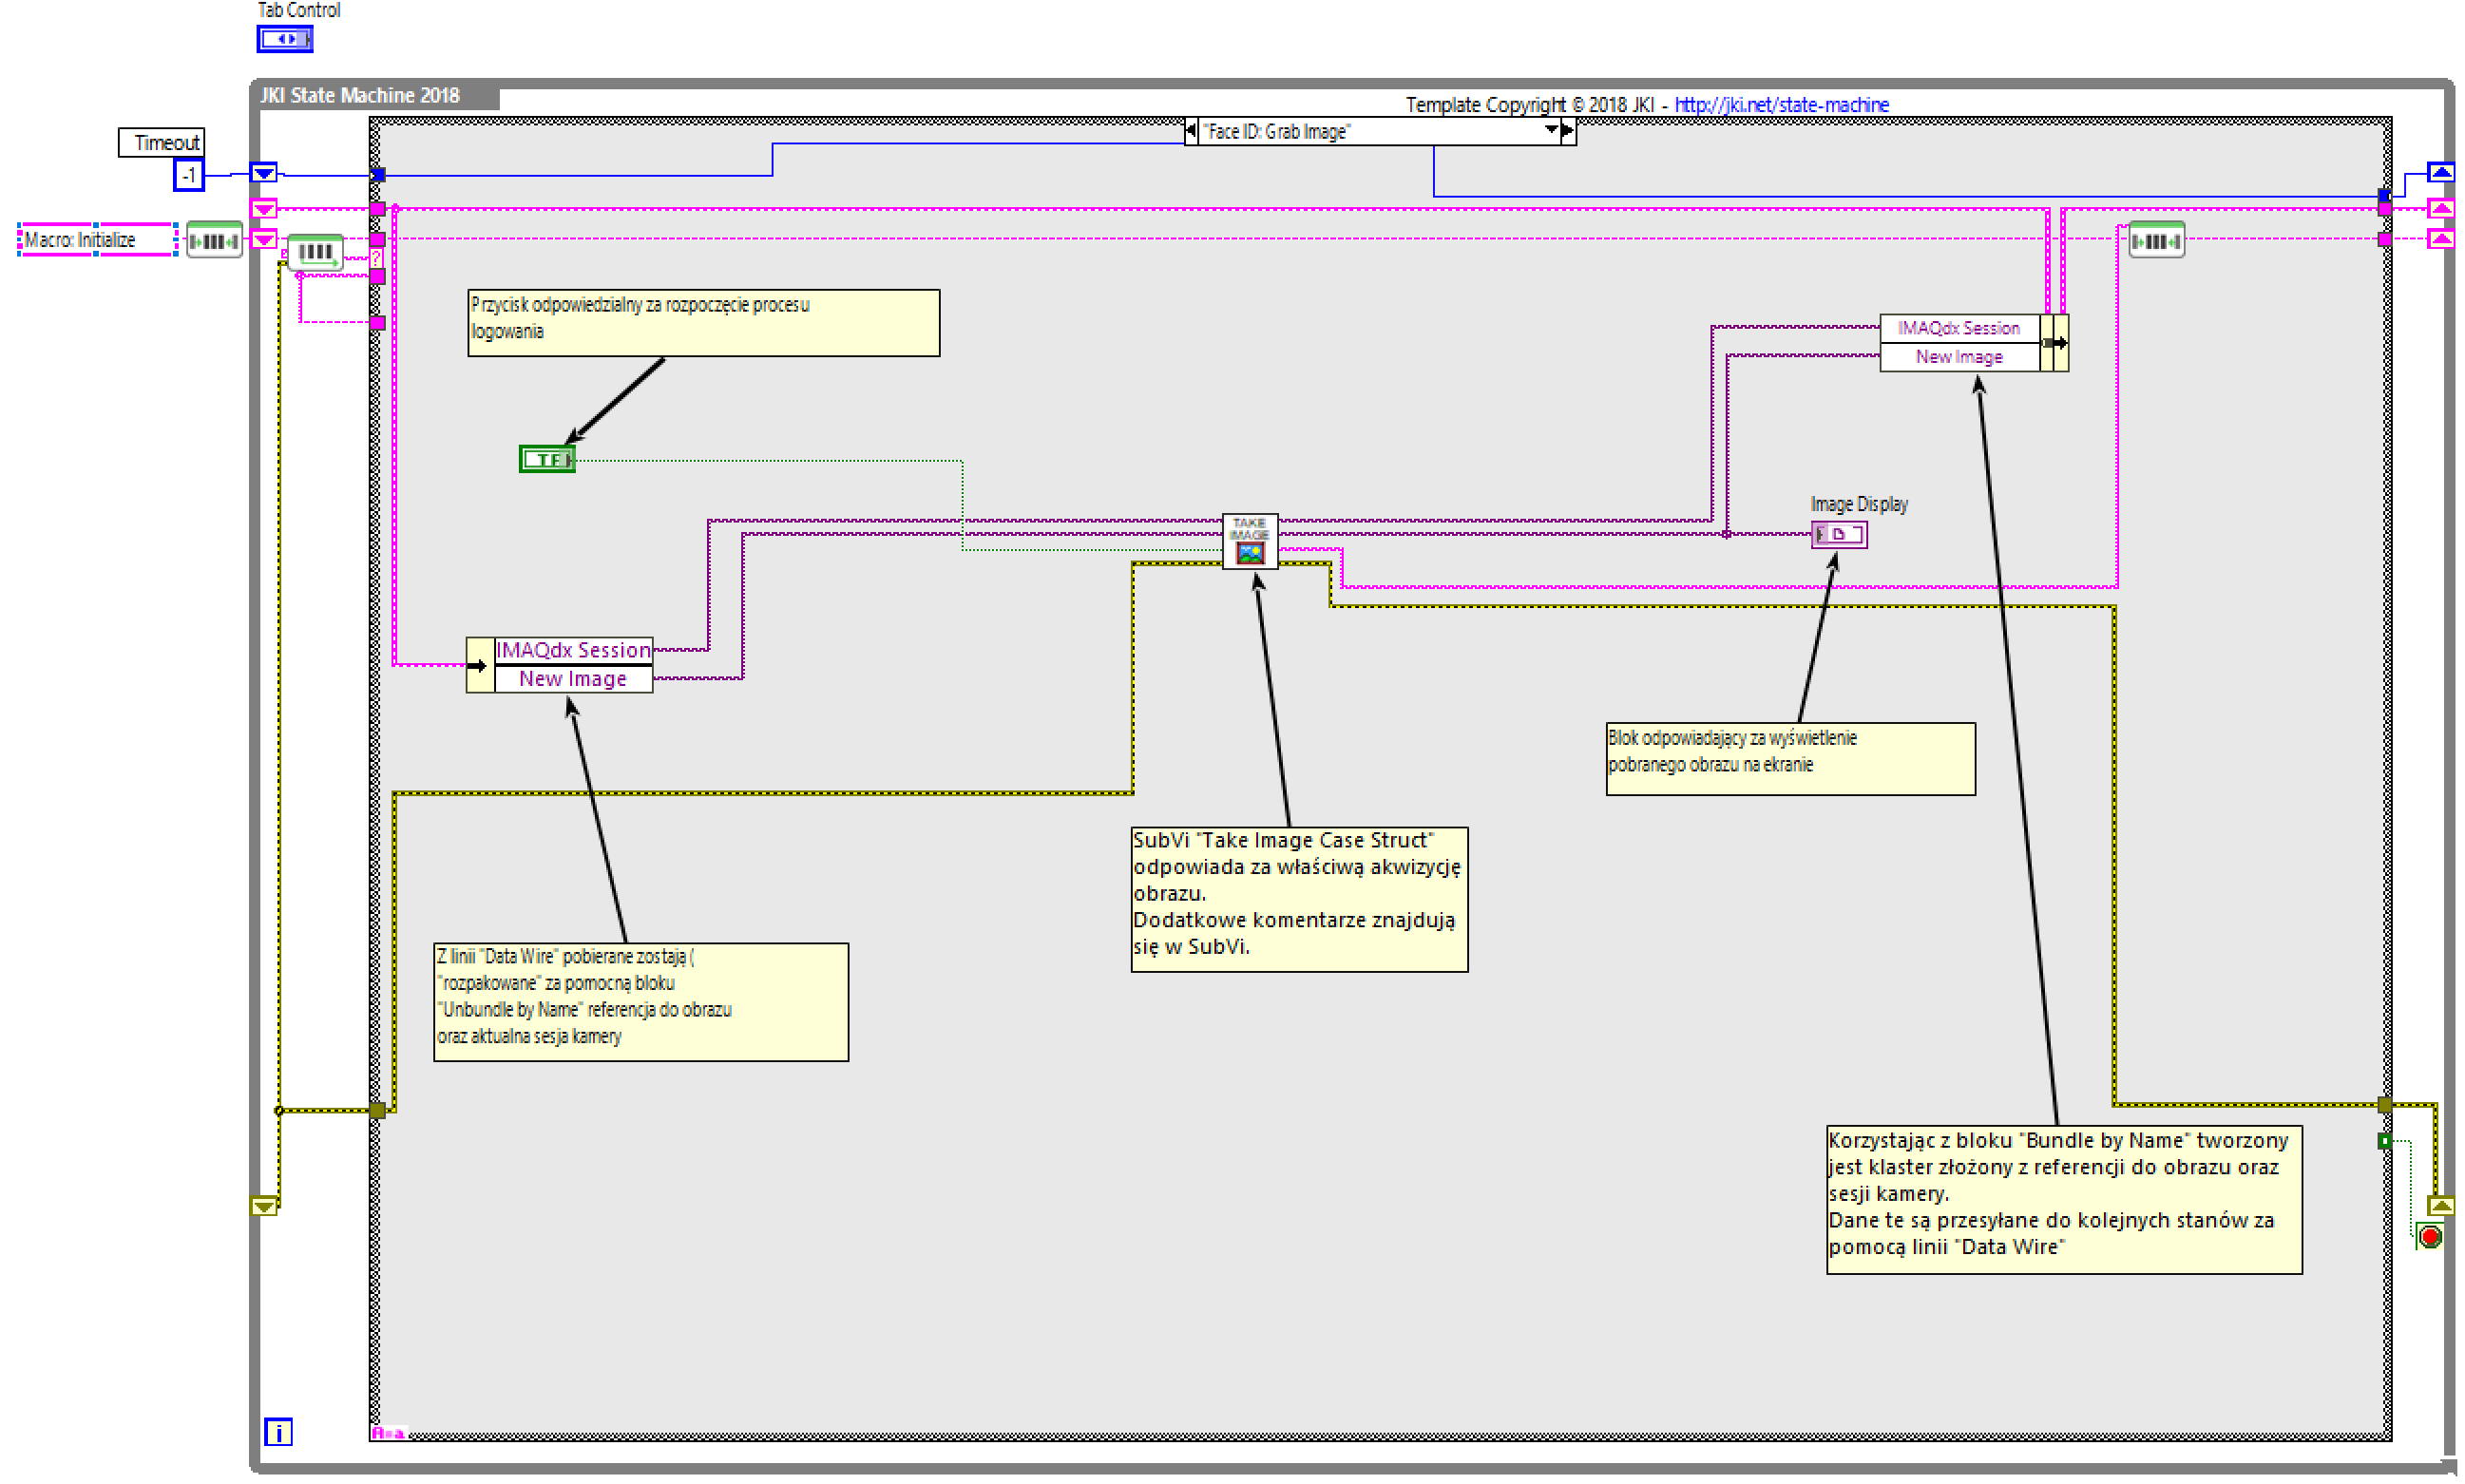
\includegraphics[width=1.0\textwidth]{src/face-id/face-id-grab.png}
    \caption{Zdjęcie przedstawiające stan "Face ID: Grab Image"}
    \label{fig:face_id-grab}
\end{figure}

\subsubsection*{Take Image Case Struct - SubVi}

Jak wspomniano wcześniej, powyższy SubVi odpowiada za logikę pobrania zdjęcia. Ze względu na dbałość o czyistość i przejrzystość kodu w przypadku dużej ilości bloków, należy starać się wyodrębnić część bloków do SubVi właśnie. Naturalnie wejścia oraz wyjścia są takie same jak opisane wyżej, dlatego nie będą ponownie wyszczególniane. 

Rdzeniem tego SubVi jest struktura Case, która na podstawie stanu przycisku odpowiednio wykonuje stan True lub False. 
Jeśli stan przycisku jest równy False, obraz jest pobierany przez blok "Get Image2", a następnie przekazywany na wyjście wraz z trwającą sesją kamery. Natomiast do kolejki zostaje przekazany stan "Face ID: Grab Image", co oznacza zapętlenie maszyny stanów w tym stanie dopóki nie nastąpi naciśnięcie przycisku "Exit" kończącego działanie całej aplikacji lub nie zostanie naciśnięty przycisk logowania. 

W przypadku naciśnięcia przycisku logowania, zostaje wykonany stan True. Proces pobierania obrazu oraz przekazywania jego referencji na wyjście jest niezmieniony. Różnica pojawia się natomiast w sposobie przekazywania kolejnego stanu do kolejki. Poczynając od środka, można zauważyć blok "Elapsed Time", jest on odpowiedzialny za licznik, który określa jak długo ma trwać akwizycja danych. Jeśli licznik jest w trakcie odliczania, na jego wyjściu pojawia się flaga "False" i trafia na blok "Select", który jest odpowiedzialny za wybór odpowiedniej wartości na podstawie warunku. Można porównać ten blok do prostej instrukcji warunkowej if. Zatem jeśli licznik jest w trakcie działania, do kolejki jest przekazywany stan "Face ID: Grab Image" oraz grupa stanów "Event Structure". To oznacza, że ponownie tak długo jak trwa timer, aplikacja będzie zapętlona na stanie "Face ID: Grab Image". W momencie, gdy licznik zwróci wartość True - odliczy zadany czas, do kolejki zostaje przekazany stan "Face ID: Stop Grab Image". 

\begin{figure}[H]
    \centering
    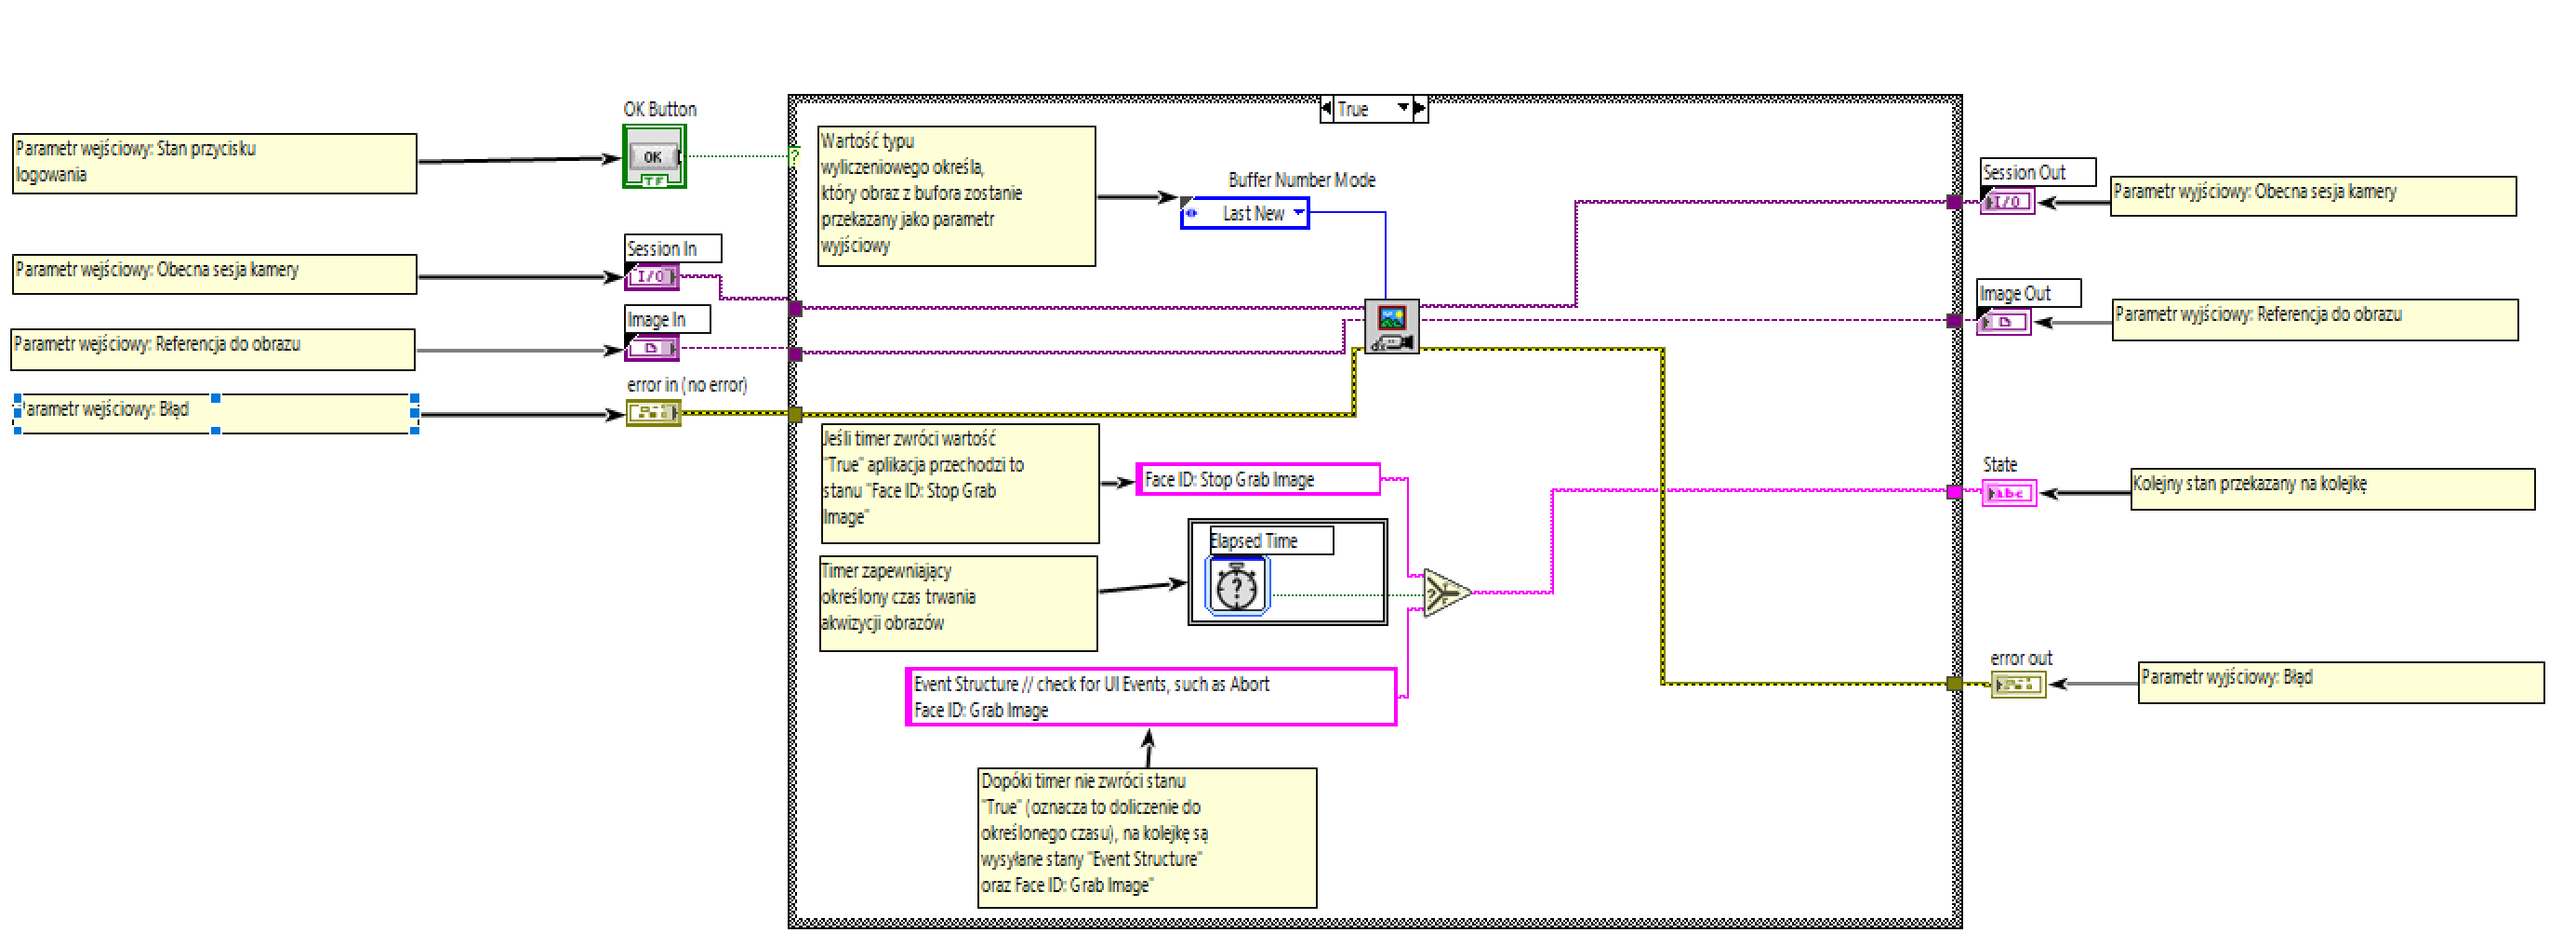
\includegraphics[width=1.0\textwidth]{src/face-id/face-id-case.png}
    \caption{Zdjęcie przedstawiające SubVI Take Image Case Struct w przypadku stanu wysokiego odebranego z przycisku}
    \label{fig:face_id-grab-case}
\end{figure}

\begin{figure}[H]
    \centering
    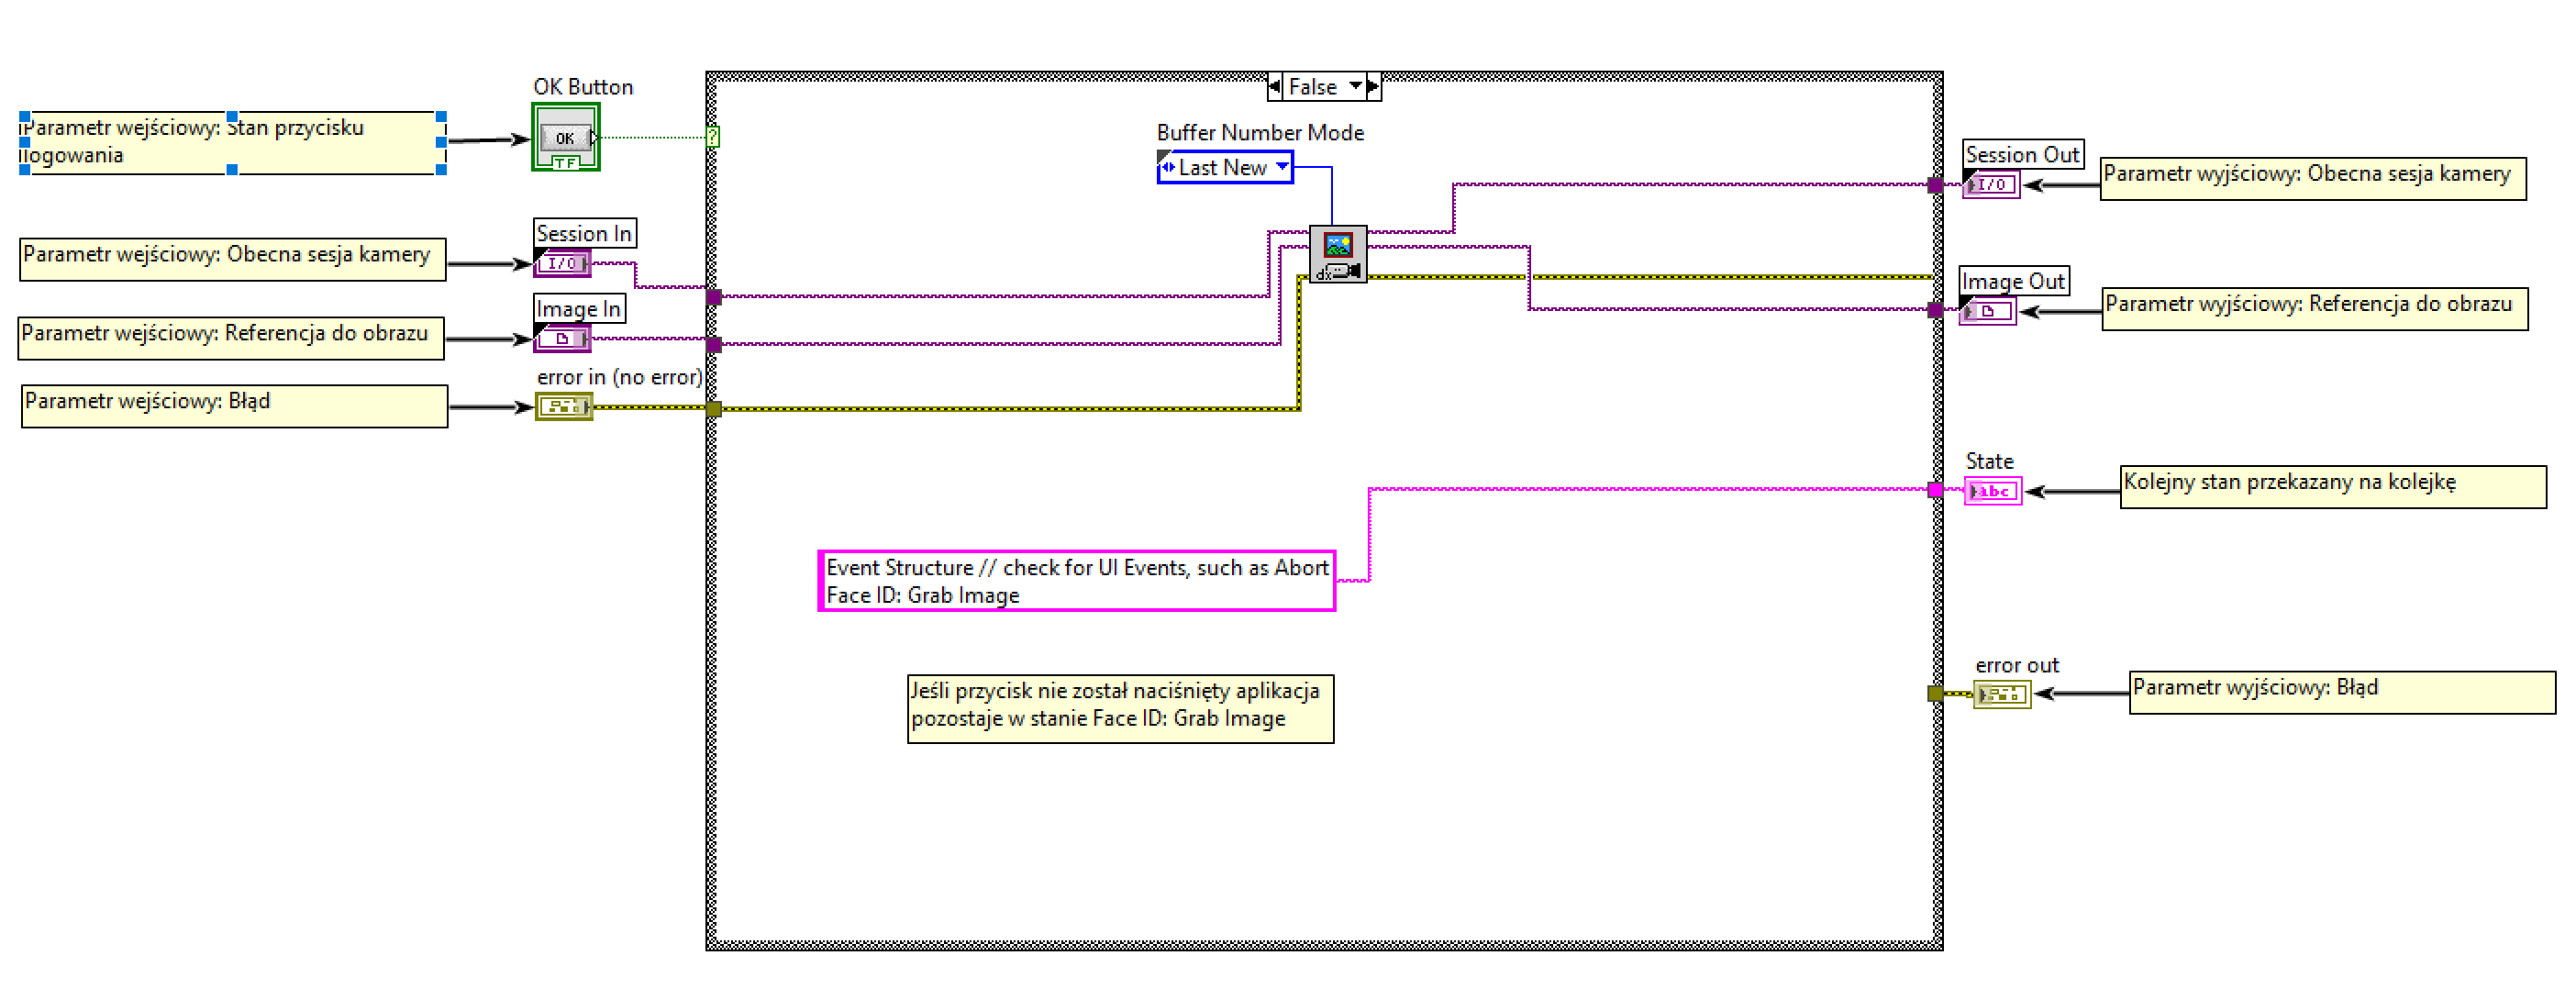
\includegraphics[width=1.0\textwidth]{src/face-id/face-id-case-2.png}
    \caption{Zdjęcie przedstawiające SubVI Take Image Case Struct w przypadku braku sygnału z przycisku}
    \label{fig:face_id-grab-case-2}
\end{figure}

\subsubsection{\large Stan Face ID: Stop Grab Image}

Następny stan odpowiada za zatrzymanie akwizycji obrazu oraz usunięcie nieużywanych referencji w celu zwolnienia zasobów komputera.

Pierwszą wykonywaną funkcją jest wyodrębnienie danych z klastra pochodzącego z linii danych. Następnie, trwająca sesja kamery zostaje przekazana jako parametr wejściowy dla bloku "Stop Acquisition". Sesja kamery jest następnie przekazywana do bloków "Unconfigure Camera" oraz "Close Camera". Ta sekwencja jest konieczna do poprawnego zamknięcia kamery. Jeśli nie wszystkie kroki zostaną wykonane, istnieje ryzyko, że kamera będzie niewidoczna lub niedostępna dla innych aplikacji z powodu nieusuniętej referencji utworzonej przez aplikację LabVIEW.

Referencja do obrazu zostaje przekazana do bloku "Save Image". Zapis obrazu jest konieczny ze względu na późniejszą analizę zarejestrowanego obrazu oraz weryfikację tożsamości. Następnie referencja jest usuwana przy użyciu bloku "Imaq Dispose".

Warto zauważyć sposób przekazania ścieżki do zapisu zarejestrowanego obrazu. W celu większej elastyczności programu zastosowane zostały ścieżki względne. Budowa ścieżki względnej rozpoczyna się od użycia bloku "Current VI's Path", zwracającego ścieżkę bezwzględną do aktualnej lokalizacji VI. Następnie odpowiednio dodawana jest stała typu "Path Constant", w taki sposób, aby otrzymać pożądaną lokalizację. Następnie używany jest blok "Build Path", który konkatenuje obie składowe, tworząc poprawną ścieżkę.

Do linii danych przekazywana jest pusta referencja do sesji kamery, przygotowując system na ewentualne ponowne użycie kamery. Do kolejki przekazywany jest kolejny stan "Face ID: Image Processing".

Ponieważ niebezpieczeństwo zablokowania aplikacji podczas używania kamery przestaje obowiązywać po jej zamknięciu, zostaje włączony domyślny timeout.

Dodatkowo, następuje przejście z zakładki "Page 1" do zakładki "Page 2" za pomocą bloku "Tab Control", do którego na wejście przekazywana jest odpowiednia wartość typu wyliczeniowego zawierającego istniejące zakładki.


\begin{figure}[H]
    \centering
    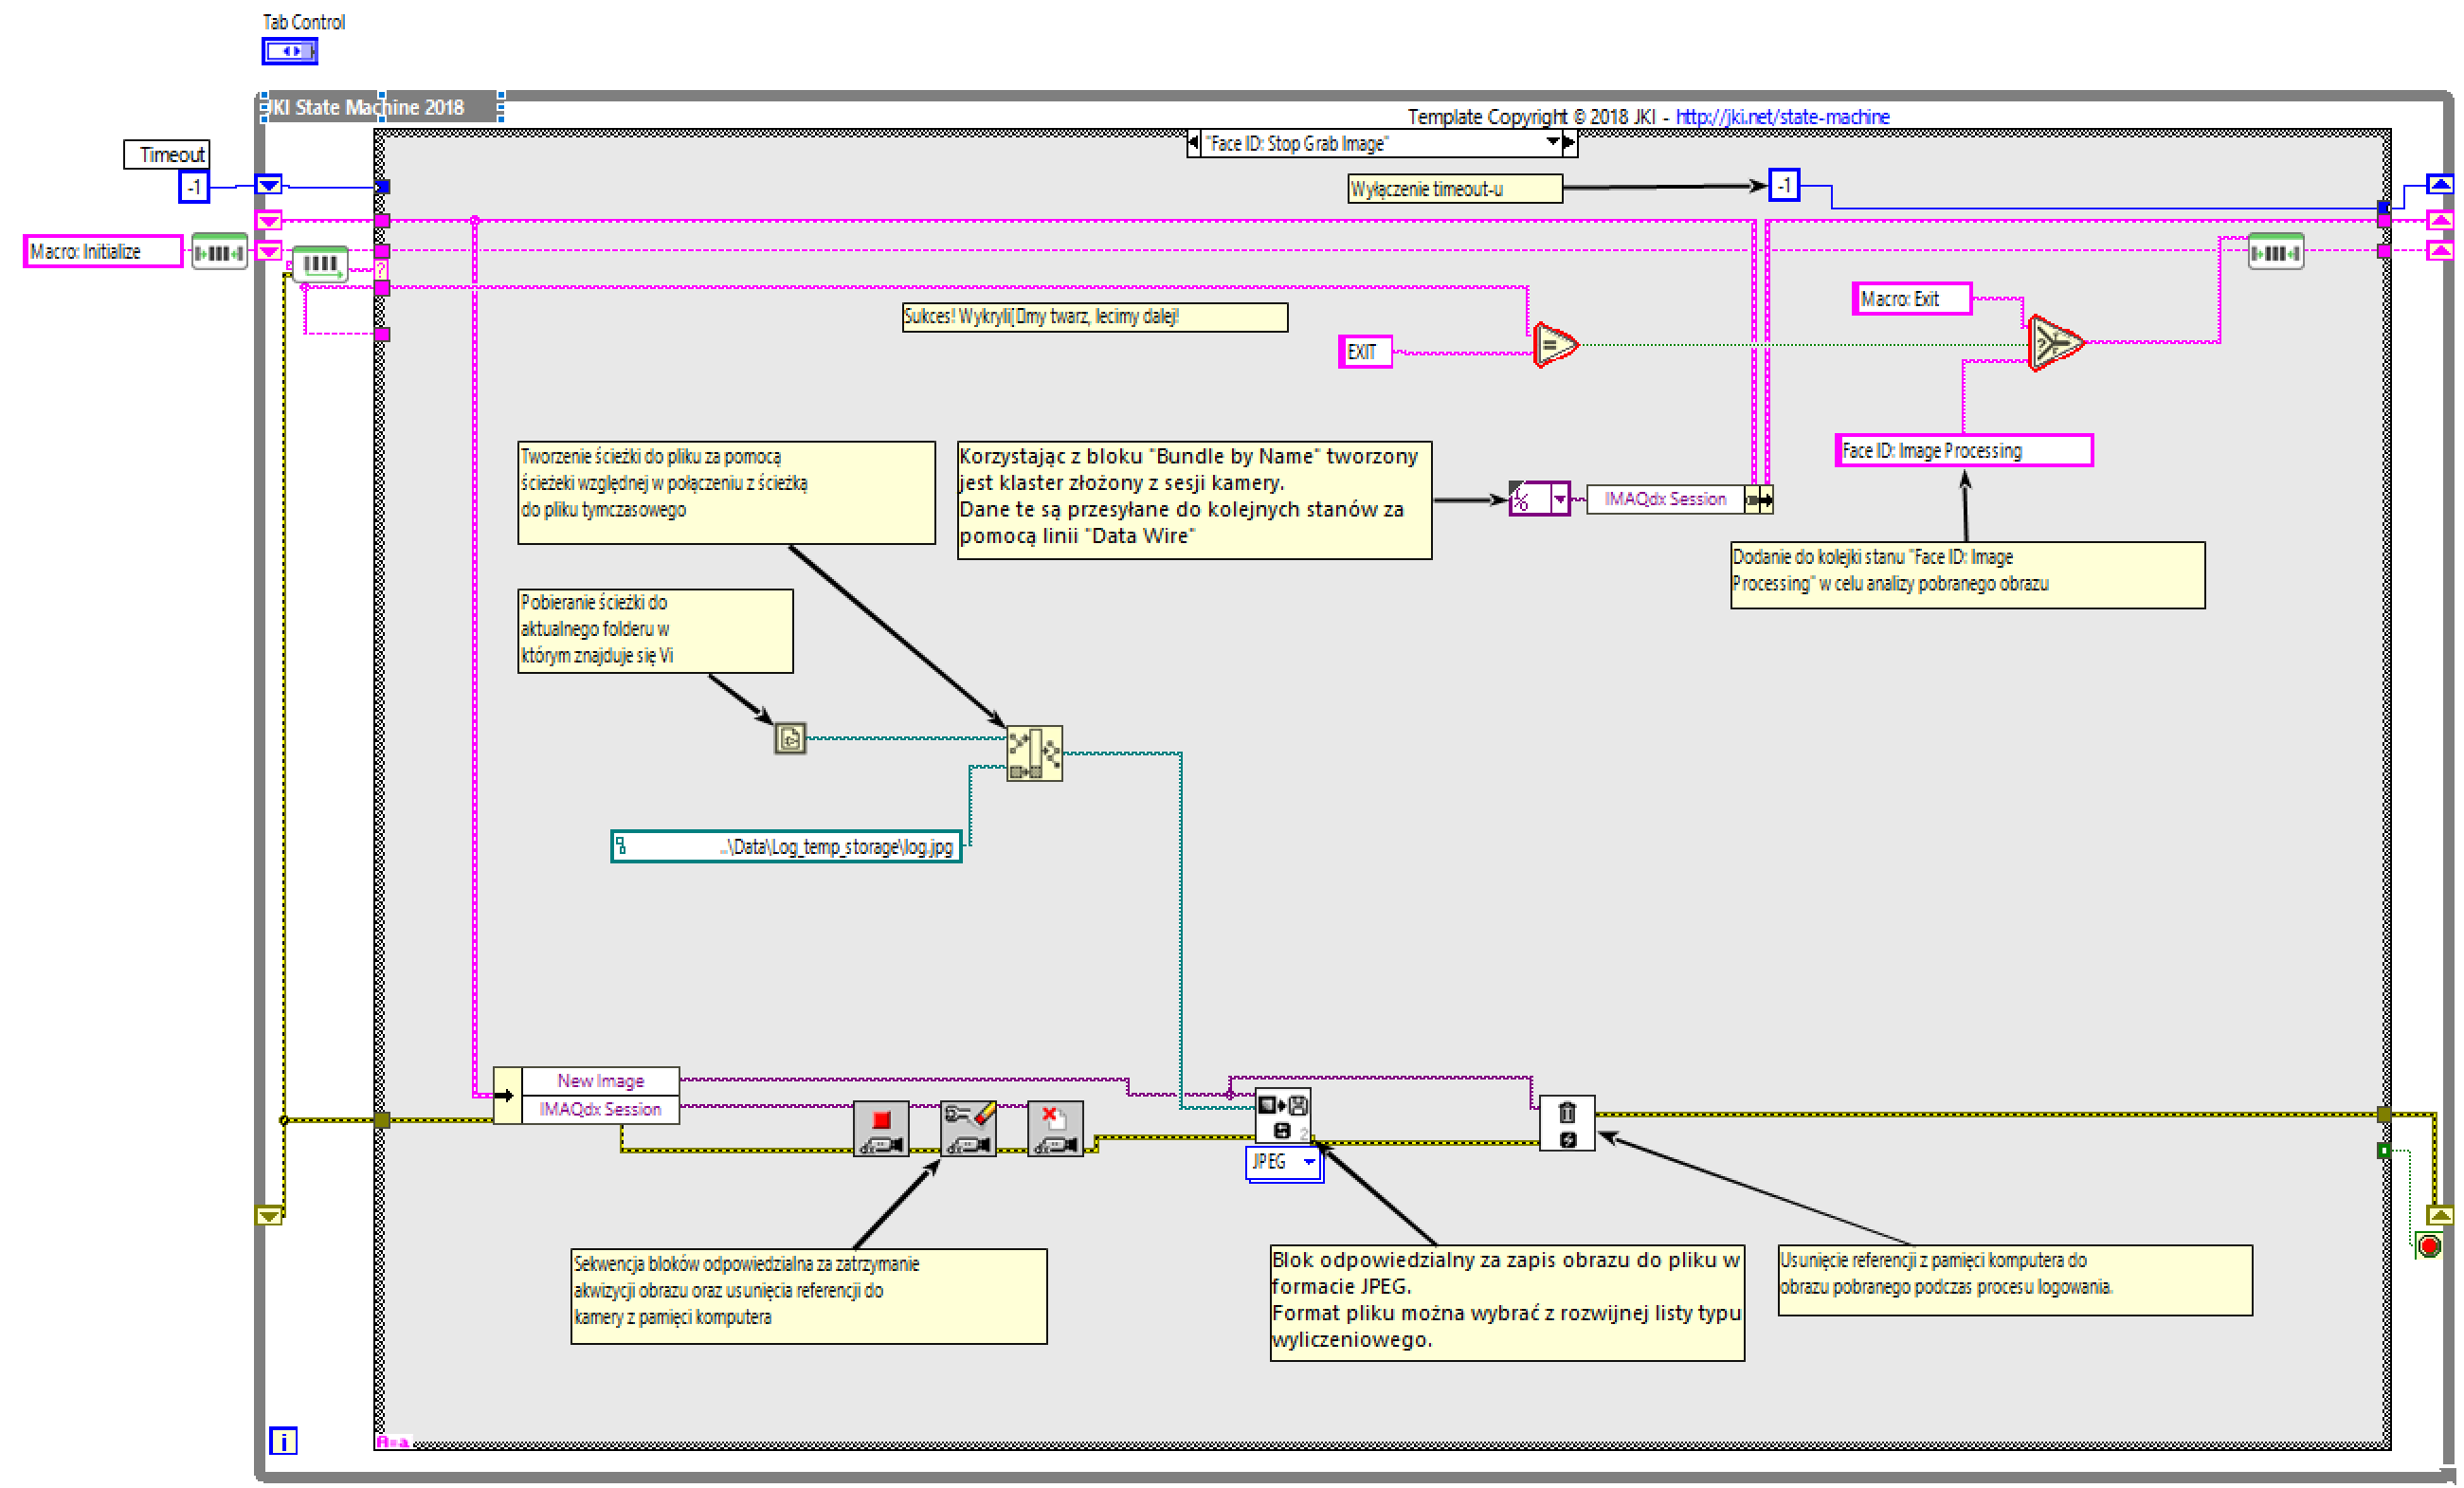
\includegraphics[width=1.0\textwidth]{src/face-id/face-id-stop-grab.png}
    \caption{Zdjęcie przedstawiające stan Face ID: Stop Grab Image}
    \label{fig:face_id-stop-grab}
\end{figure}

\subsubsection{\large Stan Face ID: Image Processing}

Ostatni stan związany z procesem logowania to "Face ID: Image Processing". Proces identyfikacji użytkownika rozpoczyna się od bloku "Open Python Session", który przygotowuje środowisko uruchomieniowe LabVIEW do użycia języka Python. Na wejście bloku należy podać błąd, wersję języka Python oraz ścieżkę do pliku wykonywalnego .exe uruchamiającego kompilator. Na wyjściu pojawi się sygnał zawierający aktualną sesję Python oraz ewentualny błąd.

Następnie następuje właściwe wywołanie funkcji realizującej porównanie. Na wejście bloku "Python Node" należy podłączyć otwartą wcześniej sesję oraz ścieżkę do miejsca, w którym znajduje się skrypt. Ścieżka została zaimplementowana za pomocą bloku "Path Builder". Opcjonalnie blok "Python Node" można rozciągnąć, aby pokazały się puste pola, które obrazują argumenty wejściowe funkcji oraz typ wartości zwracanej. W aktualnej wersji aplikacji do wymienionego bloku została podłączona stała typu Boolean, co wskazuje na typ wartości zwracanej. Argumenty wejściowe nie są wymagane w obecnej wersji aplikacji.

Po zakończeniu działania sesja Python zostaje zamknięta, a wartość zwrócona z funkcji \newline \texttt{find\_face\_encodings} wywołuje odpowiedni stan struktury case. Jeśli proces logowania został zakończony sukcesem, wykonuje się case "True" - wyświetlana jest informacja na ekranie użytkownika o statusie logowania, a do kolejki zostaje przekazany kolejny stan, którym jest "Face ID: Control Panel". Następuje również przełączenie na trzecią zakładkę za pomocą bloku "Tab Control".

W przypadku, gdy logowanie nie zakończyło się sukcesem, wyświetlana jest informacja o statusie logowania, a do kolejki zostaje przekazany stan "Face ID: Initialize Grab Image", co powoduje, że aplikacja wraca do stanu początkowego. Zakładka zostaje przełączona na ekran początkowy.
 

\begin{figure}[H]
    \centering
    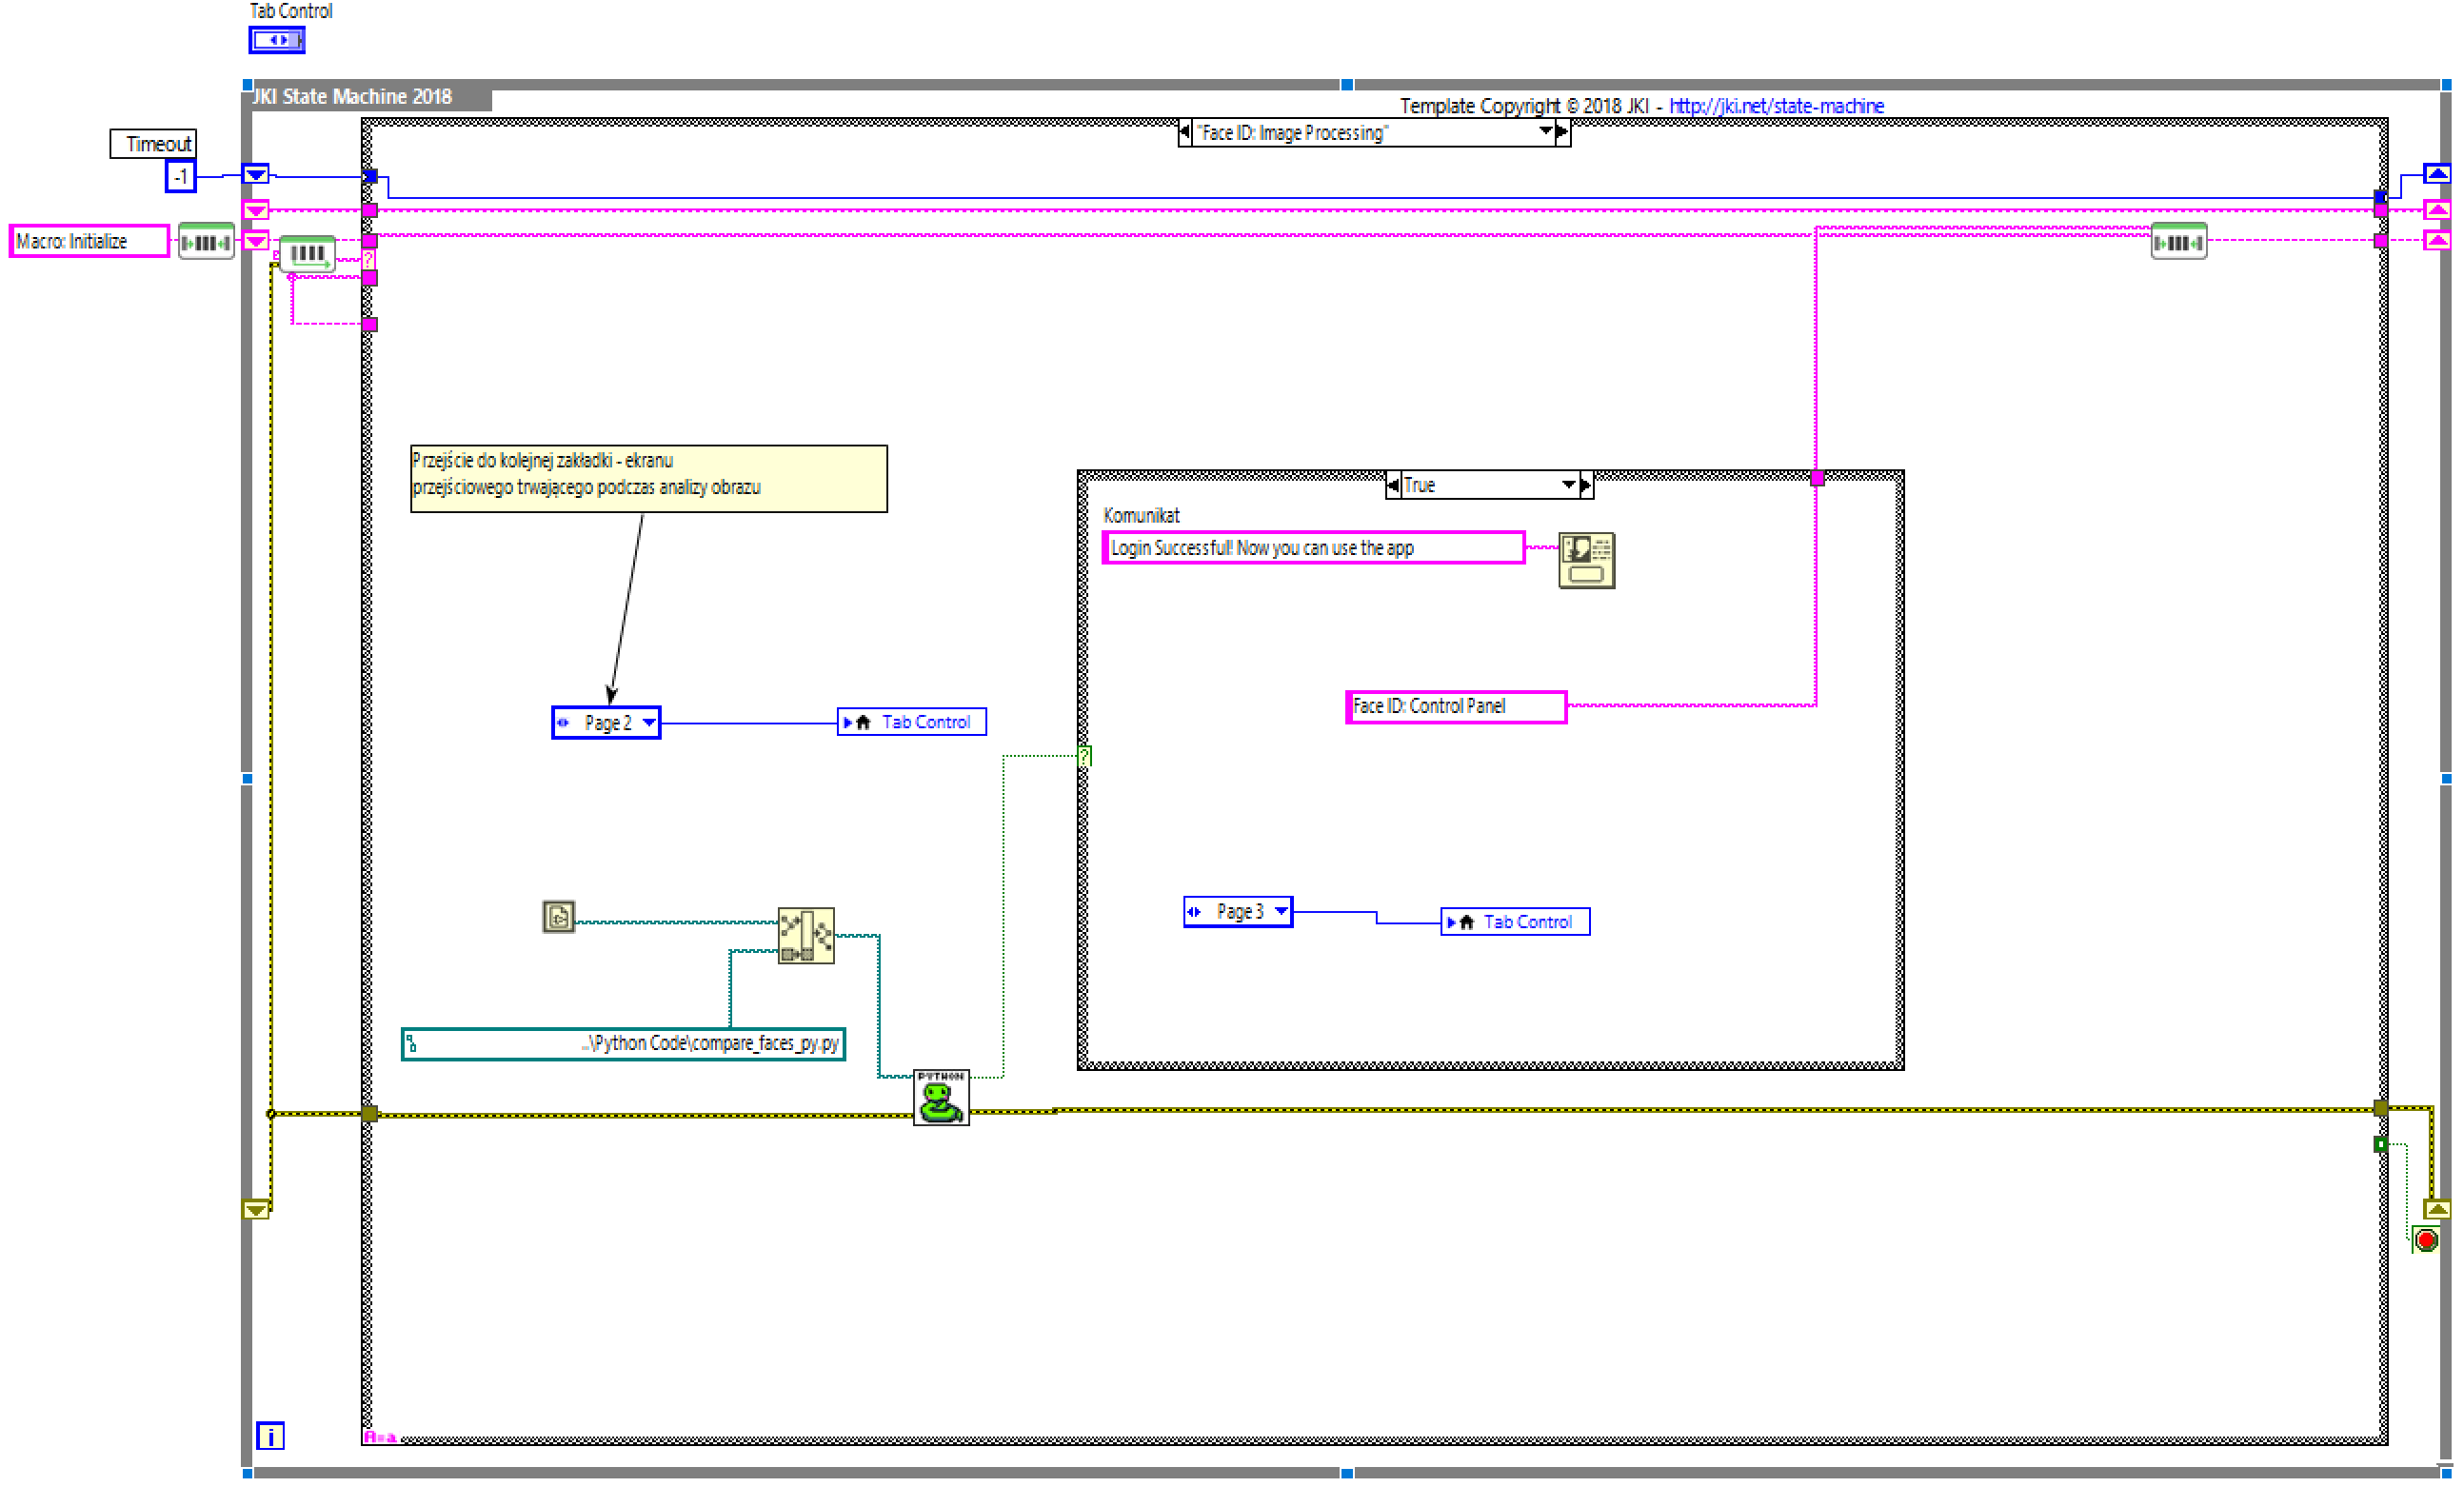
\includegraphics[width=1.0\textwidth]{src/face-id/face-id-image-process.png}
    \caption{Zdjęcie przedstawiające stan Face ID: Image Processing jeśli logowanie zakończyło się sukcesem}
    \label{fig:face_id-process}
\end{figure}

\begin{figure}[H]
    \centering
    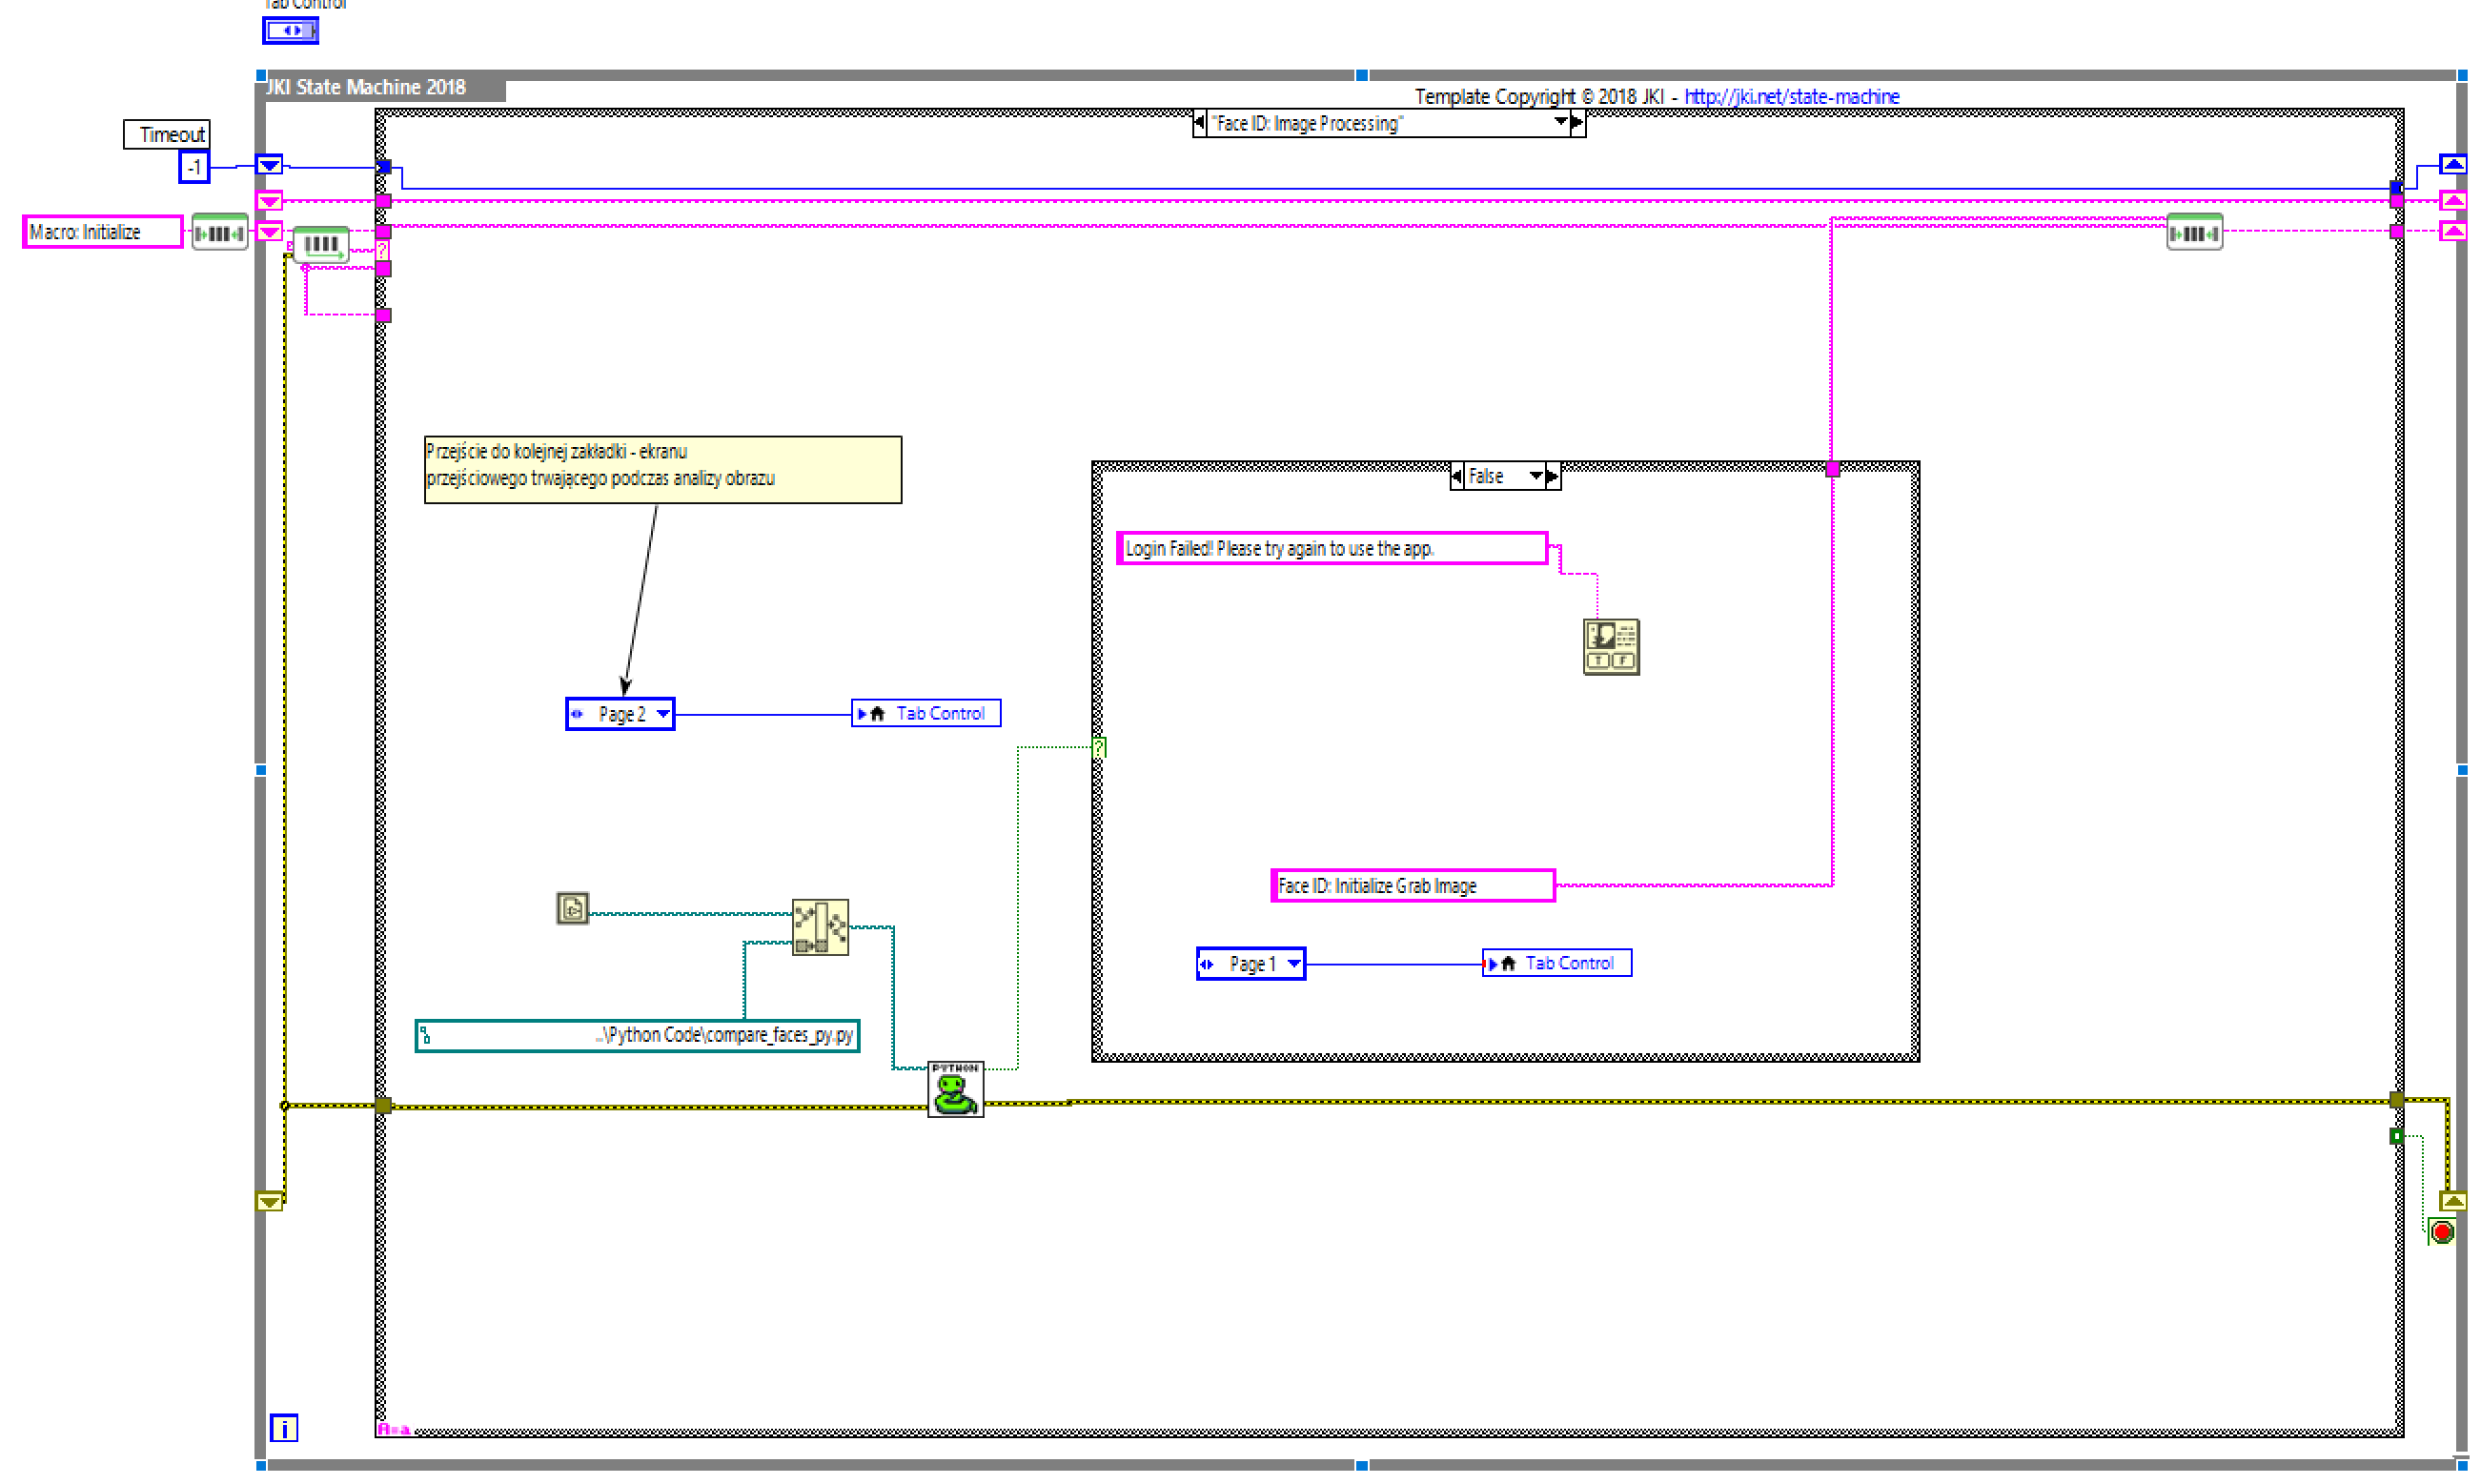
\includegraphics[width=1.0\textwidth]{src/face-id/face-id-image-process-2.png}
    \caption{Zdjęcie przedstawiające stan Face ID: Image Processing jeśli logowanie zakończyło się niepowodzeniem}
    \label{fig:face_id-process-2}
\end{figure}

\subsection{\Large Implementacja identyfikacji użytkownika}

Funkcja \texttt{find\_face\_encodings} realizuje proces porównania twarzy w celu identyfikacji użytkownika. Działanie funkcji można podzielić na kilka kluczowych kroków.

Na początku, funkcja definiuje ścieżkę do folderu z zarejestrowanymi użytkownikami oraz wczytuje tymczasowy obraz logowania za pomocą biblioteki \texttt{cv2}. 

Następnie, za pomocą funkcji \texttt{face\_recognition.face\_encodings}, funkcja przetwarza wczytany obraz w celu ekstrakcji cech twarzy. Jeżeli w obrazie nie zostanie wykryta twarz, funkcja zwraca wartość \texttt{False} i kończy działanie, informując o braku wykrycia twarzy.

Funkcja iteruje przez wszystkie pliki graficzne znajdujące się w folderze z zarejestrowanymi użytkownikami. Dla każdego obrazu próbuje wyodrębnić cechy twarzy. Jeżeli w obrazie nie zostanie wykryta twarz, funkcja kontynuuje przetwarzanie kolejnych plików, informując o niepowodzeniu detekcji dla danego pliku.

Dla każdej zarejestrowanej twarzy, funkcja porównuje jej kodowanie z kodowaniem twarzy z obrazu logowania za pomocą funkcji \texttt{face\_recognition.compare\_faces}. Jeżeli zostanie znalezione dopasowanie, funkcja oblicza odległość pomiędzy kodowaniami twarzy przy użyciu funkcji \newline \texttt{face\_recognition.face\_distance} oraz przekształca tę odległość na poziom dokładności (accuracy).

Jeżeli funkcja znajdzie dopasowanie, informuje o sukcesie porównania, wyświetlając nazwę dopasowanego pliku oraz poziom dokładności. Funkcja zwraca wartość \texttt{True}, sygnalizując pomyślne logowanie użytkownika. 

Jeżeli żadne z kodowań twarzy z zarejestrowanych obrazów nie będzie zgodne z kodowaniem twarzy z obrazu logowania, funkcja zwraca wartość \texttt{False}, informując o niepowodzeniu procesu logowania.

Funkcja \texttt{find\_face\_encodings} jest kluczowym elementem systemu rozpoznawania twarzy, odpowiadającym za porównanie twarzy użytkownika z bazą zarejestrowanych obrazów. Wykorzystując biblioteki \texttt{cv2} oraz \texttt{face\_recognition}, funkcja ta skutecznie identyfikuje użytkownika, zapewniając odpowiedni poziom dokładności i niezawodności.

% \begin{figure}
%     \centering
%     \includegraphics*[keyvals]{imagefile}
%     \caption{Kod źródłowy realizujący weryfikację tożsamości użytkownika}
%     \label{fig:python-code}
% \end{figure}

\subsection{\Large Implementacja procesu dodawania użytkownika}

\subsubsection{\large Stan Add User: Input Image Init}

Pierwszym elementem dodania nowego użytkownika do bazy danych znanych użytkowników jest inicjalizacja kamery. Stan ten jest bliźniaczo podobny do stanu Face ID: Grab Image Init, dlatego też nie będzie ponownie szczegółowo opisywany. 

\begin{figure}[H]
    \centering
    \includegraphics*[width=1.0\textwidth]{src/add-user/add-init.png}
    \caption{Obraz przedstawiający schemats blokowy realizujący inicjalizację kamery}
    \label{fig:add-user-init}
\end{figure}

\subsubsection{\large Stan Add User: Grab Input Image}

Logika oraz zasada działania stanu "Add User: Grab Image" są niemal identyczne jak w przypadku stanu "Face ID: Grab Image". Kluczową różnicą jest wprowadzenie nowego elementu do linii danych \textit{Data Wire}, nazwanego \textit{"Img Path"}. Jest to parametr typu \texttt{String}, który określa nazwę pliku (tu: zdjęcia) uzyskanego podczas procesu dodawania nowego użytkownika.

Nazwa pliku jest generowana poprzez konkatenację dwóch zmiennych typu \texttt{String} oraz jednej stałej typu \texttt{String}. Zmienne te pochodzą z panelu użytkownika, gdzie przed rozpoczęciem akwizycji obrazu użytkownik wprowadza swoje imię i nazwisko. Te dwa parametry tworzą główną część nazwy pliku. Ostatnia składowa jest stałą określającą rozszerzenie pliku. Ze względu na relatywnie niewielki rozmiar, użyto rozszerzenia \textit{.jpg}.

Konkatenacja trzech ciągów znaków jest realizowana za pomocą bloku \textit{Concatenate Strings}, dostępnego w standardzie LabVIEW.

Różnica występuje również w sposobie przekazania kolejnego stanu do kolejki. Z uwagi na pierwotne napisanie pakietu \textit{SubVI} dla stanu \textit{"Face ID: Grab Image"}, blok na wyjściu przekazuje kolejny stan kategorii \textit{Face ID}. Aby uniknąć powielania kodu, zastosowano metodę porównania oraz selektor, który na podstawie wyniku porównania dodaje do kolejki odpowiednie stany.

Jeśli blok zwróci stan \textit{"Face ID: Stop Grab Image"}, podczas operacji porównania zostanie zwrócona wartość \texttt{True}, co wpłynie na selektor, który doda do kolejki stan \textit{"Add User: Stop Grab Image"}.

\begin{figure}[H]
    \centering
    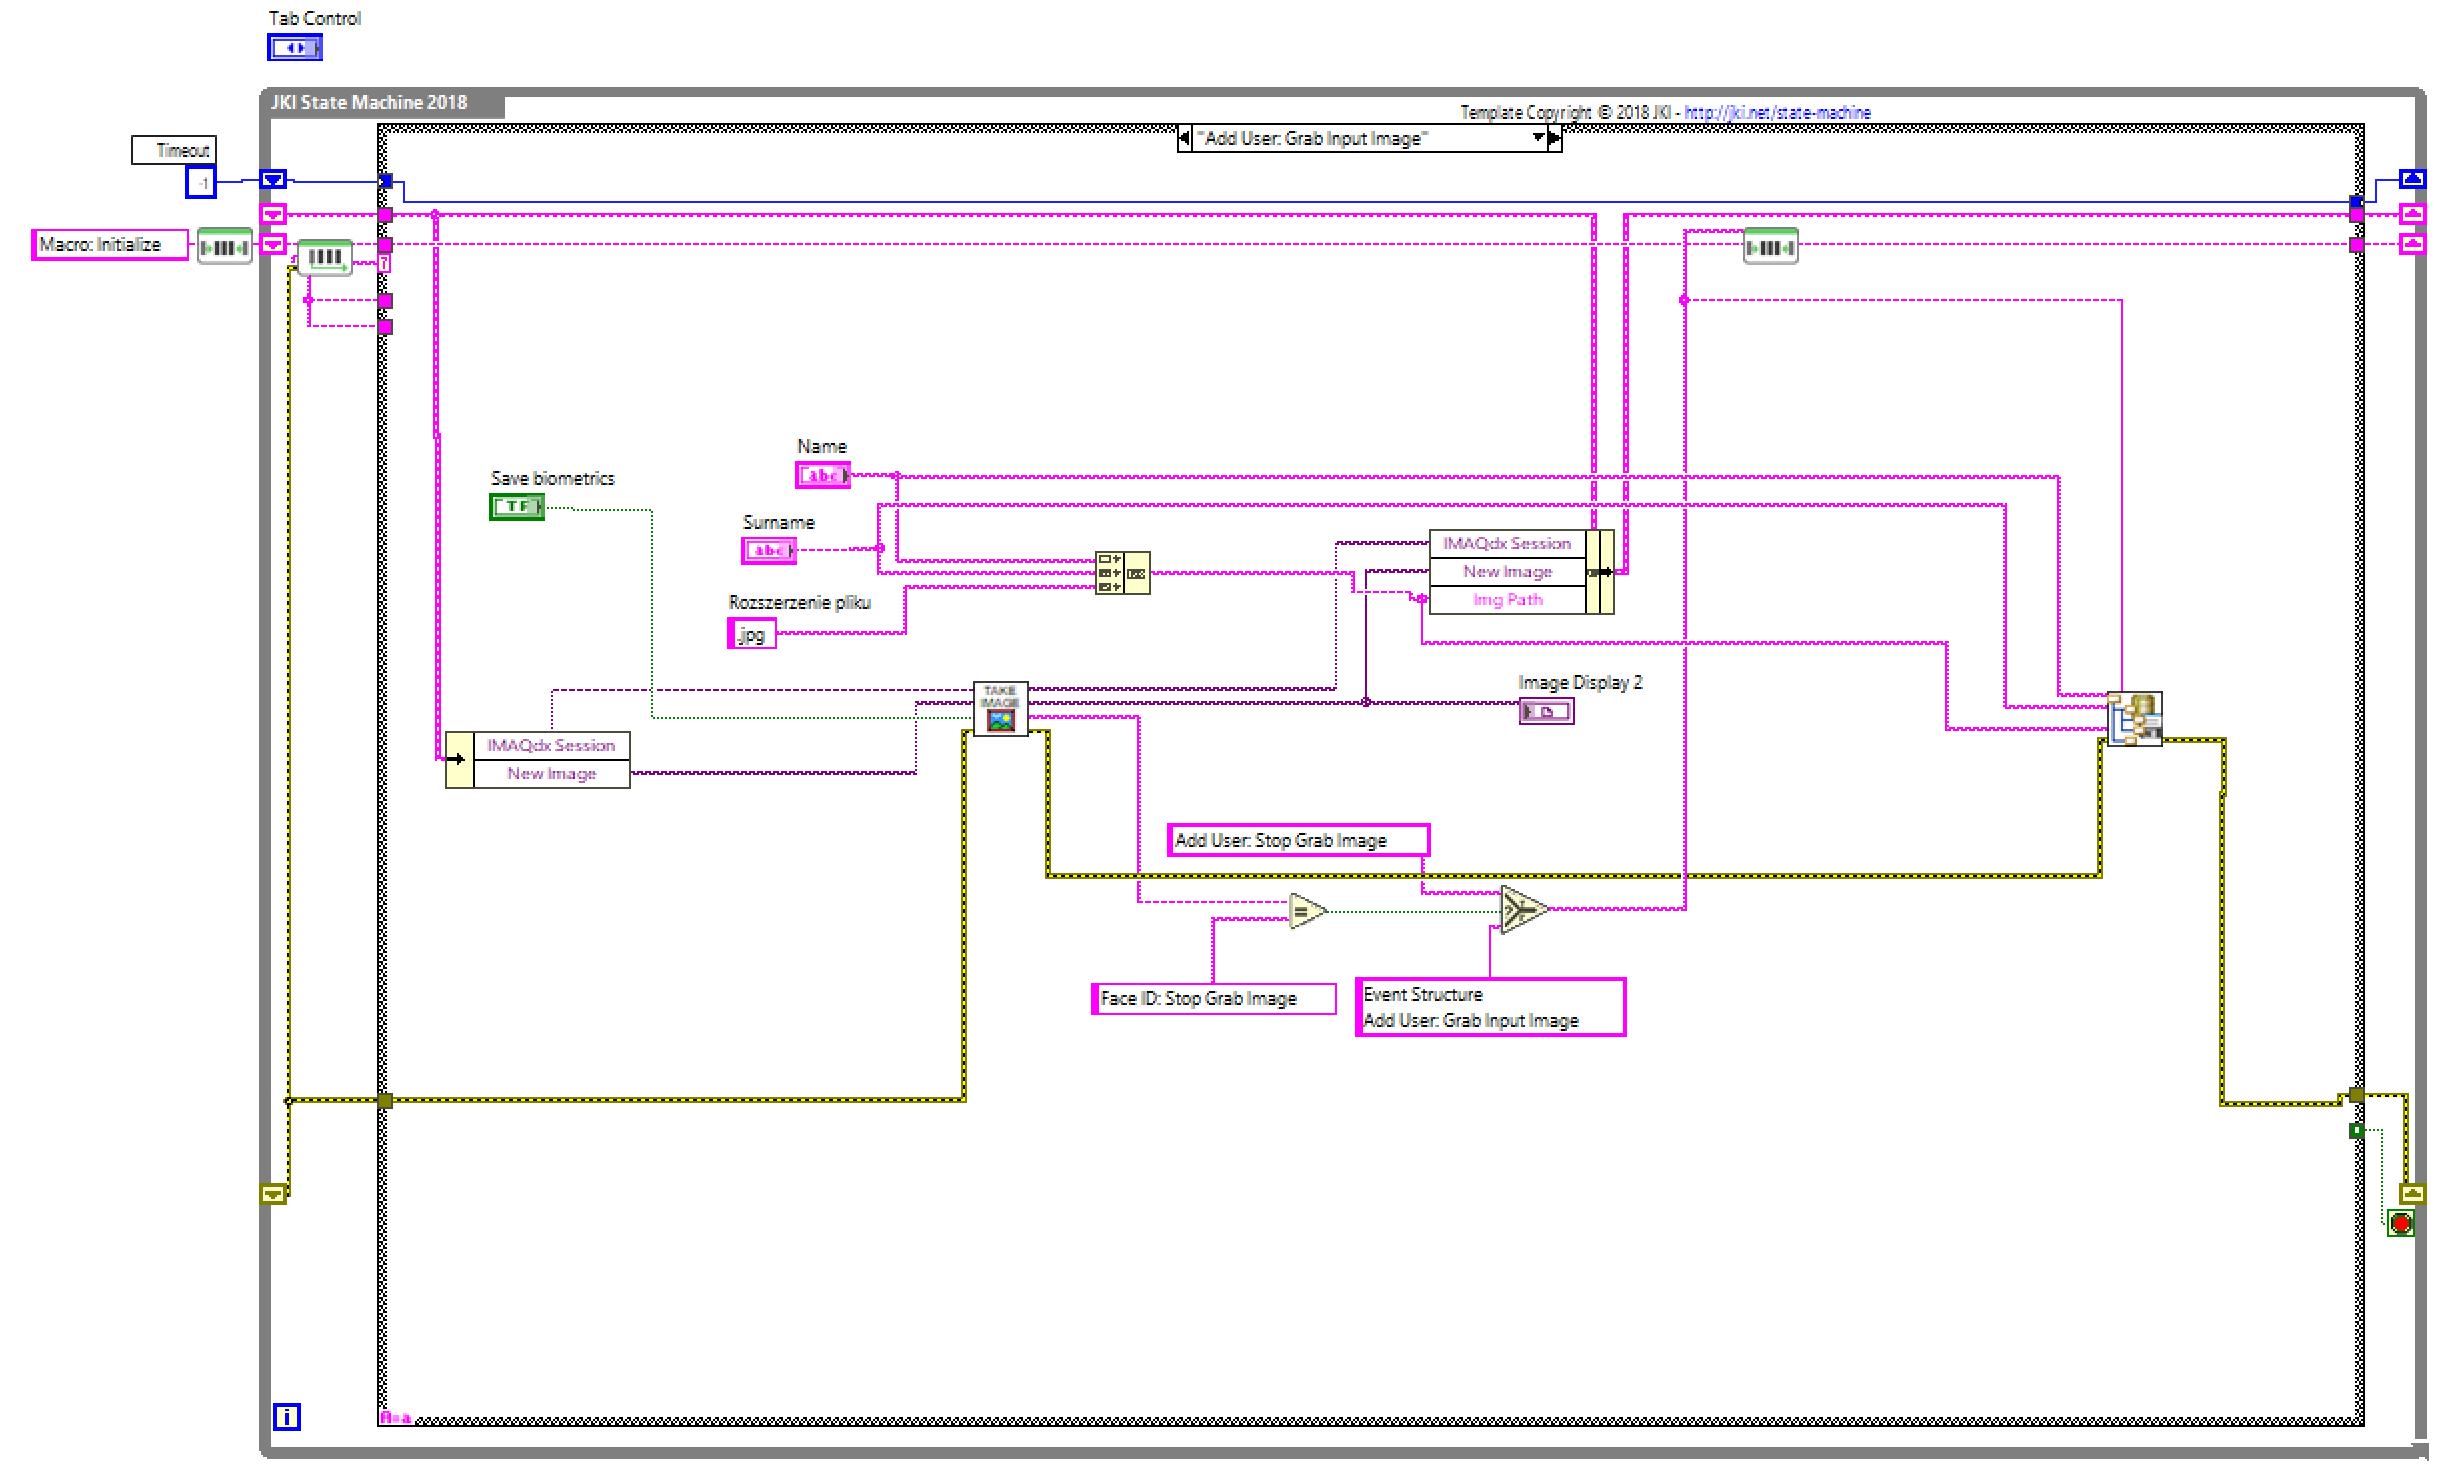
\includegraphics[width=1.0\textwidth]{src/add-user/add-grab.png}
    \caption{Obraz przedstawiający stan Add User: Grab Input Image}
    \label{fig:add-user-grab}
\end{figure}

\subsubsection{\large Stan Add User: Stop Grab Image}


Stan ten jest zbliżony do stanu \textit{Face ID: Stop Grab Image}, z tą różnicą, że do kolejki przekazywany jest inny stan, mianowicie \textit{Face ID: Control Panel}, zamiast stanu \textit{Face ID: Image Processing}. Jest to spowodowane koniecznością uniknięcia weryfikacji tożsamości podczas dodawania nowego użytkownika, co byłoby nielogiczne.

Podczas tego stanu, proces zapisu pliku został zmodyfikowany w zakresie parametrów ścieżki do pliku. W przypadku logowania, bieżące pliki są zapisywane w folderze \textit{Log\_temp\_storage}. Natomiast pliki pobrane podczas dodawania nowego użytkownika są zapisywane w folderze \textit{Registered\_Users} pod nazwą pobraną z linii danych \textit{Data Wire}.

Warto podkreślić użycie bloku \textit{String to Path}, który jest dostarczany w standardzie LabVIEW. Blok ten przekształca typ \textit{String} na typ \textit{Path}, co zapewnia zgodność typu zmiennej przekazywanej na wejście bloku \textit{Path Builder} z oczekiwanym typem.


\begin{figure}[H]
    \centering
    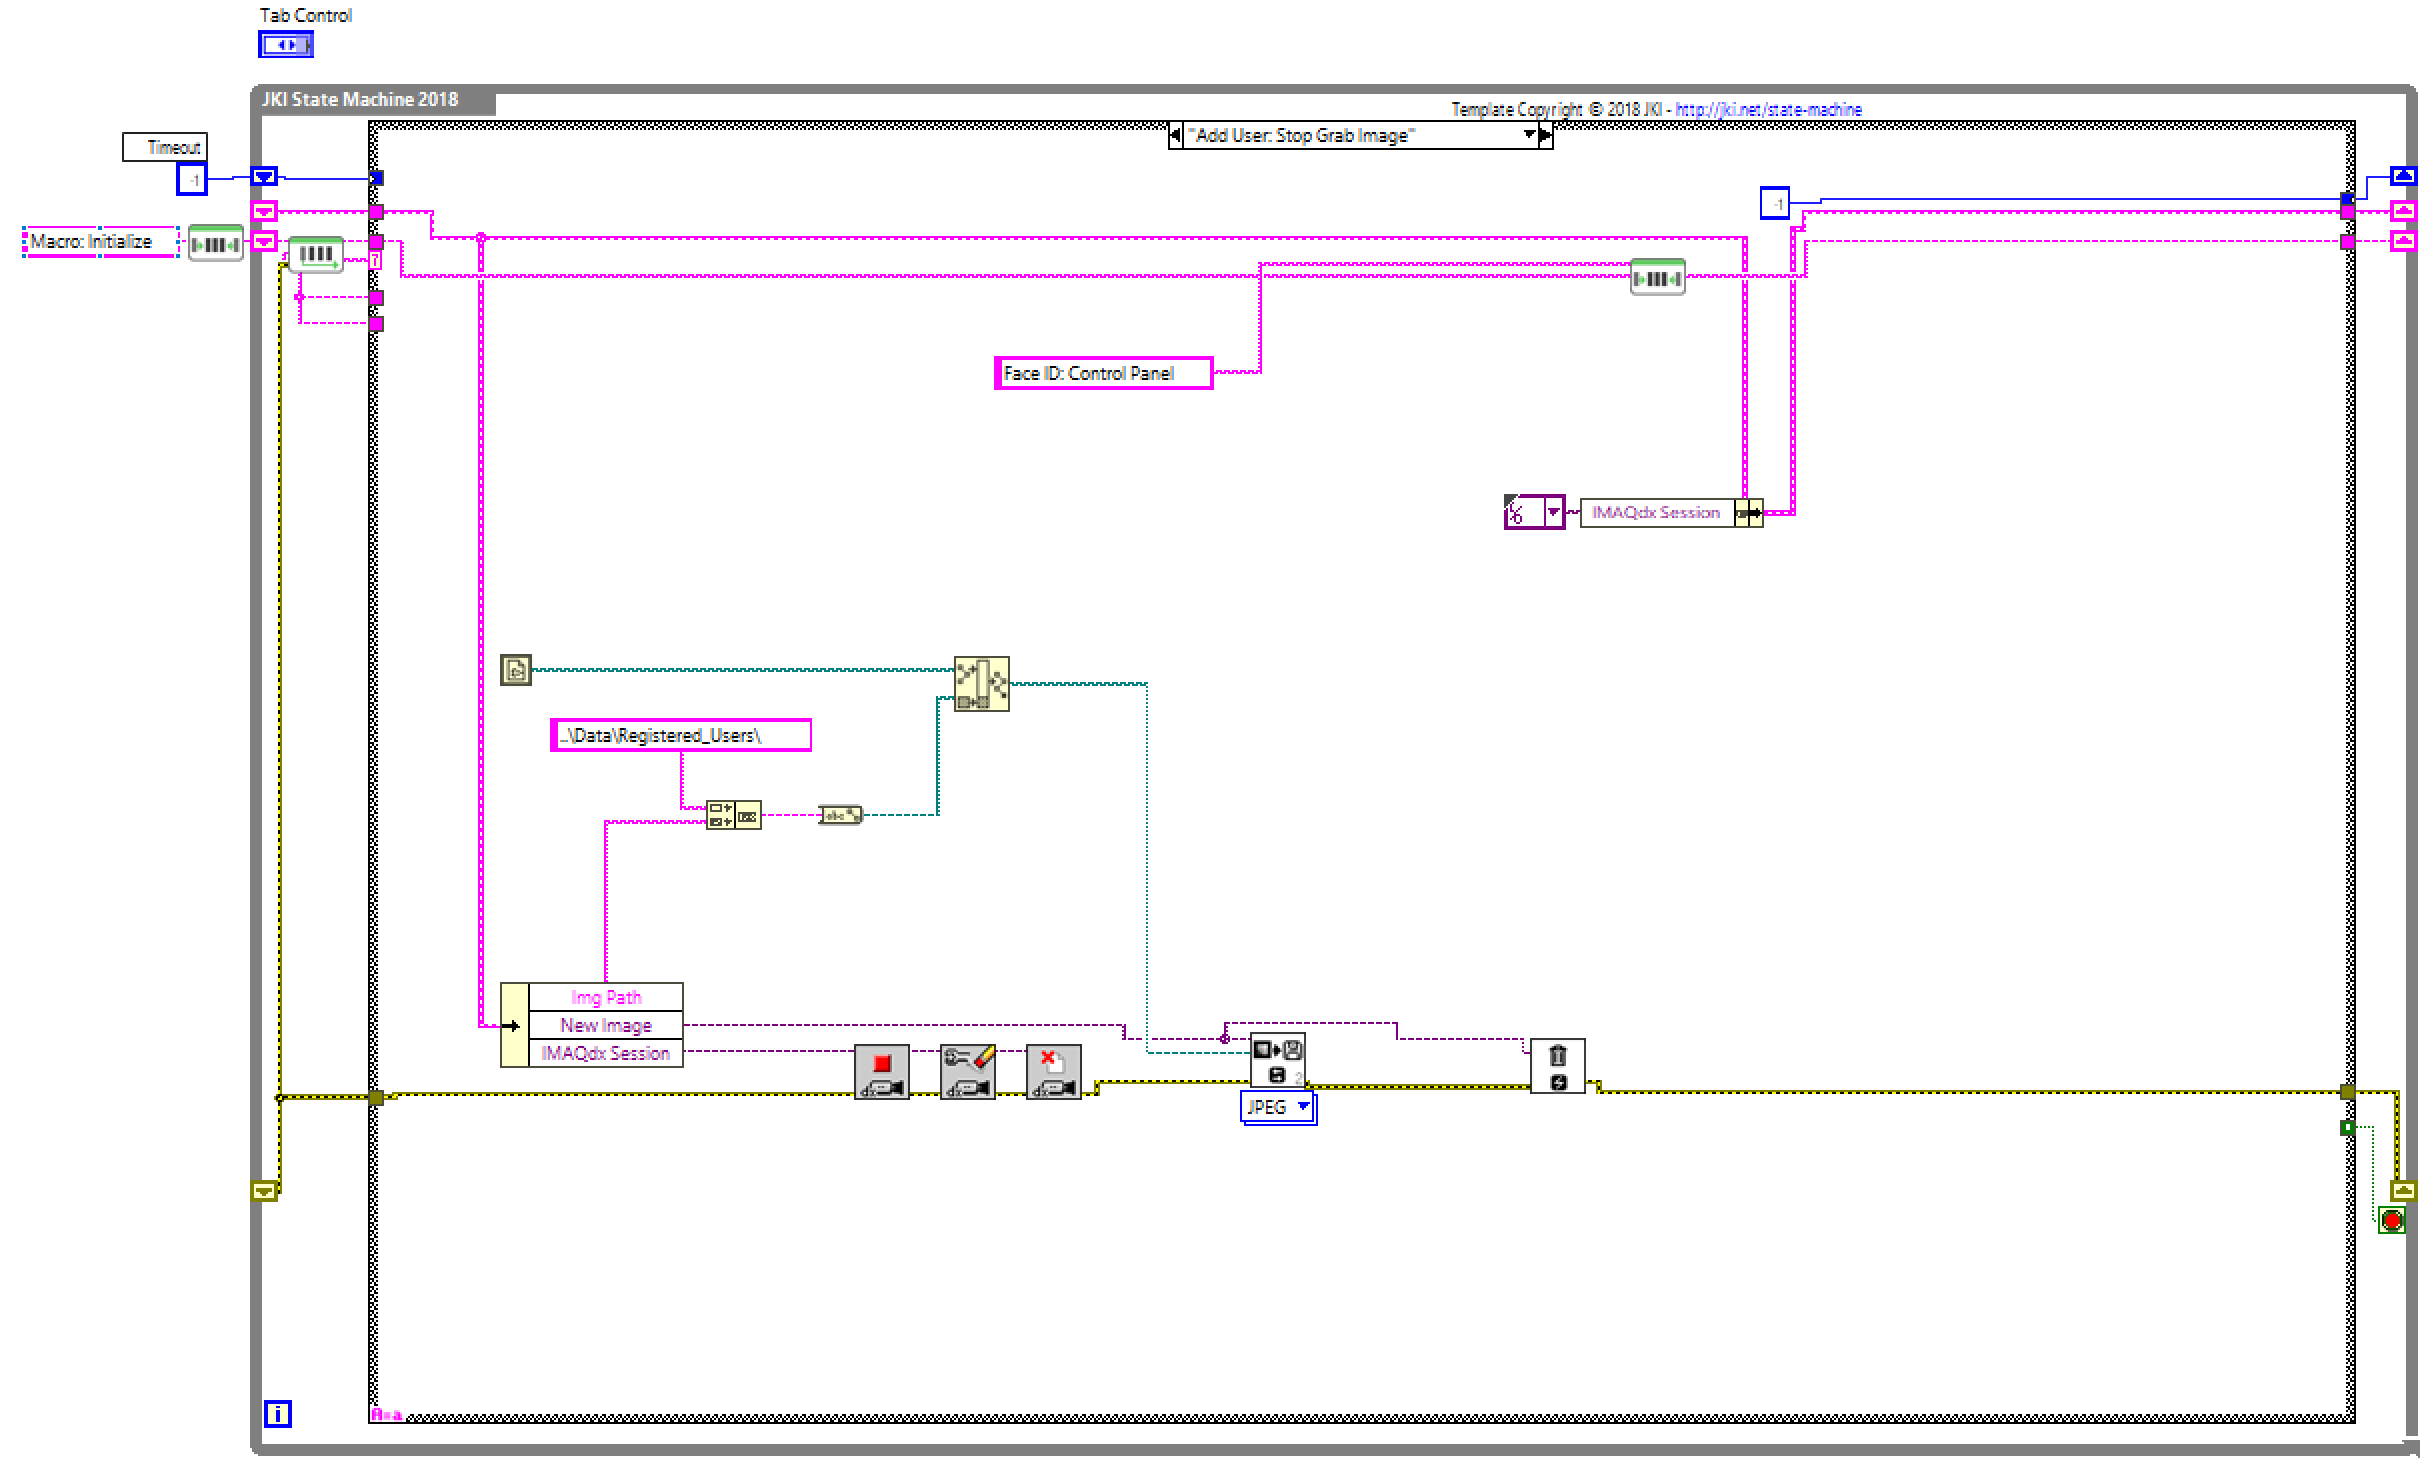
\includegraphics[width=1.0\textwidth]{src/add-user/add-stop.png}
    \caption{Obraz przedstawiający stan Add User: Stop Grab Image}
\end{figure}

\subsection{\Large Implementacja połączenia aplikacji z bazą danych}

% --------------------------------------------------------
% Autor: Łukasz Grabarski, Jakub Pająk
%
% TODO: Opisać proces działającego połączenia z bazą danych SQL Server
%
% Status: Łukasz 100%
% --------------------------------------------------------
W celu poprawnego funkcjonowania aplikcji, niezbędnym było utworzenie tabeli w bazie danych. Do tego celu został wykorzystany program 
Microsoft SQL Server Management Studio. Tabela ma za zadanie przechowywać takie dane użytkownika jak \textit{Imię, Nazwisko, Input, Nazwa pliku}.
Input jest wartością zdolną do modyfikacji w aplikacji, ponieważ owa kolumna ma służyć do prostej obsługi konta indywidualnie dla każdego użytkownika.
Kolumna Nazwa pliku przechowuje ścieżkę względną do obrazu referencyjnego, który jest wykorzystywany przez skrypt w Pythonie do zidentyfikowania danej
osoby próbującej się zalogować.

\begin{figure}[H]
    \centering
    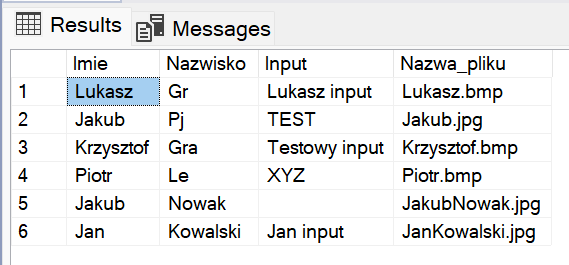
\includegraphics[width=0.6\textwidth]{src/Database/Microsoft SQL.png}
    \caption{Obraz przedstawiający tablicę wynikową bazy danych utworzonej w Microsoft SQL Server Management Studio. Wiersze 5-6 zostały dodane za pomocą aplikacji LabView.}
    \label{fig:first-att}
\end{figure}


\subsubsection{\large Generowanie linku do bazy danych}

\begin{figure}[H]
    \centering
    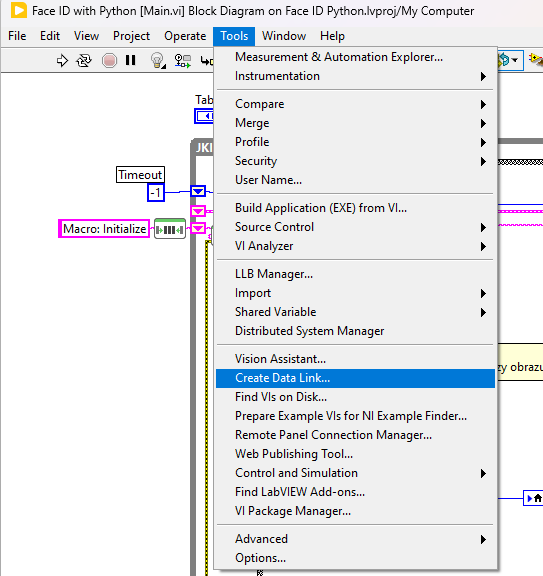
\includegraphics[width=0.6\textwidth]{src/Database/Stage1.png}
    \caption{Rozwinięcie listy Tools i wybranie pozycji Create Data Link}
    \label{fig:first-att}
\end{figure}

\begin{figure}[H]
    \centering
    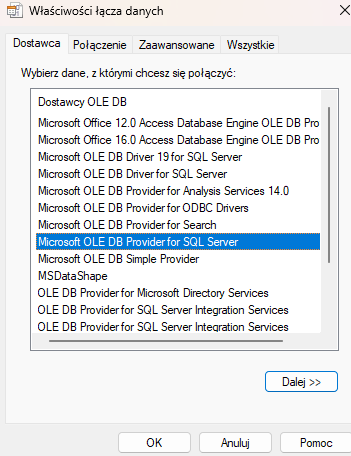
\includegraphics[width=0.6\textwidth]{src/Database/Stage2.png}
    \caption{Wybór odpowiednich danych}
    \label{fig:first-att}
\end{figure}

\begin{figure}[H]
    \centering
    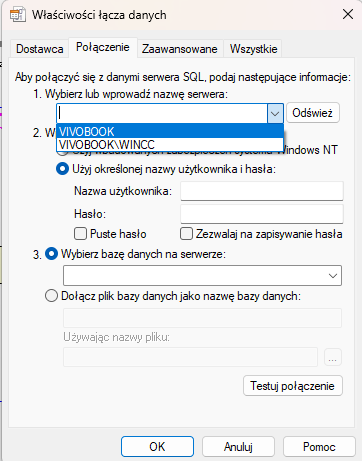
\includegraphics[width=0.6\textwidth]{src/Database/Stage3.png}
    \caption{Wybór nazwy serwera}
    \label{fig:first-att}
\end{figure}

\begin{figure}[H]
    \centering
    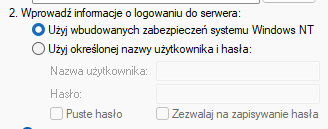
\includegraphics[width=0.6\textwidth]{src/Database/Stage4.png}
    \caption{Wporwadzenie informacji o logowaniu na serwer}
    \label{fig:first-att}
\end{figure}

\begin{figure}[H]
    \centering
    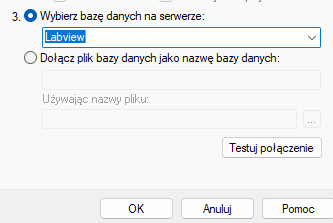
\includegraphics[width=0.6\textwidth]{src/Database/Stage5.png}
    \caption{Wybór odpowiedniej bazy danych z serwera}
    \label{fig:first-att}
\end{figure}

\begin{figure}[H]
    \centering
    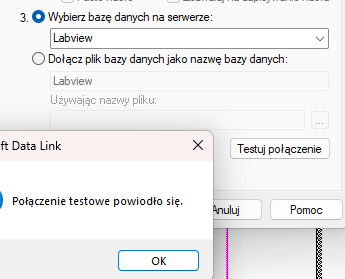
\includegraphics[width=0.6\textwidth]{src/Database/Stage6.png}
    \caption{Przetestowanie utworzonego połączenia}
    \label{fig:first-att}
\end{figure}

\begin{figure}[H]
    \centering
    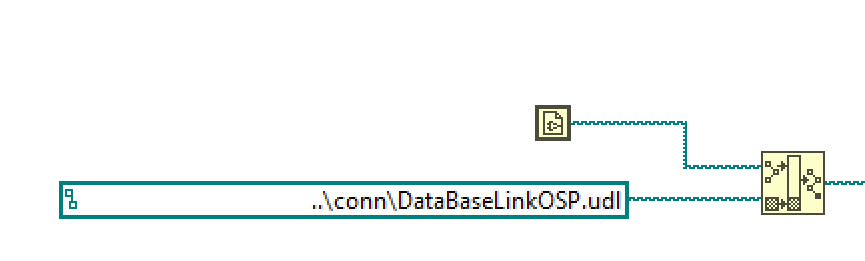
\includegraphics[width=0.6\textwidth]{src/Database/Stage7.png}
    \caption{Wprowadzenie ścieżki względnej do utworzonego linku .udl}
    \label{fig:first-att}
\end{figure}



\newpage
\subsubsection{\large Wykorzystanie SubVi DatabaseRead}

W celu poprawnego wyświetlenia informacji zwrotnej, kto aktualnie został zalogowany, konieczne było przygotowanie odpowodniej
SubVi. Jej zadaniem jest przechwycenie informacji zwrotnej uzyskanej przez skrypt w pythonie i porównanie jej z dostępnymi osobami w bazie. 

\begin{figure}[H]
    \centering
    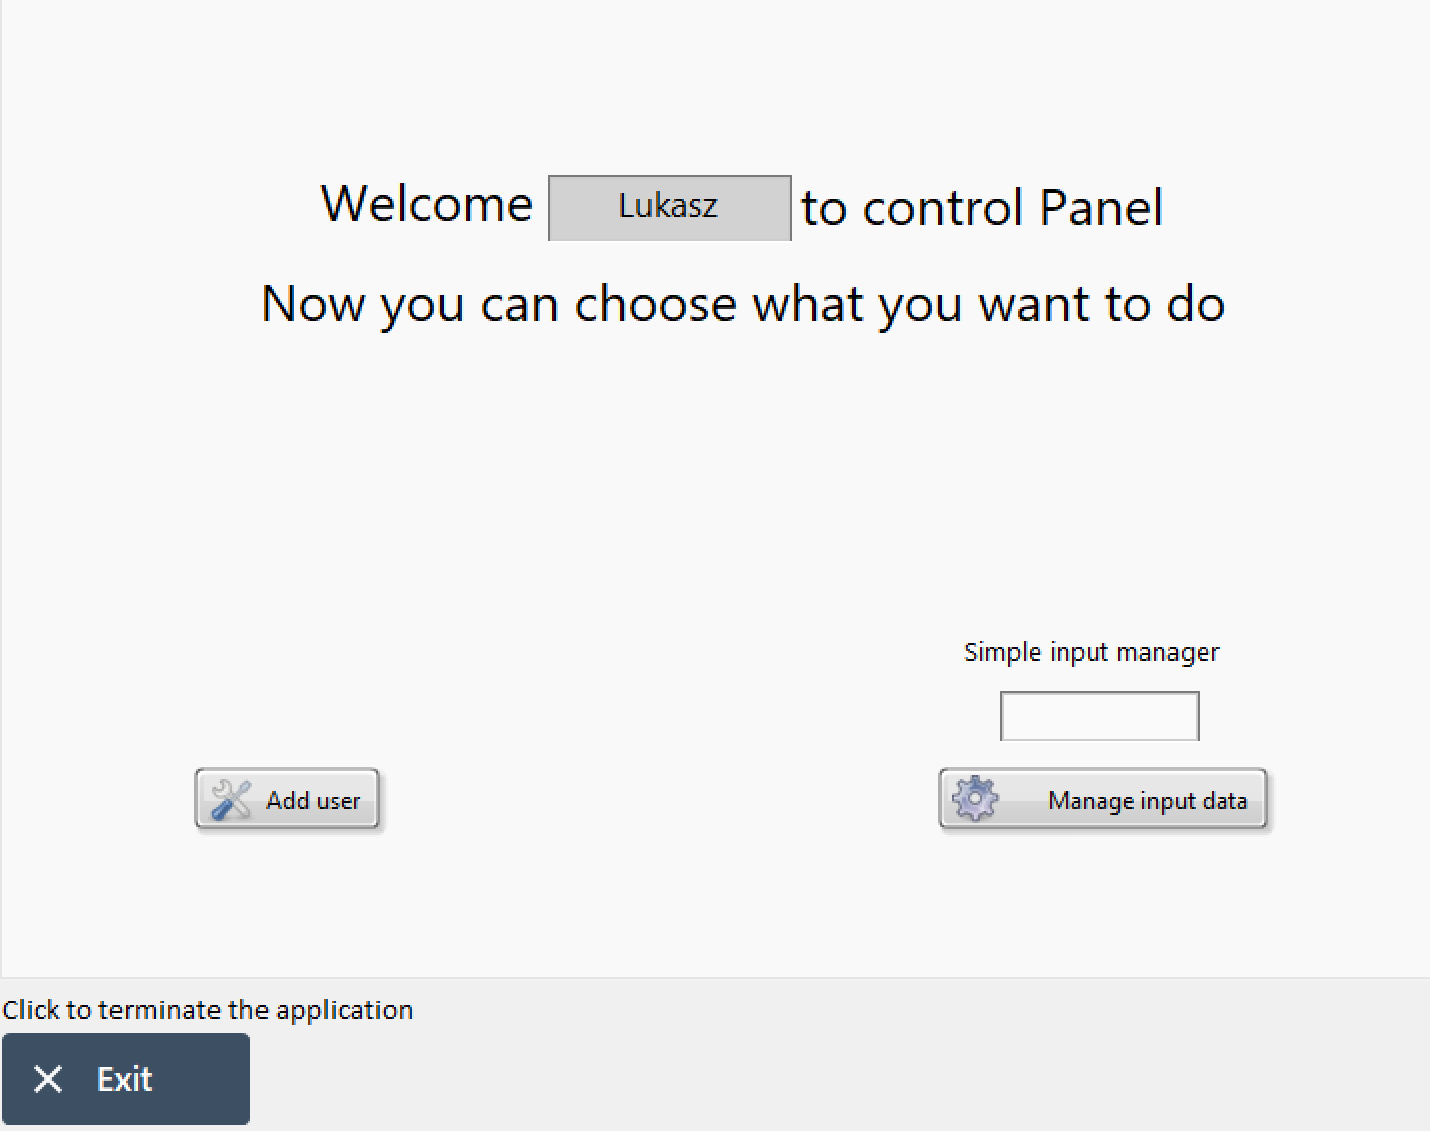
\includegraphics[width=0.7\textwidth]{src/Logged.png}
    \caption{Obraz przedstawiający główny widok aplikacji po zalogowaniu}
    \label{fig:first-att}
\end{figure}

Skrypt w pythonie został tak przekształcony, że w zależności od wyniku jeśli nie wykryto żadnej osoby to zwraca wartość zmiennej string "False".
Natomiast jeśli wykrył daną osobę, kóra znajduje się w pliku z obrazami referencyjnymi to zwraca nazwę obrazu wraz z rozszerzeniem, którego wynik był najbardziej zgodny.
Kolejno ścieżka do pliku przesyłana jest do bloku porównującego jak i przygotowanej SubVi.

\begin{figure}[H]
    \centering
    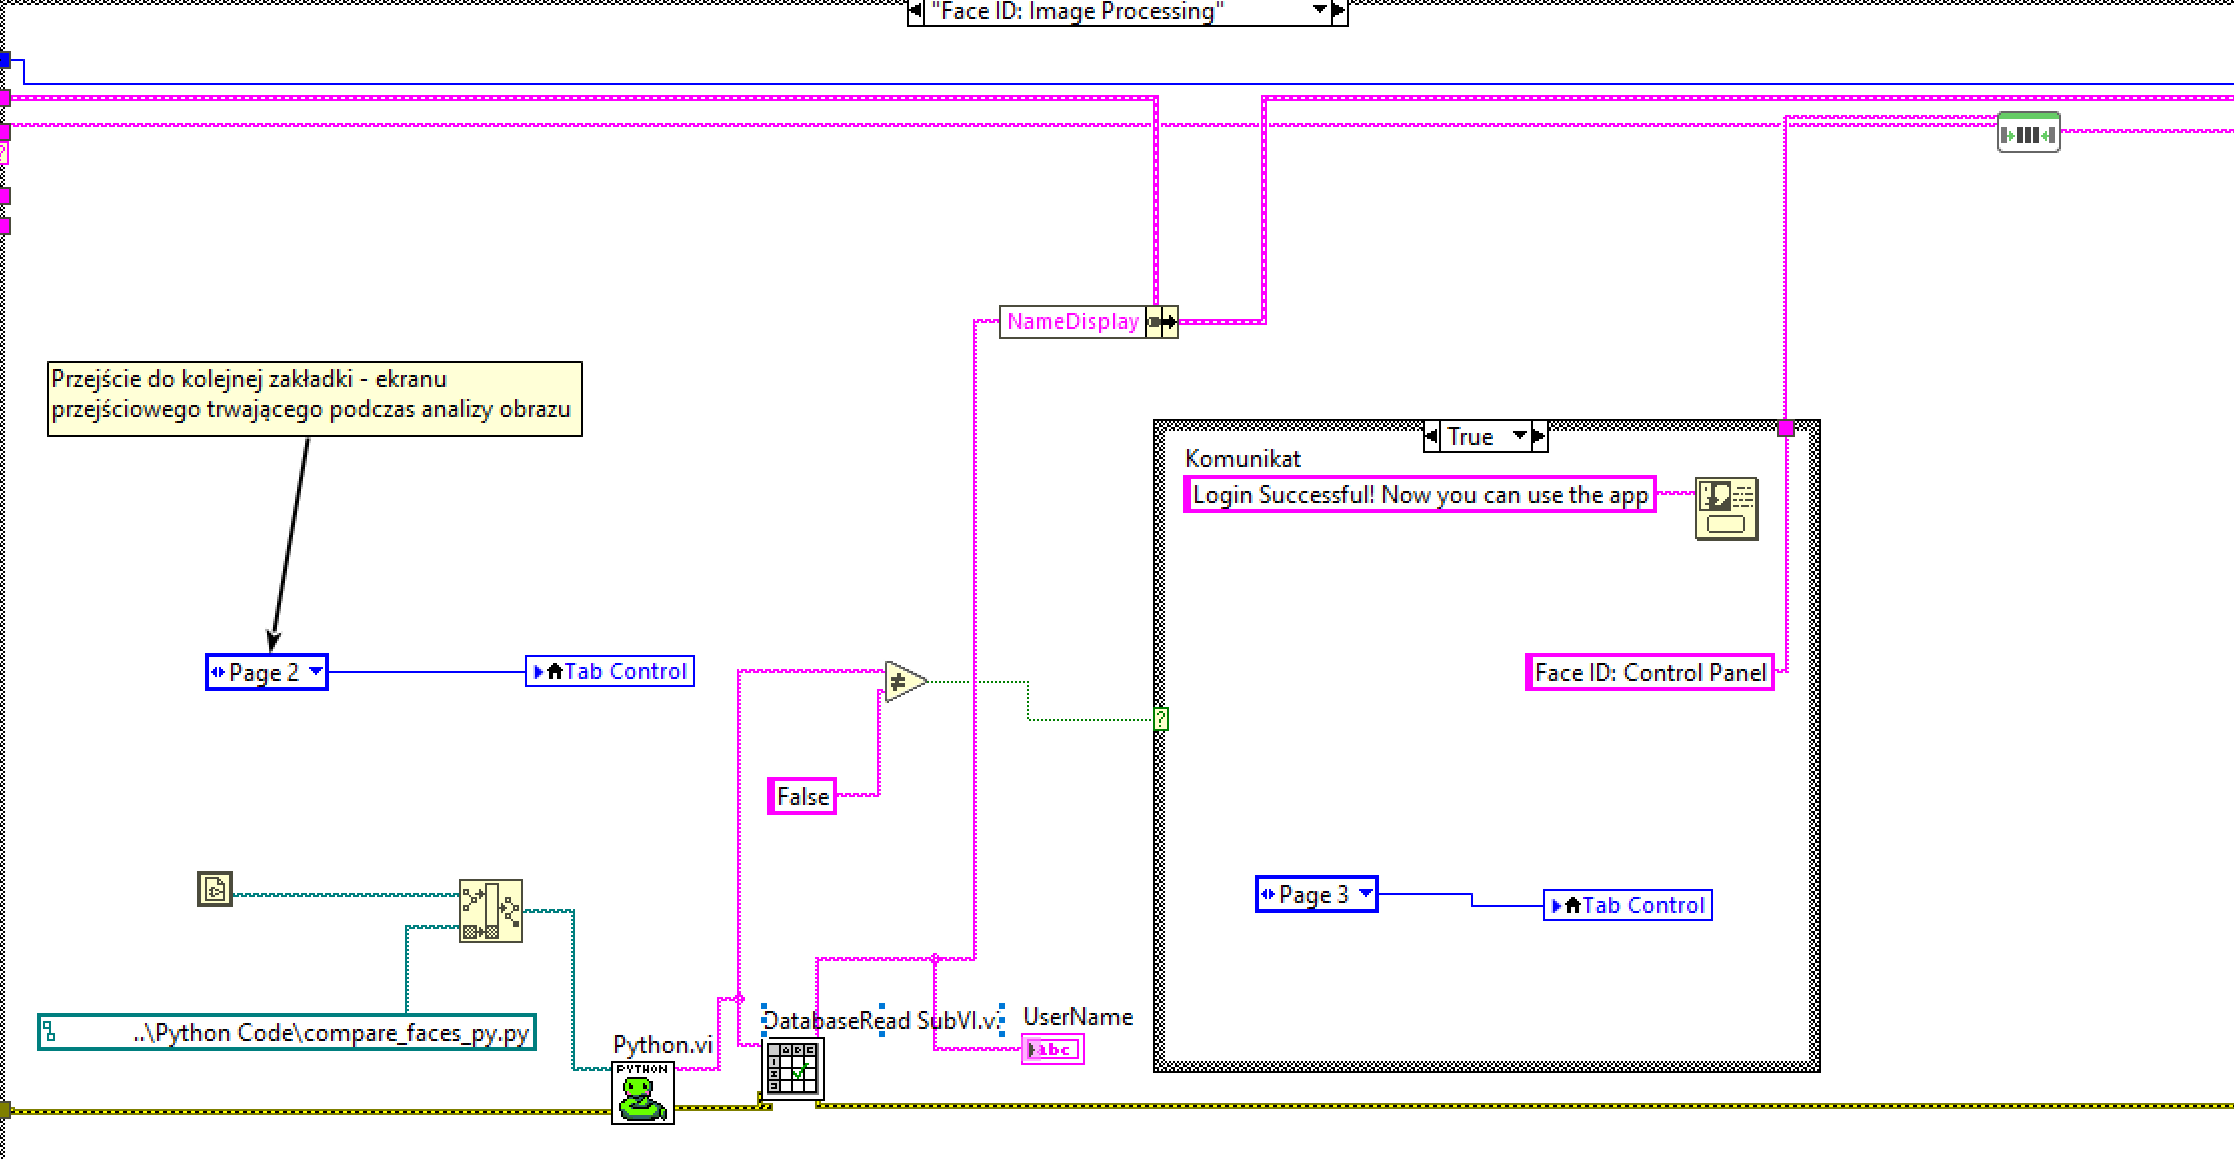
\includegraphics[width=0.9\textwidth]{src/Database/Database_read.png}
    \caption{Obraz przedstawiający implemenctację SubVi w maszynie stanów}
    \label{fig:first-att}
\end{figure}

Utworzona SubVi jako wejście przyjmuje string wzorcowowy zawierającego nazwę pliku (File name) oraz jako wyjście oddaje wynik czyli UserName.
Dodatkowo w celu kontroli nad pracą programu zostały dodane tablice: Porównanie (subarray) wyświetla ona nazwy wszystkich plików dostępnych w bazie oraz Data, która zwraca
całą zawartość bazy danych. Konieczne również było podłączenie z bazą poprzez wygenerowany link. Takowy link był wybierany w polu connection information, 
jednakże zostało to zastąpione przez ścieżkę względną.

\begin{figure}[H]
    \centering
    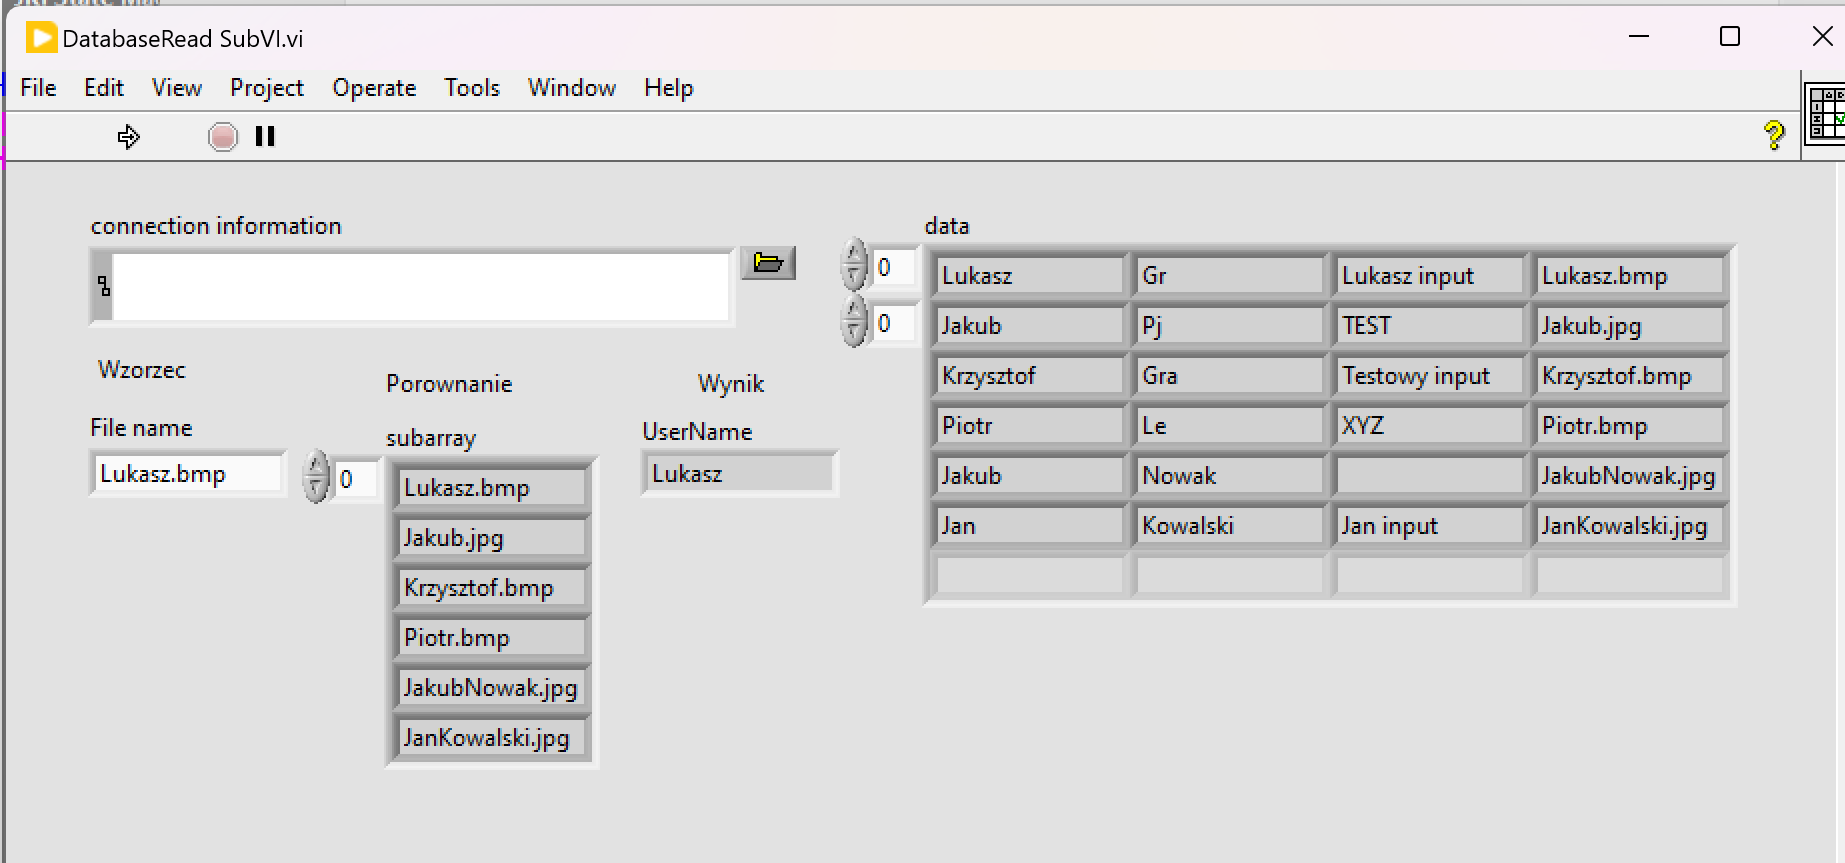
\includegraphics[width=1.0\textwidth]{src/Database/Database_read_subvi_frontpanel.png}
    \caption{Obraz przedstawiający Front Panel }
    \label{fig:first-att}
\end{figure}

Block Diagram składa się z prostych trzech bloków DB Tools potrzebnych do poprawnego odczytu informacji z bazy danych (Open Connection, Select Data, Close Connection).
Natomiast aby spełnić główne założenie SubVi niezbędne było dodanie funkcji sprawdzającej.
Elementy z bazy zostają odpowiednio wyselekcjonowane najpierw przez blok Database variant to data a następnie Index Array w celu wydobycia tylko jednej kolumny czyli Nazwa pliku.
Problem jednak pojawia się przy porównywaniu otrzymanej kolumny z wartością wzorcową File name otrzymaną z Pythona. Elementy w bazie danych oprócz nazwy plików zawierają znaki białe więc ich
usunięcie było konieczne do porównywania obydwu wyników. Dlatego więc wykorzystano funkcję for oraz blok trim whitespace. Funkcja iteruje po każdym wierszu z kolumny usuwając znaki białe.
Po takim zabiegu, porównywanie działa poprawnie i przy użyciu funkcji case zwracany jest UserName osoby dla której ścieżka do pliku okazała się być zgodna z tym co zwrócił skrypt w Pythonie a
wynik jest wyświetlany na ekranie głównym aplikacji.

\begin{figure}[H]
    \centering
    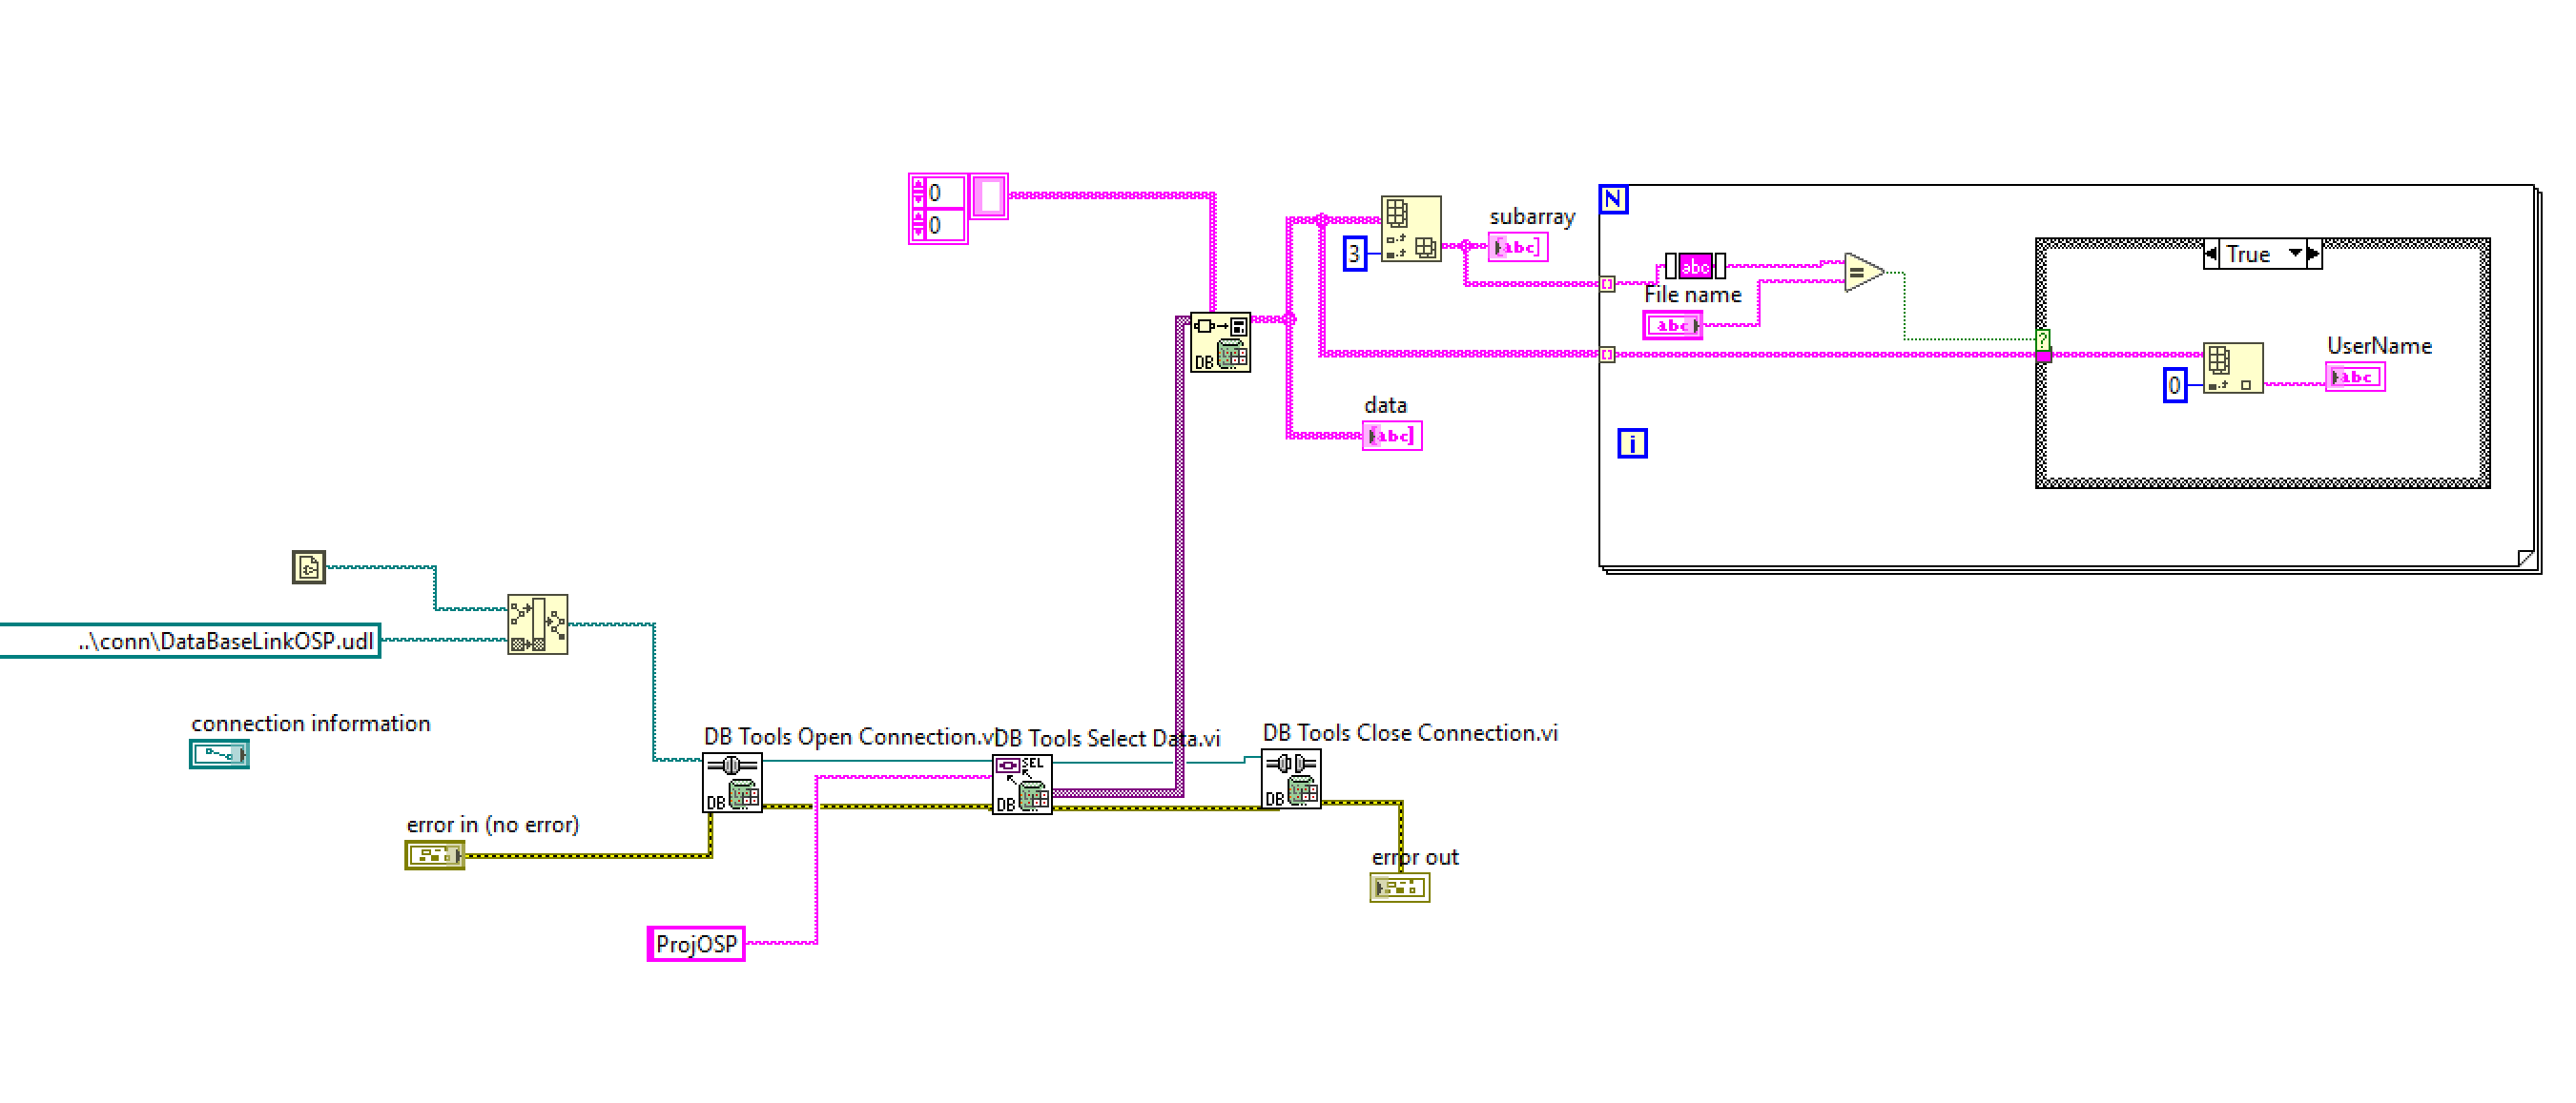
\includegraphics[width=1.0\textwidth]{src/Database/Database_read_subvi.png}
    \caption{Obraz przedstawiający Block Diagram }
    \label{fig:first-att}
\end{figure}

\subsubsection{\large Wykorzystanie SubVi DatabaseWrite}

Implementacja SubVi DatabaseWrite jest stosunkowo najłatwiejsza w porównaniu do reszty SubVi. Specjalnie do tego celu został zmodyfikowany stan Add User: Grab Input Image.
Przygotowana SubVi, tak jak stan, ma na celu dodanie nowego użytkownika a do pliku zostaje zapisane zdjęcie, które będzie wzorcem dla programu, jego nazwa to imie (Name) i Nazwisko (Surname) w formacie .jpg
wpisane przez użytkownika. Natomiast do bazy przesyłane są takie informacje jak imię, nazwisko oraz nazwa pliku, który został zapisany w odpowiednim rozszerzeniu.
Dodatkowo w celu uniknięcia zawieszenia aplikacji zastosowano rozwiązanie polegające na przesłaniu odpowiedniego stanu w kolejce. 

\begin{figure}[H]
    \centering
    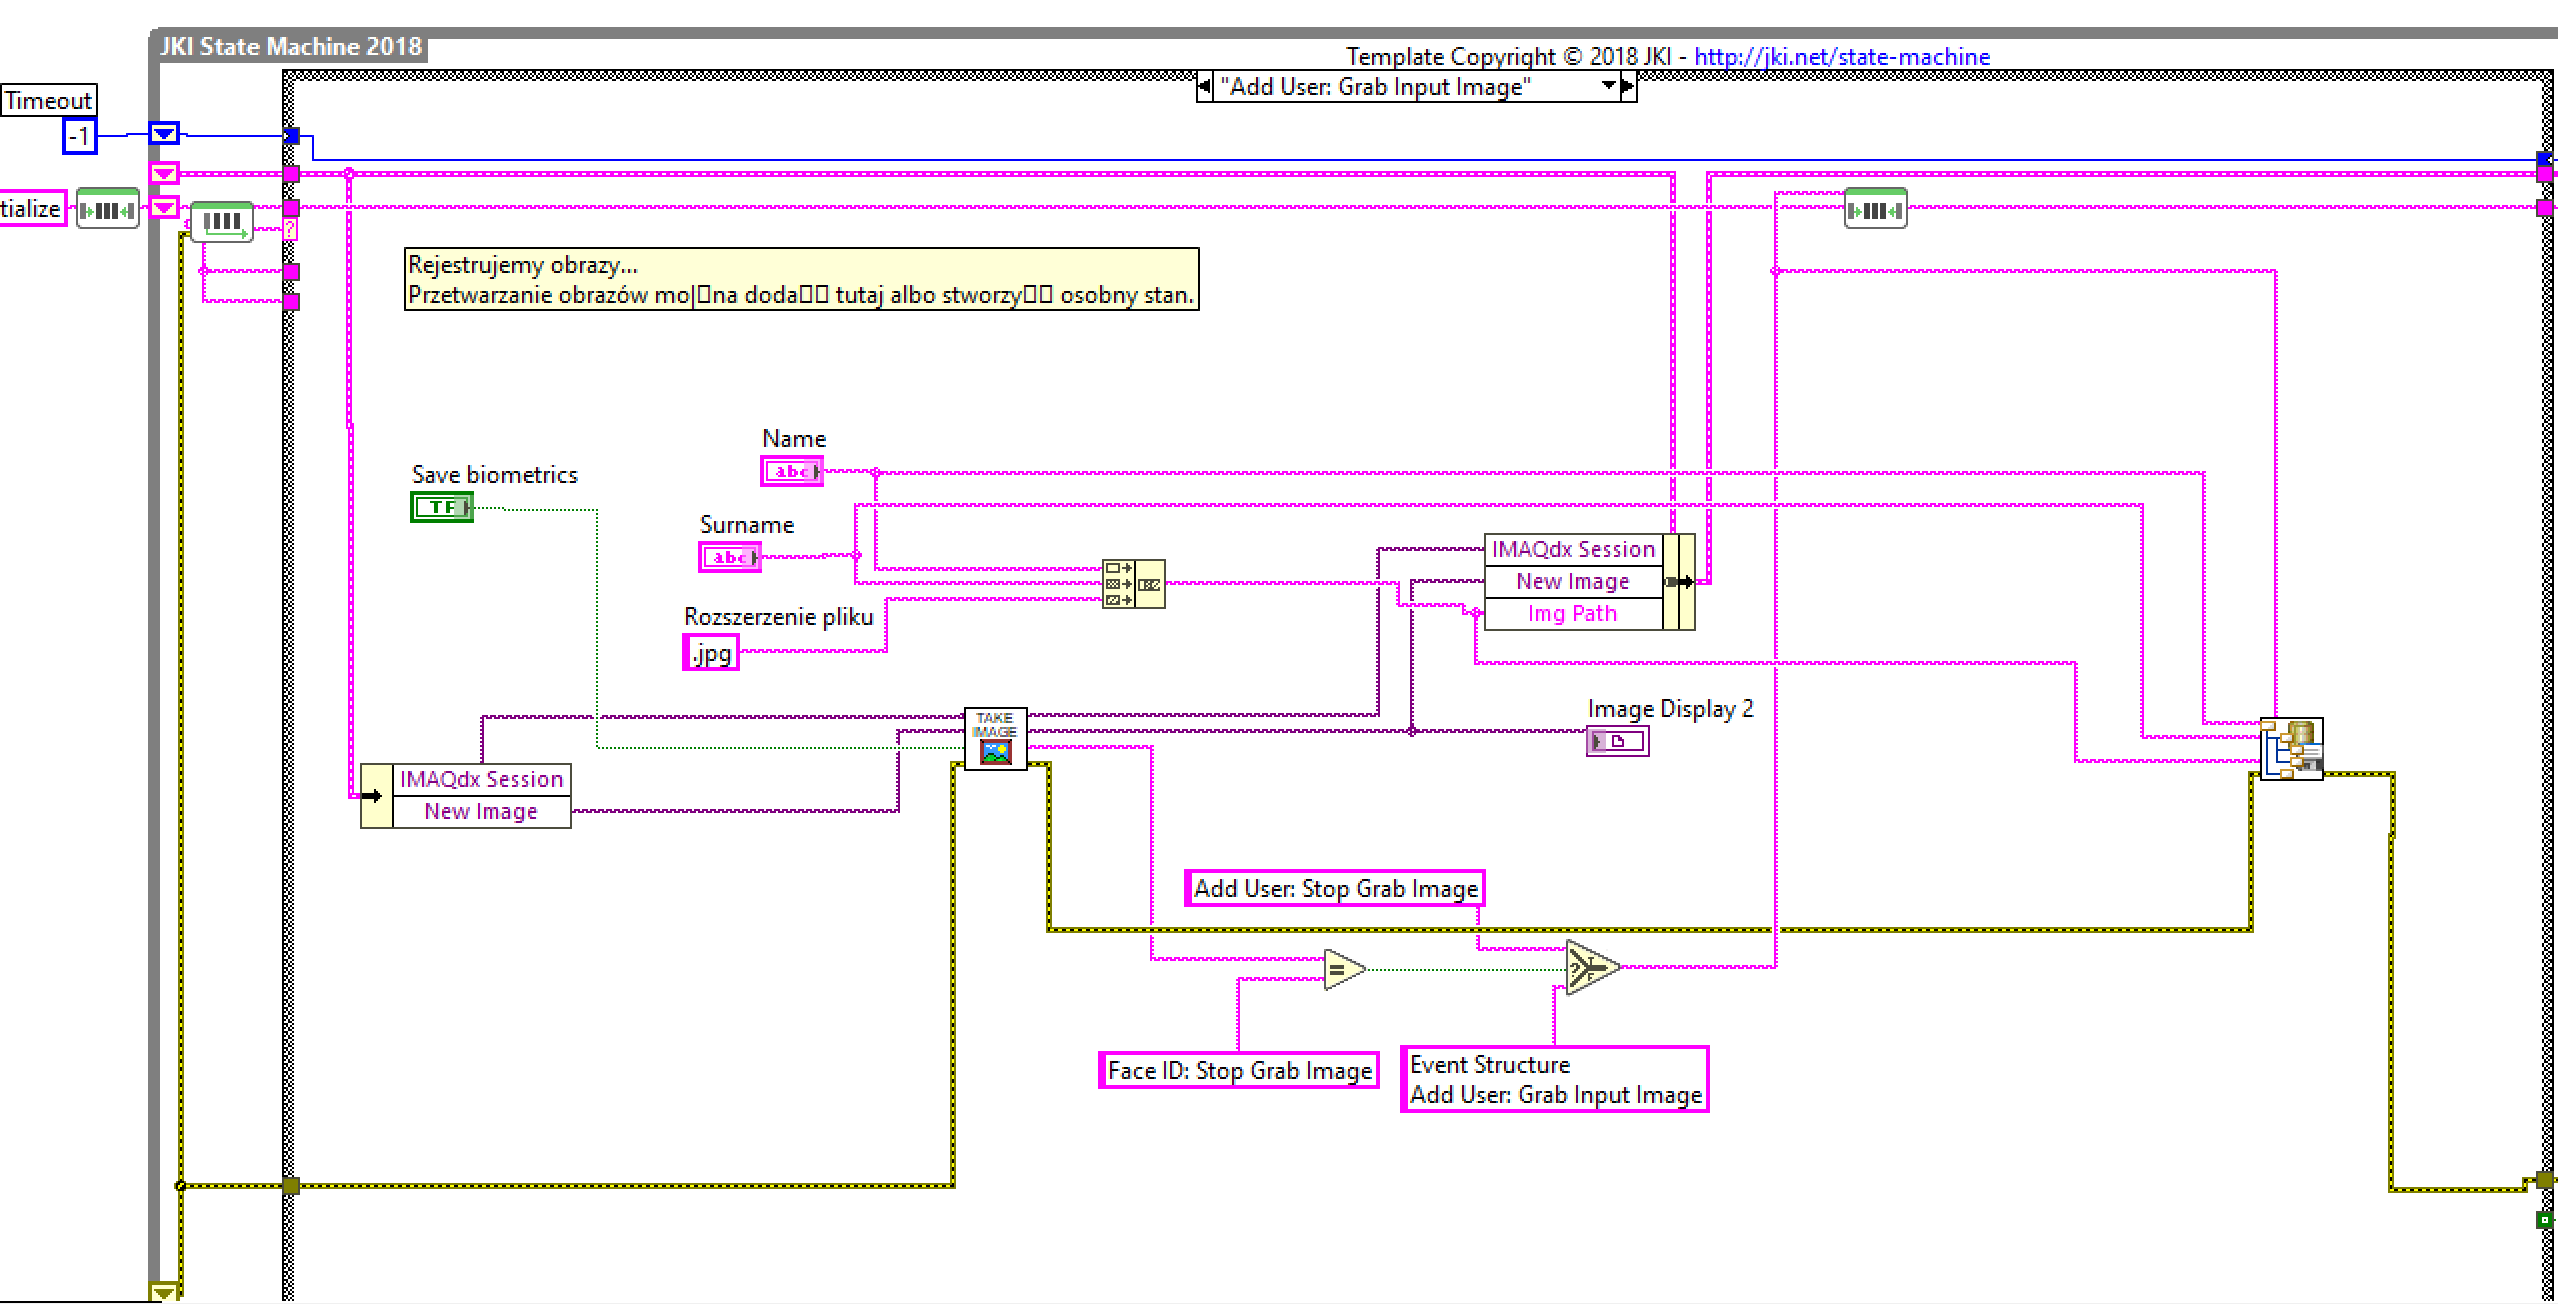
\includegraphics[width=0.9\textwidth]{src/Database/Database_write.png}
    \caption{Obraz przedstawiający implemenctację SubVi w maszynie stanów}
    \label{fig:first-att}
\end{figure}

\begin{figure}[H]
    \centering
    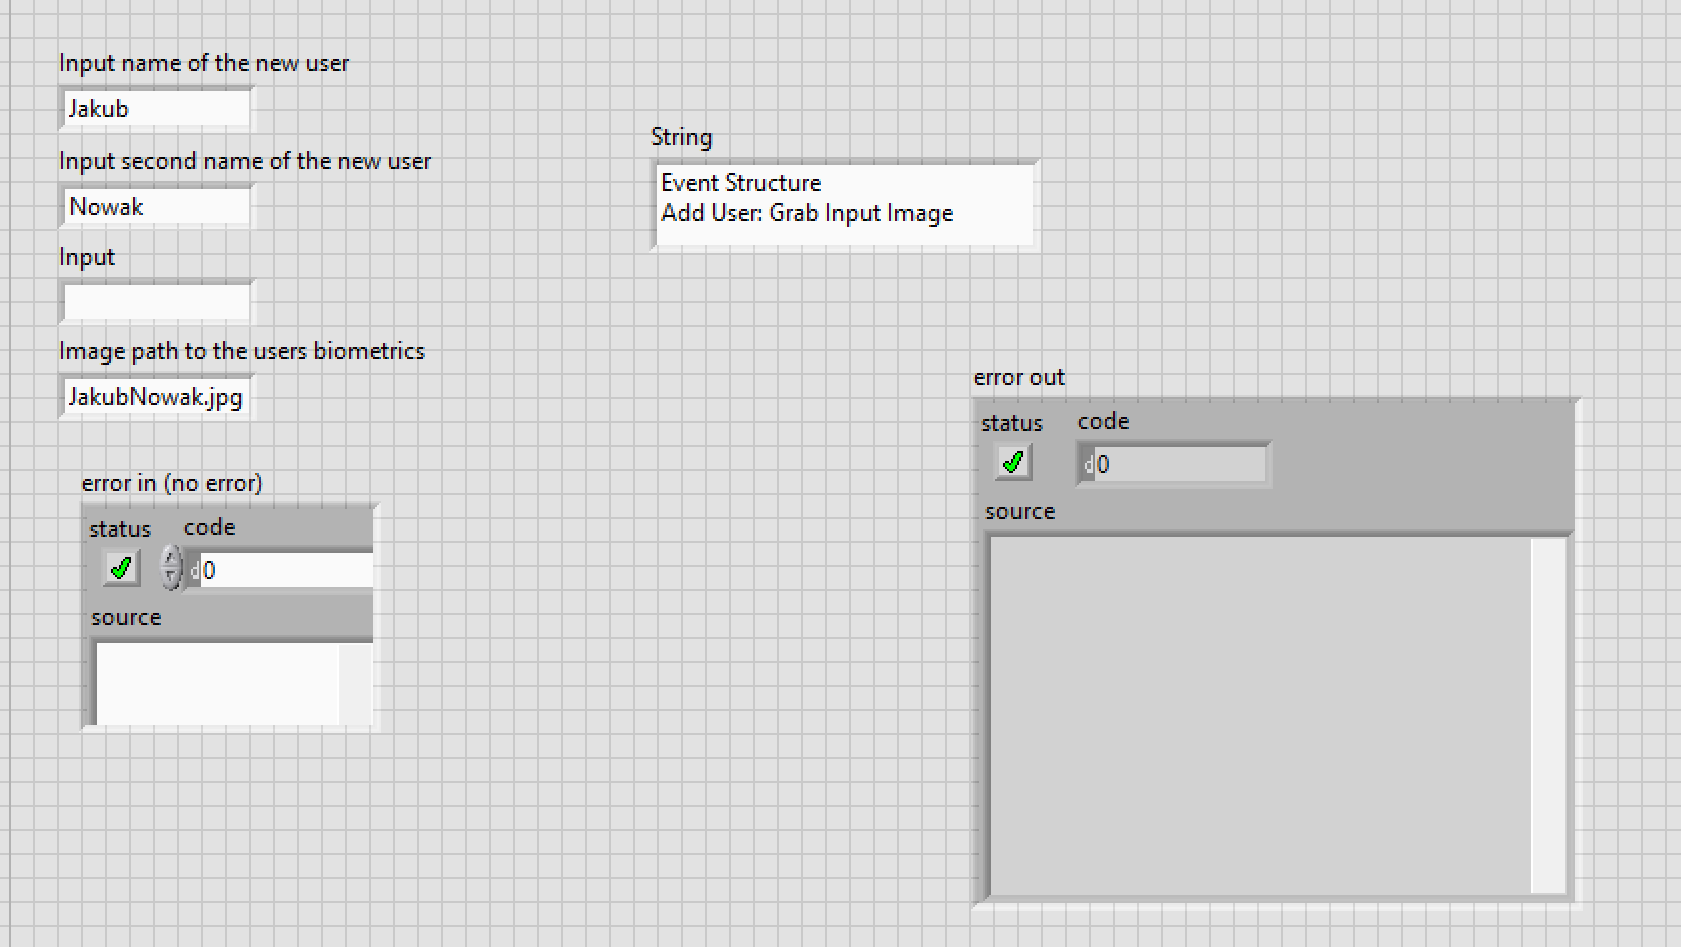
\includegraphics[width=0.9\textwidth]{src/Database/Database_write_subvi_frontpanel.png}
    \caption{Obraz przedstawiający Front Panel}
    \label{fig:first-att}
\end{figure}

Przygotowana struktura case w Block Diagram ma na celu zapobieganie zawieszanie się programu. Przy takim rozwiązaniu wpisanie danych do bazy
nastąpi tylko wtedy gdy zostanie wciśnięty przycisk Save biometrics. W momencie, gdy nie było struktury case, nowy użytkownik był wpisywany ciągle, niezależnie od stanu przycisku
a program zawieszał się.
Funkcja składa się z trzech bloków DB Tools (Open Connection, Insert Data, Close Connection). W miejscu insert data przyjmowana jest nazwa tabeli, nazwy kolumn oraz wartości jakie mają zostać dodane.

\begin{figure}[H]
    \centering
    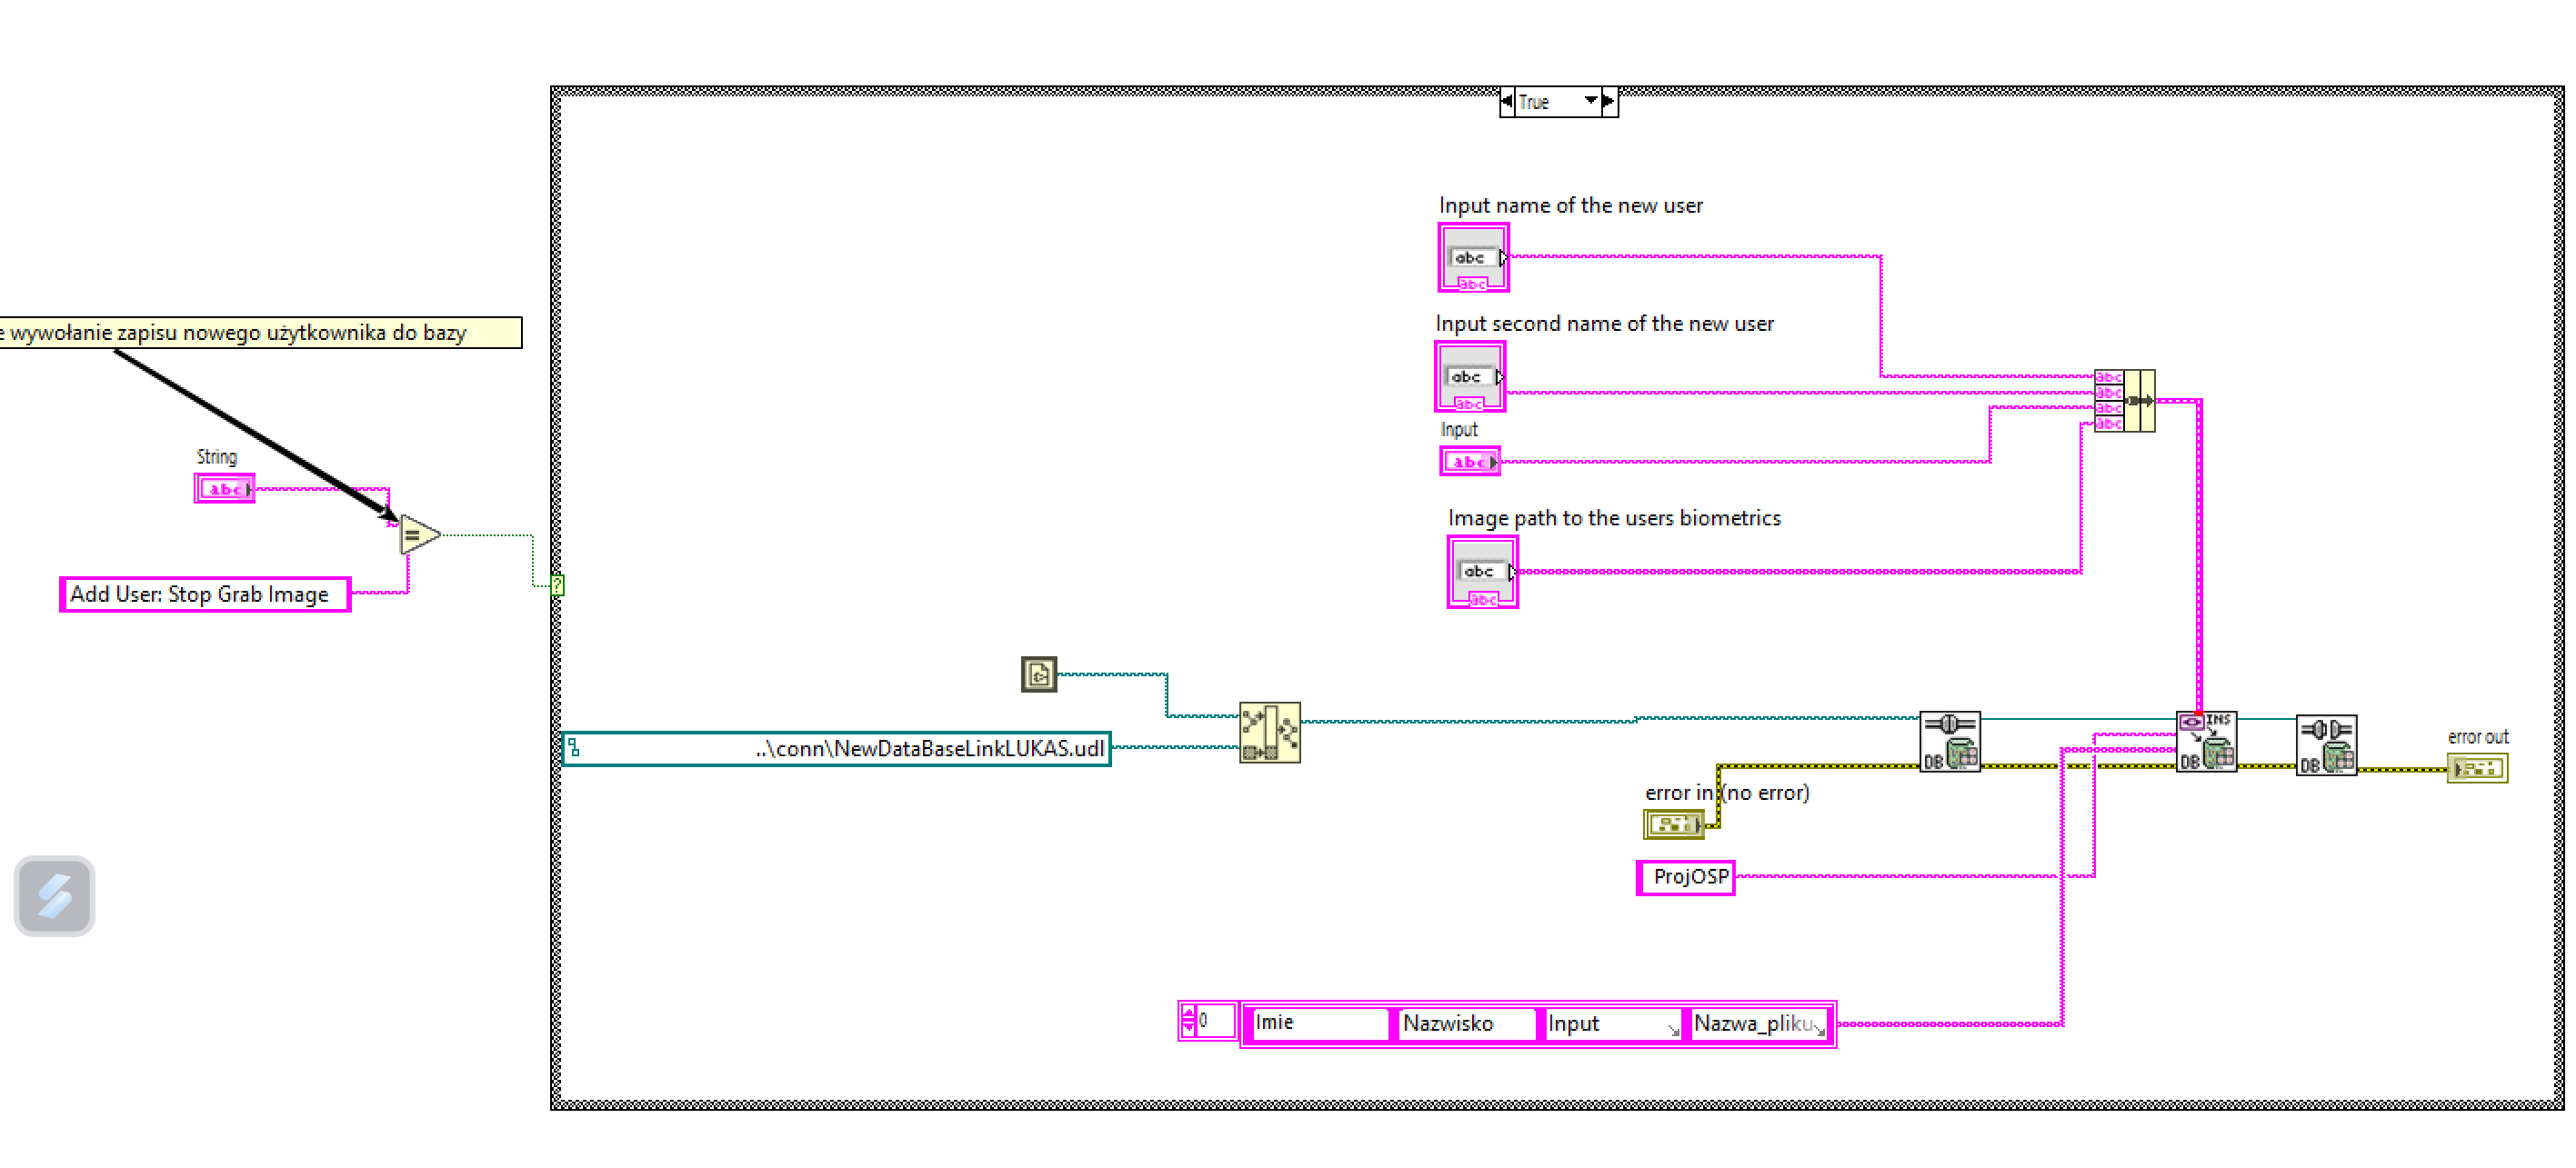
\includegraphics[width=0.9\textwidth]{src/Database/Database_write_subvi.png}
    \caption{Obraz przedstawiający Block Diagram}
    \label{fig:first-att}
\end{figure}

\subsubsection{\large Wykorzystanie SubVi DatabaseUpdate}

Wykorzystanie SubVi DatabaseUpdate stanowiło największe wyzwanie ze względu na swoją złożoność i logikę w Block Diagram. Zmodyfikowano Face ID: Control Panel o nowy Event
Manage input data: Value change. SubVi read przyjmuje jako wejście dwie wartości: NameDisplay czyli imie jakie jest aktualnie wyświetlane na ekranie głównym oraz pole input, które 
służy do prostej obsługi danych w aplikacji.

\begin{figure}[H]
    \centering
    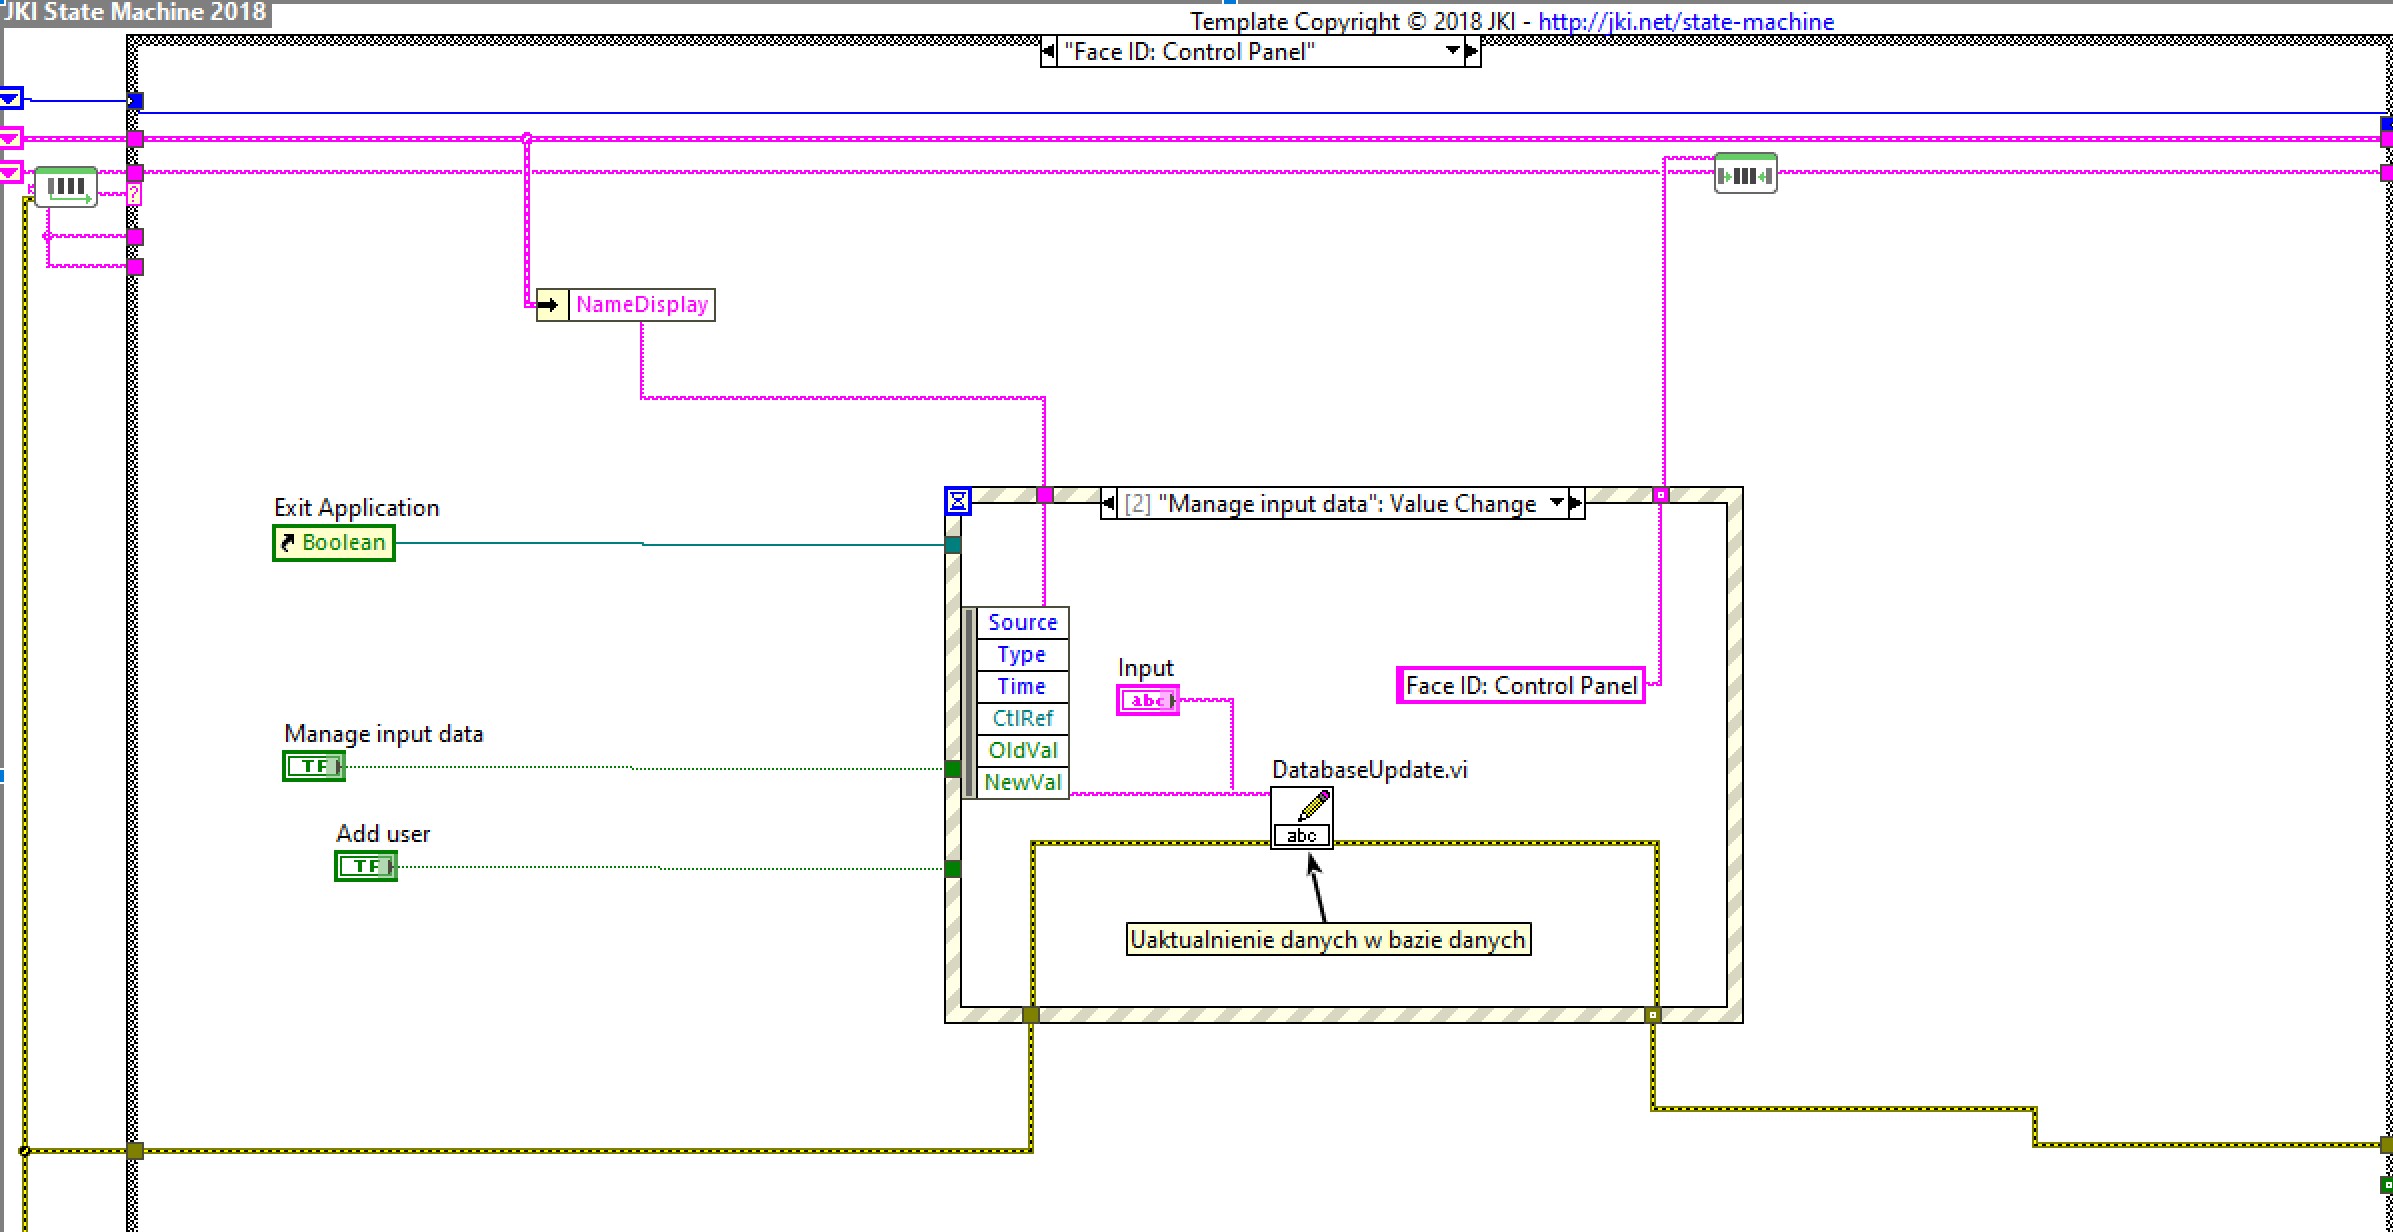
\includegraphics[width=0.9\textwidth]{src/Database/Database_update.png}
    \caption{Obraz przedstawiający implemenctację SubVi w maszynie stanów}
    \label{fig:first-att}
\end{figure}

Front panel zawiera takie elementy jak Imie czyli dana jaka jest przekazywana po zalogowaniu przez użytkownika, Input czyli pole na wpisanie dowolnej formuły indywidualnie przez użytkownika,
Numer wiersza jest on konieczny do poprawnego zlokalizowania komórki przez program, Final Data czyli tablica pokazująca tablicę bazy danych po zmianach oraz Initial Data czyli tablica pokazująca
dane przed zmianą.

\begin{figure}[H]
    \centering
    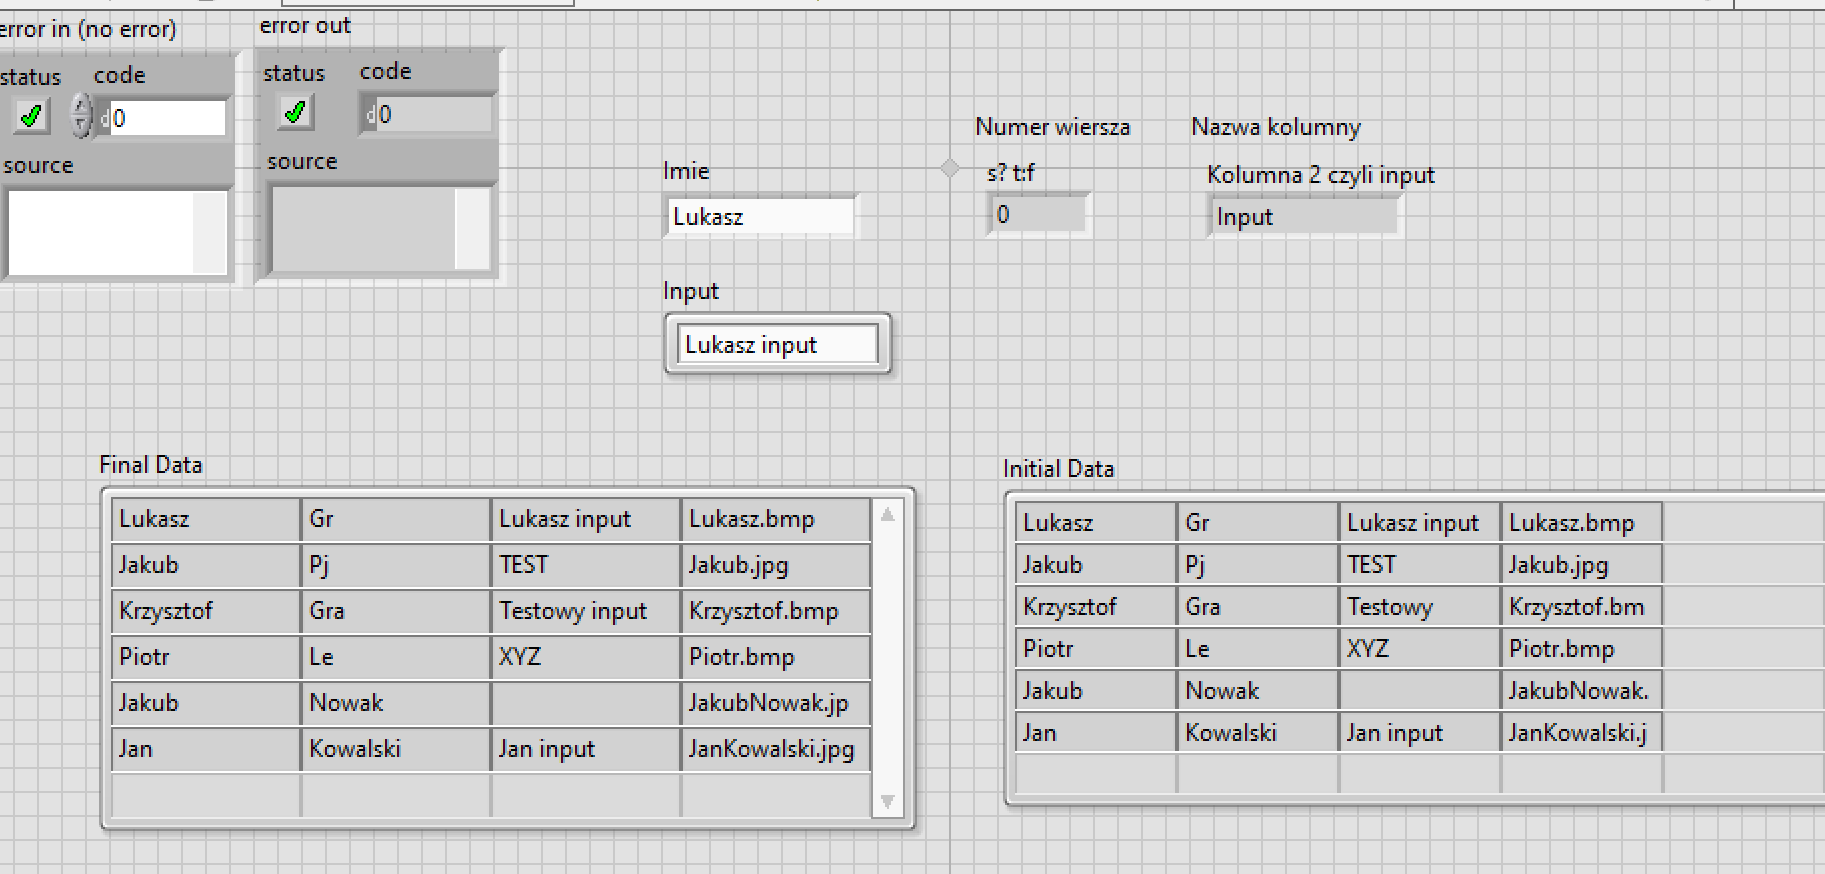
\includegraphics[width=0.9\textwidth]{src/Database/Database_update_subvi_frontpanel.png}
    \caption{Obraz przedstawiający Front Panel}
    \label{fig:first-att}
\end{figure}

Przedstawiona SubVi jest zmodyfikowaną wersją dostarczonego przez producenta przykładu do użycia bloku DB Tools Update Data. Składa się ona z wielu elementów lecz główna logika dzieje się w górnej części.
Tak jak w przypadku poprzednich SubVi, dane z bazy są pobierane przez bloki (Open Connection, Select Data, Varian To Data, Tools List Columns), aby móc porównać elementy z komórek konieczne było wykorzystanie
funkcji for do iterowania przez każdy element tablicy tak jak w przypadku SubVi DataBaseRead. Gdy program wykrył zgodność wyświetlanego imienia wraz z elementem w bazie, dalej przesyłany zostaje numer iteracji,
który będzie jednocześnie numerem wiersza (indeksu) w bazie. Ten numer przekazywany jest do bloków Index Array i dzięki ich pomocy, jest możliwa zmiana wartości bloku input dla konkretnego użytkownika.
Aby wszystko mogło poprawnie działać, konieczne jest jeszcze wykorzystanie polecenia SQL mającego na celu zamienienie wartości w komórkach kolumny input.
Dodatkowo cały proces przed i po wyświetlany jest podwójne użycie funkcji for na początku i końcu programu.

\begin{figure}[H]
    \centering
    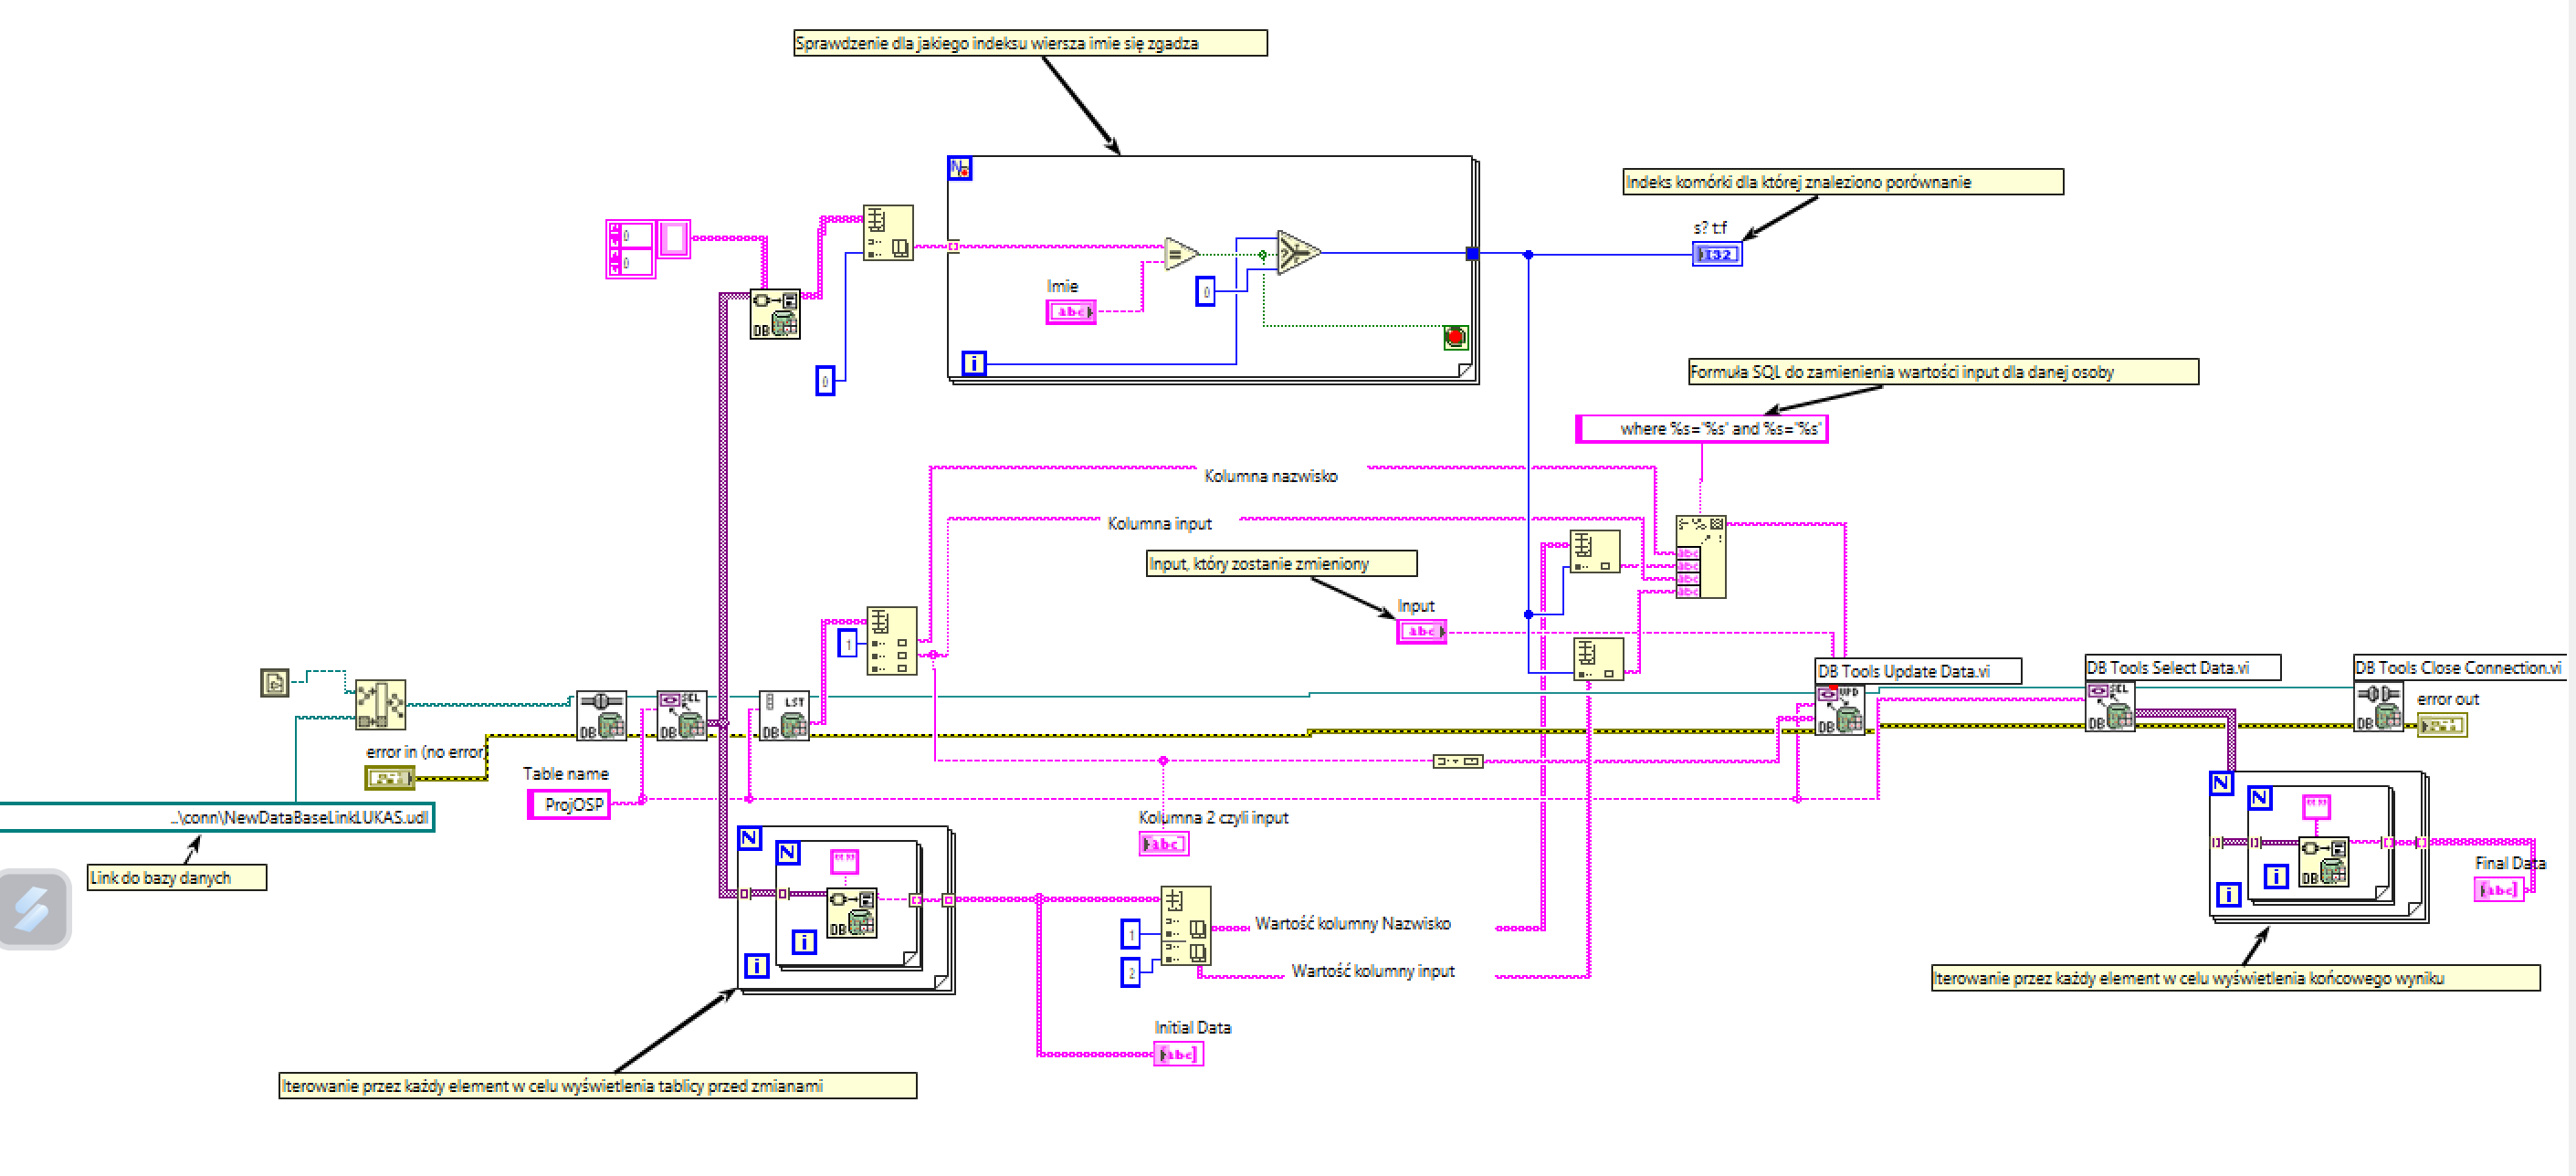
\includegraphics[width=1.0\textwidth]{src/Database/Database_update_subvi.png}
    \caption{Obraz przedstawiający Block Diagram}
    \label{fig:first-att}
\end{figure}

\newpage
\subsection{\Large Instrukcja korzystania z aplikacji}

W aplikacji zostały umieszczone podpowiedzi, dotyczące m.in. ustawienia się do kamery oraz informacje do czego służą przyciski. Jednakże wartym dodania jest instrukcji
jak powinno się korzystać za aplikacji aby po przy pierwszym uruchumieniu działała poprawnie. 

Przed uruchomieniem aplikacji głównej należy uruchomić SubVi oznaczoną nazwą DatabaseRead SubVi. Aplikacja powinna wtedy zaczerpnąć informacje z bazy, jeśli tego nie zrobiła
kluczowe będzie wygenerowanie linku połączenia do bazy zgodnie z podrozdziałem 2.7.1. Kluczowe jest aby tabela bazy danych posiadała kolumny Imie, Nazwisko, Input oraz Nazwa Pliku.

\begin{figure}[H]
    \centering
    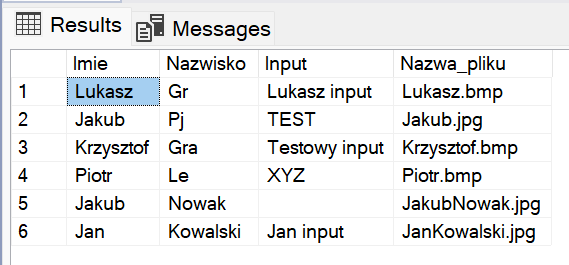
\includegraphics[width=0.6\textwidth]{src/Database/Microsoft SQL.png}
    \caption{Obraz przedstawiający przykładową tabelę}
    \label{fig:first-att}
\end{figure}

Gdy elementy z bazy danych zostaną zaczerpnięte aplikacja powinna działać sprawnie jednakże, jeśli korzysta z niej osoba, która nie jest zarejestrowana, nie uzyska ona bowiem dostępu.
W tym przypadku konieczne będzie dodanie wyraźnego zdjęcia przedstawiającego twarz użytkownika do folderu aplikacji Data -> Registered Users. Po tym zabiegu aplikacja powinna wpuścić nowego użytkownika
i będzie możliwe dodanie go do bazy danych poprzez wciśnięcie przycisku Add User i nadaniu Imienia i Nazwiska. Aplikacja wykona wtedy nowe zdjęcie z nazwą pliku odpowiadającemu podanemu Imieniu oraz Nazwisku.
Po tym zabiegu będzie można usunąć stare (tymczasowe) zdjęcie z folderu Registered Users



\section{\LARGE Napotkane problemy}
\subsection{\Large Implementacja zakładek}

Ze względu na charakter aplikacji wymagane jest użycie zakładek, implementacja czego nie była oczywista w środowisku LabView. Kluczowym elementem używania zakładek lub też tzw. Tabs, jest użycie bloku \textit{Tab Control}. Jednakże, ze względu na ograniczoną ilość dostępnych materiałów na ten temat w internecie wdrożenie tego rozwiązania okazało się dużym wyzwaniem. 

Pierwsza wersja aplikacji zawierała wszystkie zakładki w jednym stanie - \textit{UI: Initialize}. Jak nietrudno się domyślić, rozwiązanie to było z zasady błędne, ponieważ nie wykorzystywało korzyści jakie daje framework JKI. 

\begin{figure}[H]
    \centering
    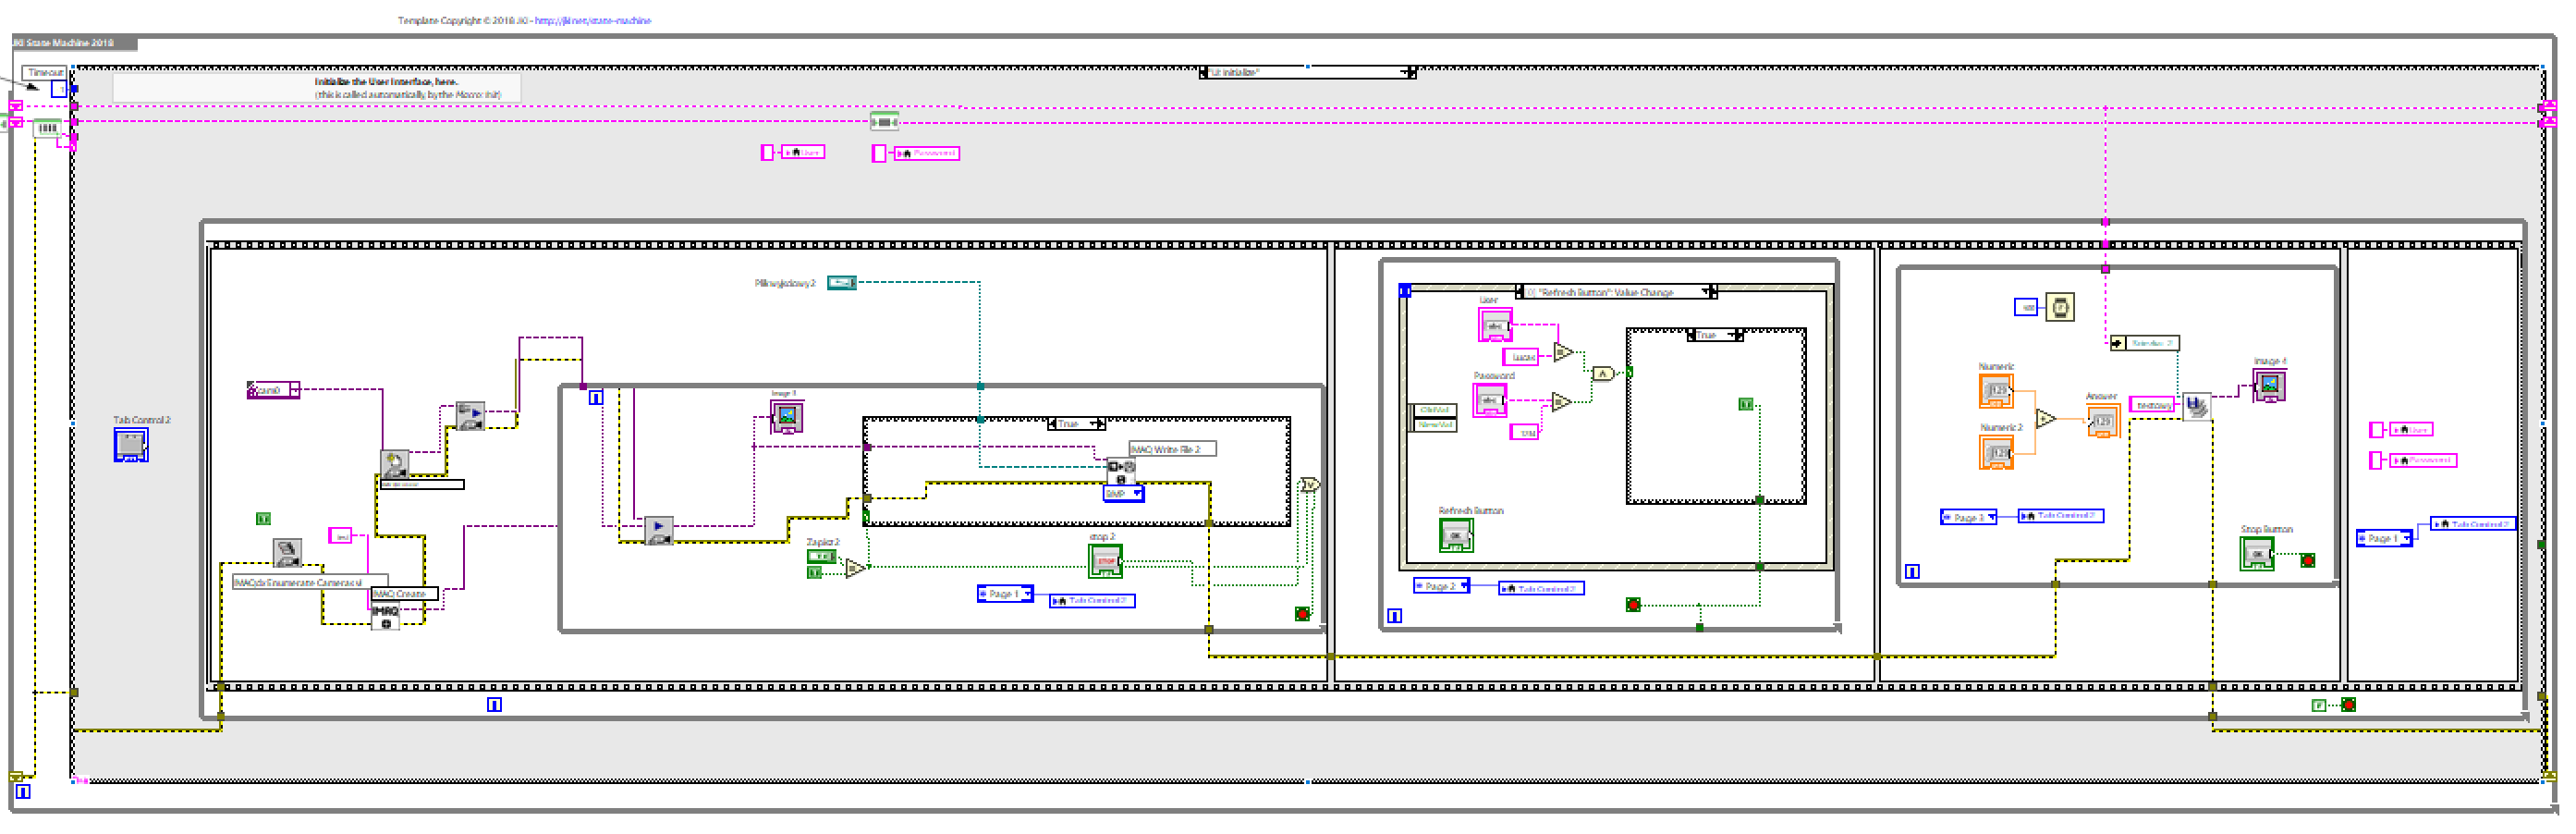
\includegraphics[width=1.0\textwidth]{src/first-att.png}
    \caption{Obraz przedstawiający pierwszą próbę implementacji struktury Tab Control}
    \label{fig:first-att}
\end{figure}

Następna próba rozwiązania również wykorzystywała strukturę \textit{Tab Control}, jednak tym razem implementacja była porawna, a więc wszystkie funkcjonalności podszczególnych zakładek zostały wyodrębnione do odpowiendnich stanów. 

Implementacja takiego rozwiązania jest możliwa poprzez dodanie globalnego bloku \textit{Tab Control}, znajdującego się na większości załączonych orbazów w prawym górnym rogu. Znaczenie słowa \textit{"globalnego"} oznacza w tym przypadku umieszczenie go poza strukturą \texttt{While}, rdzenia framework'a JKI.

Odpowiada on za obsługę oraz wyświetlenie całej struktury na interfejsie użytkownika. Przełączanie pomiędzy kolejnymi zakładkami jest realizowane również poprzez blok \textit{Tab Control} oraz dodanie do niego typu wyliczeniowego zawierającego nazwę strony, którą należy wyświeltić. 

\begin{figure}[H]
    \centering
    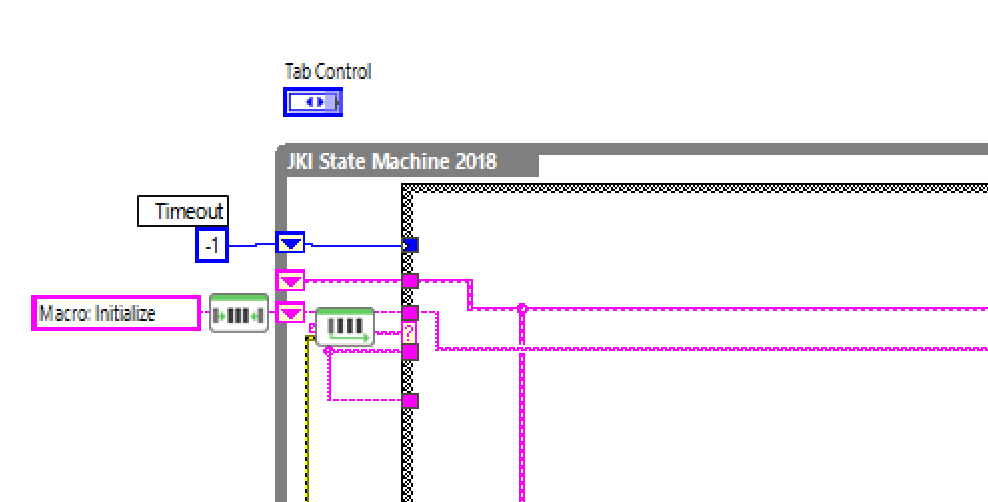
\includegraphics[width=0.5\textwidth]{src/tab-control.png}
    \caption{Obraz przedstawiający użycie bloku globalnego Tab Control}
    \label{fig:tab-control}
\end{figure}

\begin{figure}[H]
    \centering
    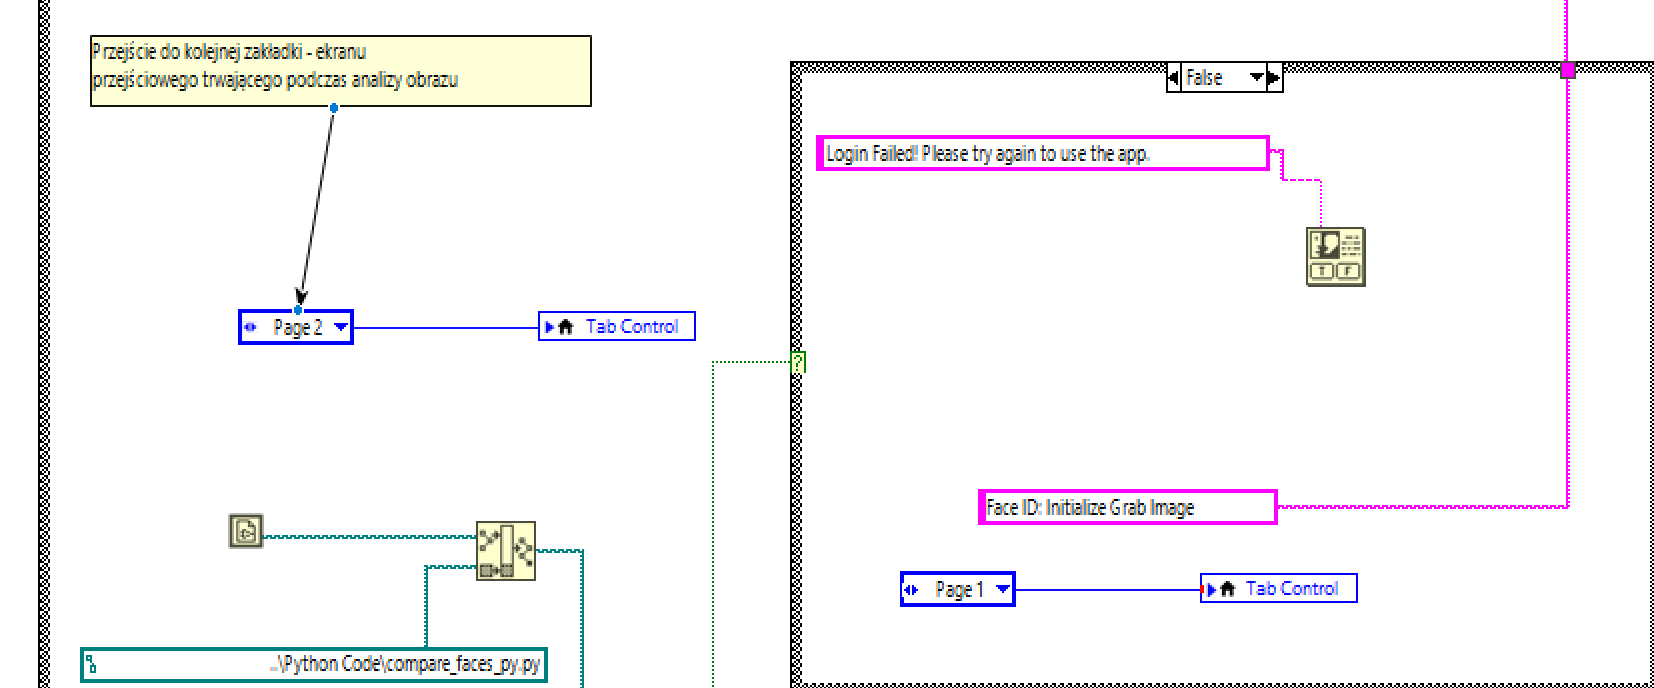
\includegraphics[width=0.5\textwidth]{src/tab-control-page.png}
    \caption{Obraz przedstawiający implementację przełączania między zakładkami}
    \label{fig:tab-control-page}
\end{figure}



\subsection{\Large Wywoływanie skryptów Python z poziomu LabVIEW}

% --------------------------------------------------------
% Autor: Krzysztof Grądek, Piotr Legień
%
% TODO: Opisać problemy napotkane podczas prób wywołania skryptów LabView z poziomu LabView
%
% Status: 100%
% --------------------------------------------------------
Pierwszym wyzwaniem było wybranie odpowiedniej wersji Pythona, kompatybilnej z używaną wersją LabVIEW. Sprawdzono która wersja najlepiej odpowiada wymaganiom i jest kompatybilna z face recognition i OpenCV. Po kilku próbach i testach wybrano wersję, która działała bezproblemowo z LabVIEW.

Kolejnym problemem było dostosowanie kodu Pythona do wymagań LabVIEW. Kod musiał zostać przebudowany, aby funkcje były jasno zdefiniowane za pomocą „def”, co umożliwiło ich wywoływanie z poziomu LabVIEW. Wprowadzono odpowiednie modyfikacje i przetestowano nowe funkcje, aby upewnić się, że działają poprawnie w środowisku LabVIEW.

Ostatnim wyzwaniem było podłączenie odpowiednich bloków w LabVIEW i stworzenie subVI, które realizowałoby całą operację wykonania skryptu Pythona.  Po kilku iteracjach i testach stworzono subVI, które działało poprawnie, umożliwiając płynne wykonywanie operacji Pythona z poziomu LabVIEW.
\begin{figure}[H]
    \centering
    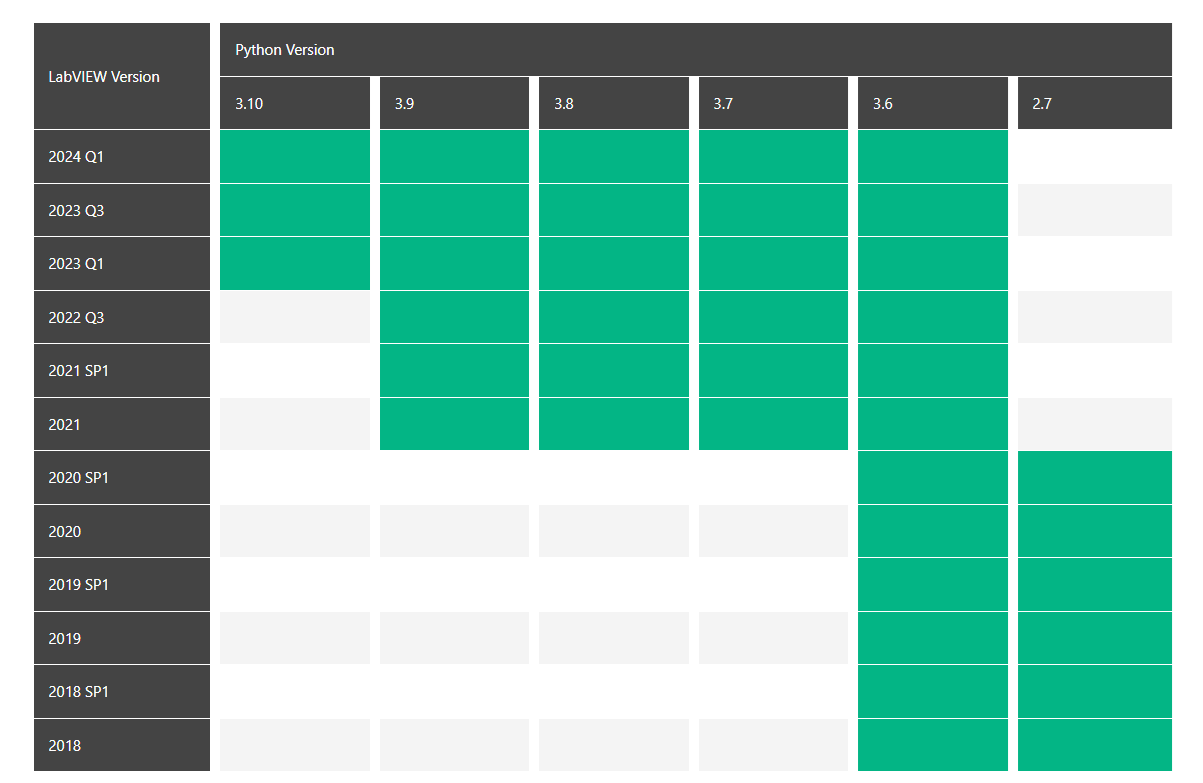
\includegraphics[width=0.6\textwidth]{src/python-v.png}
    \caption{Kompatybilność wersji pythona z wersjami Labview}
    \label{fig:python-version}
\end{figure}

\subsection{\Large Wykonanie działającego połączenia aplikacji z bazą danych SQL}

% --------------------------------------------------------
% Autor: Łukasz Grabarski
%
% TODO: Opisać problemy napotkane podczas prób połączenia LabView z bazą danych SQL Server
%
% Status: 100%
% --------------------------------------------------------

Głównym problemem przy połączeniu z bazą danych była manipulacja oraz porównywanie komórek w tablicy z wartościami dostarczanymi przez aplikację LabView.

\subsubsection{\large Problem związany z porównywaniem wartości w SubVi DatabaseRead}
Problem pojawił się przy porównywaniu odczytanej kolumny z bazy danych z wartością wzorcową File name otrzymaną z Pythona. Elementy w bazie danych oprócz nazwy plików zawierają znaki białe a ich ilość
jest definiowana przy tworzeniu tablicy za pomocą typu danych chart. Jednakże długość pliku jaka będzie powstawawać przy tworzeniu użytkownika jest ciężka do przewidzenia więc konieczne było
usunięcie znaków białych. Dlatego więc wykorzystano funkcję for oraz blok trim whitespace, funkcja iteruje po każdym wierszu z kolumny usuwając znaki białe.
Po takim zabiegu, porównywanie działa poprawnie i przy użyciu funkcji case zwracany jest UserName osoby dla której ścieżka do pliku okazała się być zgodna z tym co zwrócił skrypt w Pythonie a
wynik jest wyświetlany na ekranie głównym aplikacji.

\begin{figure}[H]
    \centering
    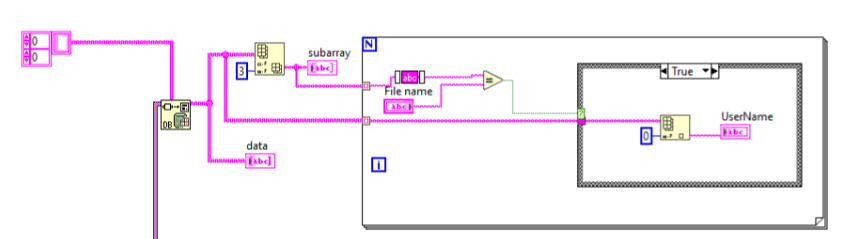
\includegraphics[width=0.6\textwidth]{src/Database/Fragment_DatabaseRead.png}
    \caption{Fragment rozwiązania problemu usuwania białych znaków w SubVi DatabaseRead}
    \label{fig:tab-control-page}
\end{figure}

\subsubsection{\large Problem z ciągłą generacją nowych użytkowników w SubVi DatabaseWrite}

Problem polegał tym, że przy wejściu w zakładkę Add User, program automatycznie uruchamiał SubVi DatabaseWrite i nowy użytkownik był ciągle wpisywany z częstotliwością działania programu nawet jeśli pole do wpisywania
było puste. Zostało to rozwiązane w sposób następujący, do bloku SubVi jako wejście dodano stan kolejki a do samej SubVi strukturę case. W momencie wciśnięcia przycisku Save biometrics
SubVi odpowiedzialne za przechwycenie i zapisanie zdjęcia przesyła również informację o stanie kolejki, jeżeli faktycznie stan zwrócony Face ID: Stop Grab Image się zgadza to program ma wywołać stan 
Add User: Stop Grab Image. Ten stan również jest przesyłany do SubVi, która sprawdza czy taki stan się pojawił i dopiero wtedy jednokrotnie zostanie wywołana co zapobiegło ciągłemu wpisywaniu użytkowników
do bazy i zawieszaniu się programu.

\begin{figure}[H]
    \centering
    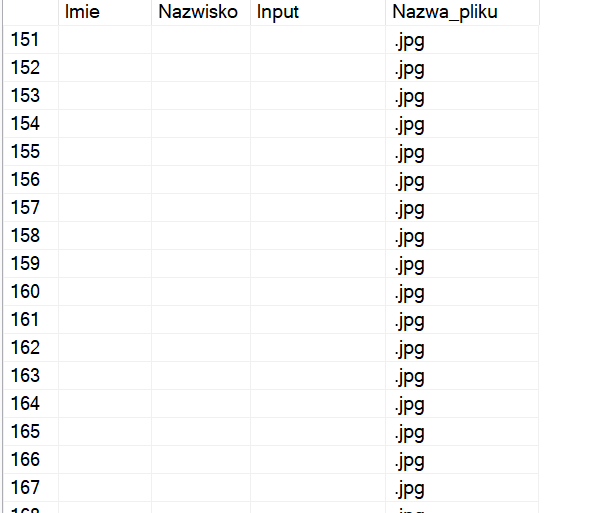
\includegraphics[width=0.4\textwidth]{src/Database/Write_spam.png}
    \caption{Fragment tablicy w bazie danych przedstawiający ciągłe dodawanie nowego użytkownika}
    \label{fig:tab-control-page}
\end{figure}

\begin{figure}[H]
    \centering
    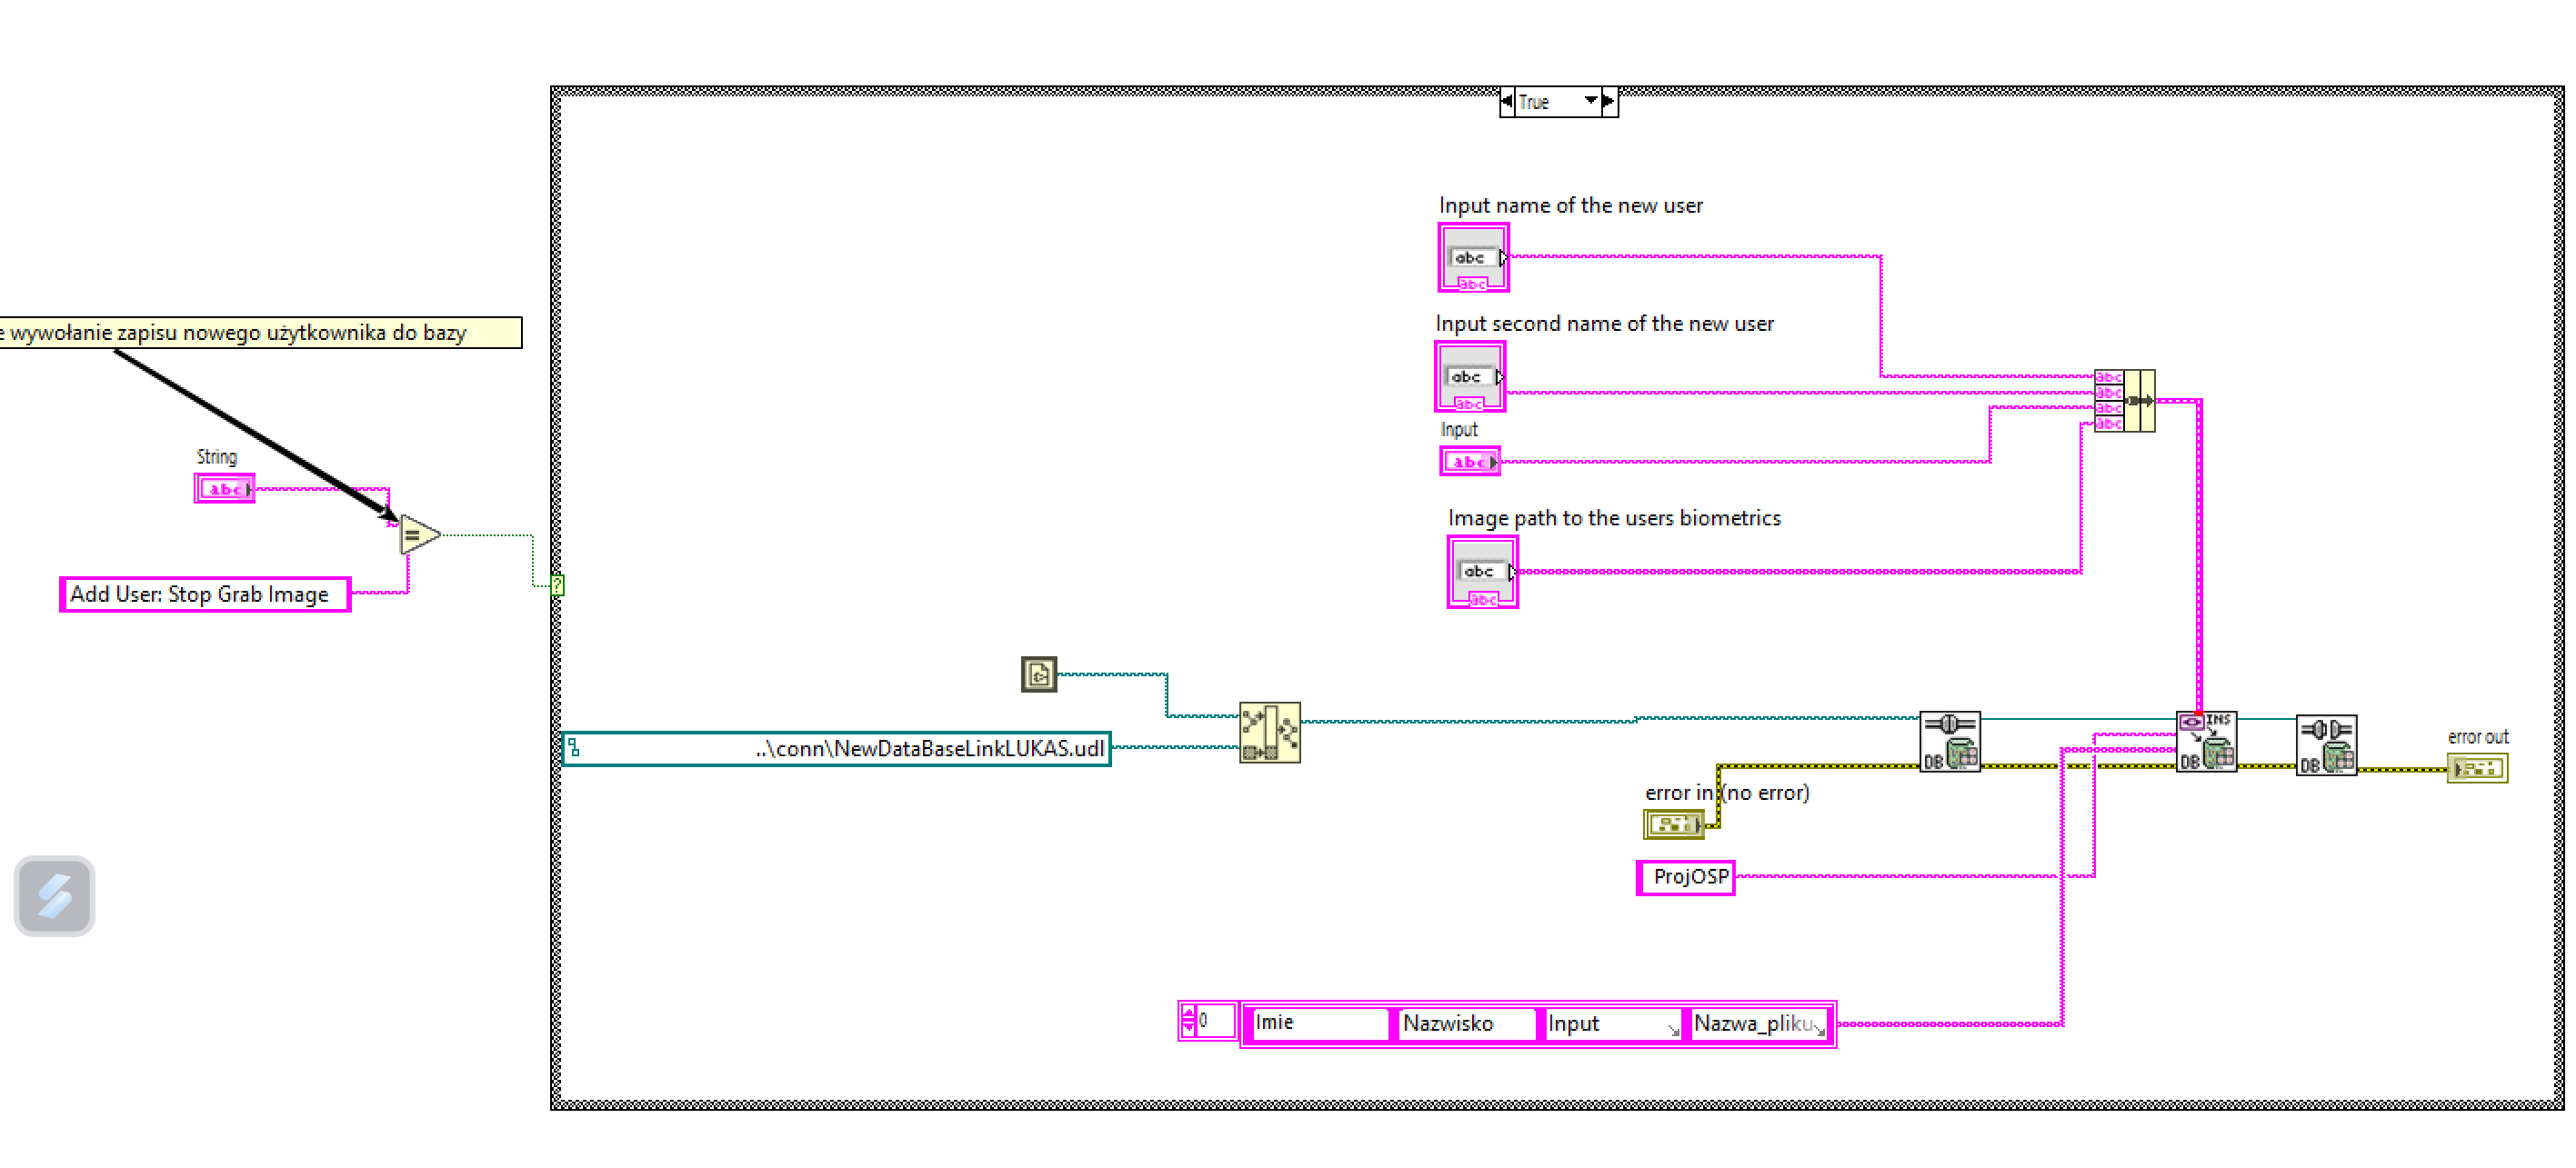
\includegraphics[width=0.9\textwidth]{src/Database/Database_write_subvi.png}
    \caption{Obraz przedstawiający zastosowanie struktury case w SubVi DatabaseWrite}
    \label{fig:first-att}
\end{figure}

\subsubsection{\large Problem logiczny związany z wydobyciem informacji o wierszu w SubVi DatabaseUpdate}

Wykorzystanie gotowego przykładu użycia bloku DB Tools Update Data wiązało się z modyfikacją struktury pod własną tabelę bazy danych.
Konieczne było przesłanie informacji do bloku dla jakiego użytkownika należy zmienić wartości komórki Input. Po analizie programu nasunęły się wnioski
odnośnie, tego iż potrzebny jest indeks wiersza w celu poprawnego zlokalizowania komórki. Aby uzyskać indeks wiersza konieczne było wykorzystanie funkcji for, 
która iterując przez każdy element tabeli porównywała imie wyświetlane po udanym logowaniu z imieniem z bazy. Gdy takie imie zostało odnalezione 
to przesłany zostaje numer iteracji funkcji for dla, której wynik znaleziono. Uzyskany numer iteracji jest jednocześnie numerem indeksu odpowiadający danej osobie.

\begin{figure}[H]
    \centering
    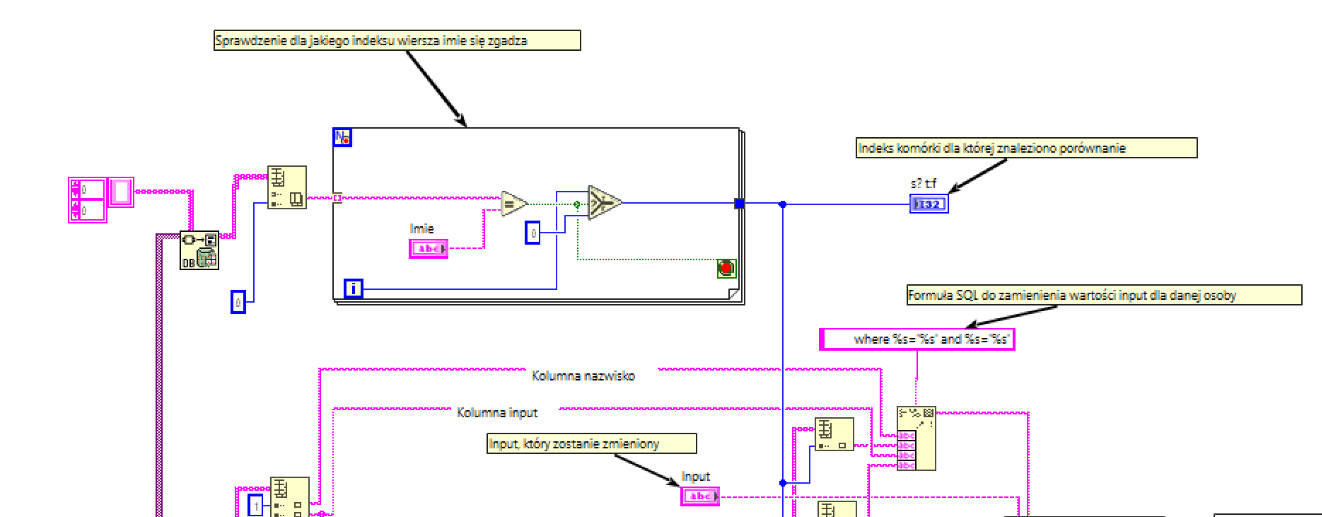
\includegraphics[width=1.0\textwidth]{src/Database/Update_iteration.png}
    \caption{Obraz przedstawiający pozyskiwanie informacji o indeksie osoby w SubVi DatabaseUpdate}
    \label{fig:first-att}
\end{figure}

\section{\LARGE Podsumowanie}

Celem projektu było stworzenie aplikacji do autoryzacji dostępu za pomocą biometrycznej weryfikacji tożsamośći. Główna logika aplikacji została zrealizowana w środowisku LabView, natomiast do rozpoznawania twarzy użyto skryptu napisanego w Pythonie. W ramach projektu zaimplementowano także prostą bazę danych do zarządzania danymi użytkowników. Podczas realizacji projektu napotkano kilka problemów, takich jak trudności z integracją skryptów Python z LabView, problemy z ciągłym dodawaniem nowych użytkowników do bazy danych oraz logiczne błędy związane z wydobywaniem informacji o wierszach w bazie danych. Mimo tych wyzwań, projekt został zakończony sukcesem, spełniając wszystkie założenia i wymagania.

\end{document}
